\documentclass[]{article}

\usepackage{graphicx}

\usepackage{amsmath}

\usepackage{algorithm}

\usepackage[noend]{algpseudocode}

\usepackage[makeroom]{cancel}

\usepackage{lmodern}

\usepackage{empheq}

\newtheorem{theorem}{Teorema}

\usepackage{caption}

\usepackage{mathrsfs}

\newcommand{\highlight}[1]{%
	\colorbox{yellow!20}{$\displaystyle#1$}}

\usepackage[most]{tcolorbox}

\usepackage{pgfplots}
\pgfplotsset{compat = newest}

\newtcbox{\mymath}[1][]{%
	nobeforeafter, math upper, tcbox raise base,
	enhanced, colframe=blue!30!black,
	colback=blue!30, boxrule=1pt,
	#1}

\newtheorem{dimostrazione}{Dimostrazione}

\makeatletter
\def\BState{\State\hskip-\ALG@thistlm}
\makeatother

\usepackage{tikz}
\tikzset{
	treenode/.style = {shape=rectangle, rounded corners,
		draw, align=center},
	root/.style     = {treenode, font=\ttfamily\normalsize},
	env/.style      = {treenode, font=\ttfamily\normalsize},
	dummy/.style    = {circle,draw}
}

\usepackage{multicol}

\setlength{\columnseprule}{0.3pt}
\def\columnseprulecolor{\color{black}}

\newenvironment{Figure}
{\par\medskip\noindent\minipage{\linewidth}}
{\endminipage\par\medskip}

\title{Teoria dell'informazione e crittografia\\ \vspace{3mm} \large{Riassunto videolezioni}}
\author{}
\date{} 

\begin{document}
	

\maketitle

\tableofcontents

\newpage

\section*{Lezione 2}
\addcontentsline{toc}{section}{Lezione 2}


Supponiamo di avere una sorgente S che emette un simbolo ogni colpo di clock.
Questo simbolo subisce una codifica di sorgente (per compattare la rappresentazione dell'informazione) e successivamente, prima di immettere nel canale, bisogna effettuare una codifica di canale.
Il canale è rumoroso per definizione, quindi bisogna aggiungere al simbolo delle cifre di controllo.
Il messaggio quindi sarà composto da \textit{m} bit di messaggio e \textit{k} bit di controllo, il totale farà \textit{n}.

\begin{figure}[h]
	\centering
	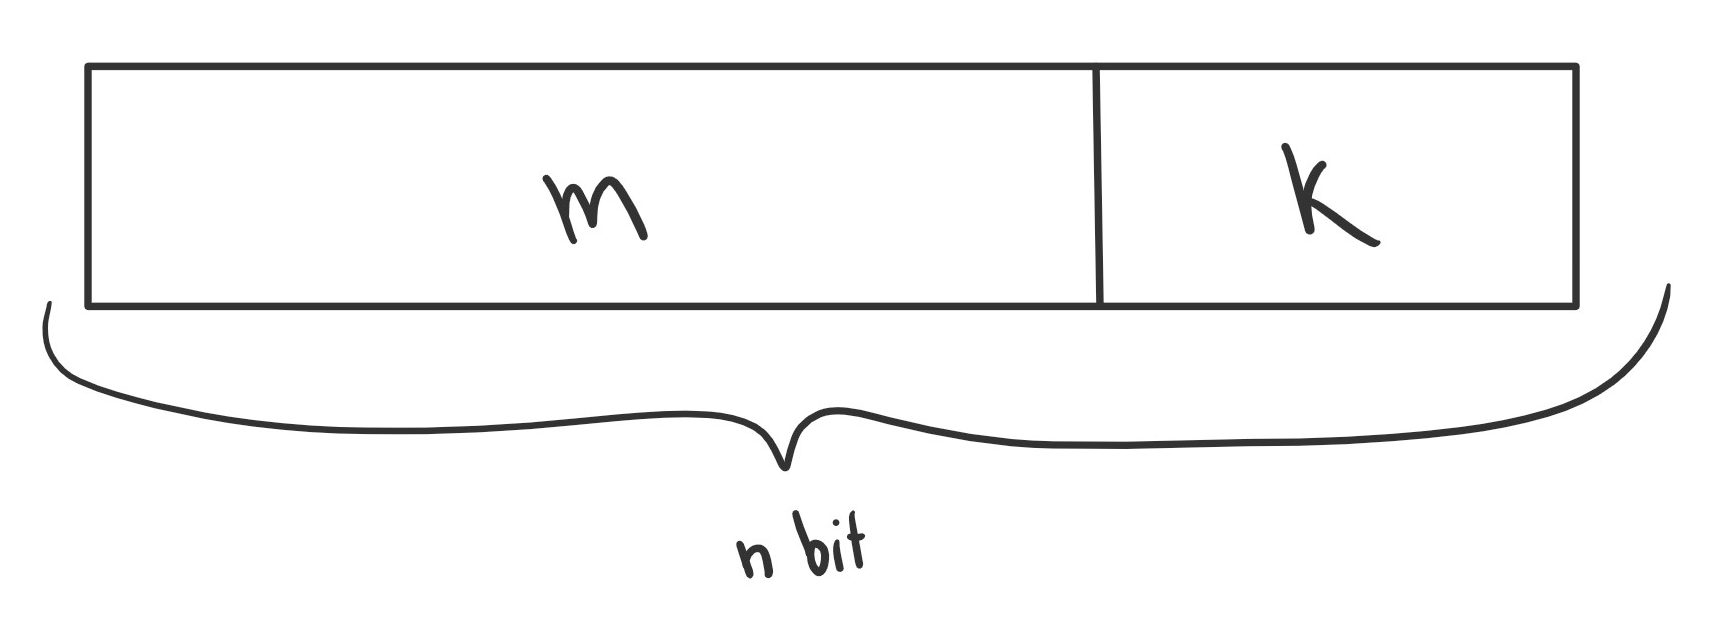
\includegraphics[width=\linewidth]{immagini/img1}
	\caption{Struttura messaggio da inserire nel canale}
\end{figure}

Le cifre di controllo servono ad aumentare la ridondanza del messaggio, in questo modo per il ricevente sarà più facile capire se ci sono stati errori.\\
La \textbf{ridondanza} serve per capire meglio il messaggio (esempio, se togli una lettera dall'alfabeto italiano le parole si capiscono comunque, però con quella lettera è più veloce capire).

\subsection*{Controllo di parità singolo - Codifica di canale}
\addcontentsline{toc}{subsection}{Codifica di canale}

Si aggiunge una cifra alla fine del messaggio.
Ci sono due tipi di parità:
\begin{itemize}
	\item Parità pari: il bit equivale a 1 se il numero di 1 nel messaggio è dispari (in questo modo si arriva ad avere un numero pari di 1).
	il bit equivale a 0 se il numero di 1 nel messaggio è pari (il numero è già pari, quindi non aggiungo altri 1)
	\item Parità dispari: stesso ragionamento ma al contrario.
\end{itemize}

Di base useremo la parità pari, hanno stesse proprietà (in certi casi si usa quella dispari, es. mando pacchetto di zeri su linea con 0 volt).

Per il calcolo del bit di parità si usa una funzione di parità:
\begin{equation}
y = \textrm{Parity(}x_1, x_2, ..., x_n\textrm{)} = x_1 \oplus x_2 \oplus ... \oplus x_n
\end{equation}
In questo modo quando il ricevente legge il messaggio, controlla che il numero di 1 sia pari.
Se non lo è, allora c'è stato un errore singolo.

La stessa funzione può essere vista come:

\begin{equation}
y = \textrm{Parity(}x_1, x_2, ..., x_n\textrm{)} = x_1 + x_2 + ... + x_n \; \text{mod} \; 2
\end{equation}

Questo è utile quando si vuole trattare 0 e 1 con i loro significati numerici.
Isomorfismo fra queste due forme:

\begin{figure}[h]
	\centering
	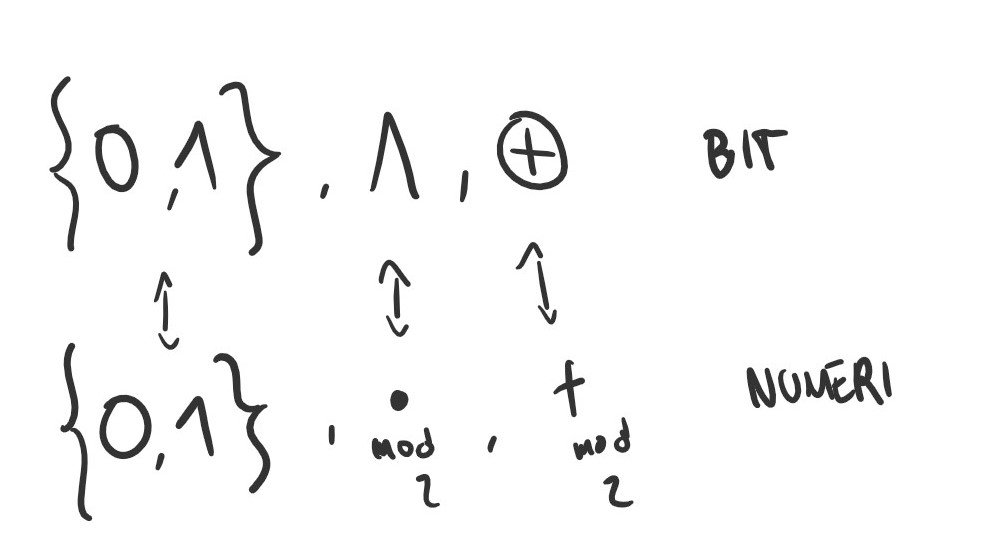
\includegraphics[width=0.6\linewidth]{immagini/img2}
	\caption{Isomorfismo bit/numeri}
\end{figure}

Per fare il calcolo della funzione Parity(\textit{x}) di solito si basa l'hardware (visto che è un operazione molto diffusa, ogni hardware ha supporto per questo tipo di calcoli).
In caso l'hardware supporti solo ad esempio lo xor fra due soli bit, posso scomporre in questo modo ed effettuarne uno ad uno:

\begin{equation}
x_1 \oplus x_2 \oplus x_3 \oplus x_4 \oplus x_5 = (x_1 \oplus x_2) \oplus (x_3\oplus x_4) \oplus (x_5 \oplus 0)
\end{equation}
\begin{center}
n.b.\\
$x \oplus 0 = x$\\
$x \oplus 1 = \lnot x$
\end{center}

Si potrebbe anche utilizzare un automa a stati finiti per modellare il problema:

\begin{figure}[h]
	\centering
	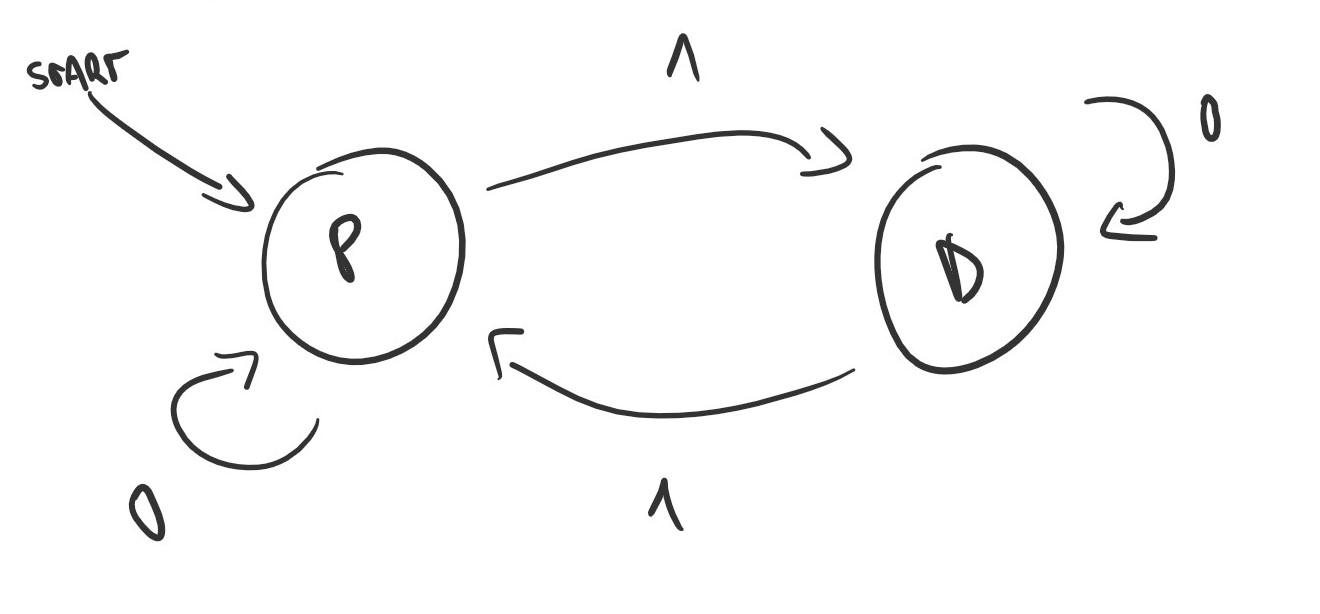
\includegraphics[width=0.6\linewidth]{immagini/img3}
	\caption{Automa a stati finiti per il calcolo pari/dispari}
\end{figure}

\subsection*{Ridondanza}
\addcontentsline{toc}{subsection}{Ridondanza}

Con ridondanza intendiamo, data la Figura 1, questo rapporto:
\begin{equation}
R = \frac{\text{numero di cifre totali}}{\text{numero di cifre di controllo}} = \frac{n}{m} \geq 1
\end{equation}
Con \textit{k = 0} la ridondanza vale 1, e praticamente stiamo inserendo il messaggio senza bit di parità.\\
In altri termini si dice che:
\begin{equation}
R = 1 + \text{eccesso di ridondanza}
\end{equation}
\begin{equation*}
R = 1 + \frac{k}{m}
\end{equation*}
Quando si definisce un metodo per il controllo degli errori, si cerca di avere un eccesso di ridondanza minore possibile (meno bit si usano nel canale, meno errori avverranno; ma in generale meglio ottimizzare).

Quanto vale la ridondanza nel caso del controlli di parità?

\begin{equation}
R_{\text{parity}} = \frac{n}{n-1} = \frac{(n-1)+1}{n-1} = 1 + \frac{1}{n-1}
\end{equation}

Quindi l'eccesso di ridondanza è $\frac{1}{n-1}$.

Ovviamente, osservando come l'eccesso di ridondanza sia uguale a $\frac{k}{m}$, a parità di \textit{m}, il numero di bit del messaggio, il modo di ridurre al minimo la ridondanza è quello di minimizzare il numeratore, quindi la \textit{k}.
In gergo si dice che ogni cifra di controllo dovrà \textit{coprire} il maggior numero di bit di messaggio possibile, per avere una bassa ridondanza.


\subsection*{Canale - modelli di rumore}
\addcontentsline{toc}{subsection}{Canali - Modelli di rumore}

Il canale più semplice e facile da gestire è il \textbf{rumore bianco}, definito da queste proprietà:
\begin{itemize}
	\item La probabilità che avvenga un errore in ciascuna posizione è uguale a \textit{p} per ogni bit.
	Di conseguenza la probabilità che la trasmissione avvenga in modo corretto è $1-p$.
	\item Il fatto che avvenga un errore in posizione \textit{i} non influisce sulle altre probabilità, quindi si parla di eventi statisticamente indipendenti (condizione che rende poco realistico il rumore bianco, es. sbalzo di corrente).
\end{itemize}

Nell'intero pacchetto, qual è la probabilita di avere \textit{k} errori, dato $0 \leq k \leq n$?
Ragioniamo prima sul valore di \textit{p}
\begin{itemize}
	\item $p = 0$? No, impossibile che in un canale ci sia completa assenza di errore (qualunque supporto io utilizzi, col tempo si deteriora).
	\item $p = 1$? No, se no basta una porta not al ricevitore per avere tutti i bit corretti (come prima).
	\item $p > \frac{1}{2}$? Potrebbe aver senso, però se ho un canale che sbaglia più della metà delle volte, basta una porta not per ridurre questa quantità fino a una quantità minore di $\frac{1}{2}$ 
	\item $p = \frac{1}{2}$? Così ottengo un generatore di numeri casuali perfetto in quanto ogni bit viene trasformato in modo casuale in 0 o in 1 (cosa impossibile).
\end{itemize}

Possiamo concludere dicendo che \textit{p} è sempre $0 < p < \frac{1}{2}$.

Tornando alla domanda di prima, quanto è la probabilità di avere \textit{k} errori?\\
Partiamo dalla probabilità di avere 1 errore, esso può avvenire in una posizione qualsiasi.
Essendo eventi stocastici e statisticamente indipendenti, la probabilità di un errore è uguale a
\begin{equation}
p(\text{1 errore}) = p(E_1 \lor E_2 \lor ... \lor E_n)
\end{equation}
Con $E_k$ s'intende l'evento che avvenga un errore in posizione \textit{k}.\\
Quanto è la probabilità che avvenga un errore \textit{solo} nella posizione 2?
\begin{equation}
p(\text{errore in pos 2}) = (1-p) \; p \; (1-p)(1-p) \; ... \; (1-p)
\end{equation}
\begin{equation*}
= p \; (1-p)(1-p) \; ... \; (1-p)
\end{equation*}
\begin{equation*}
= p \; (1-p)^{n-1}
\end{equation*}

Ovviamente al posto della seconda posizione, questa regola vale per ogni posizione (proprietà commutativa della moltiplicazione).

Quindi la probabilità di avere un solo errore:
\begin{equation}
p(\text{1 errore}) = p(\text{errore in pos 1}) + p(\text{errore in pos 2}) + \; ... \; + p(\text{errore in pos n})
\end{equation}
\begin{equation*}
= np(1-p)^{n-1}
\end{equation*}

E la probabilità di ottenere 2 errori?\\
Vediamo prima la probabilità di ottenere 2 errori in 2 posizioni fissate:
\begin{equation}
p(\text{errori in pos 1 e 2}) = p \cdot p \; (1-p)(1-p) \; ... \; (1-p)
\end{equation}
\begin{equation*}
= p^2 \; (1-p)(1-p) \; ... \; (1-p)
\end{equation*}
\begin{equation*}
= p^2 \; (1-p)^{n-2}
\end{equation*}

Come posso creare le combinazioni di queste posizioni?

\begin{equation}
\binom{n}{2} = \frac{n(n-1)}{2}
\end{equation}

Quindi questo è il numero di modi in cui posso disporre gli errori nel pacchetto

Da qui, la probabilità di ottenere 2 errori è:

\begin{equation}
p(\text{2 errori}) = \binom{n}{2} p^2 (1-p)^{n-2}
\end{equation}

Riprendendo la probabilità di avere un errore, essa si può riscrivere come:

\begin{equation}
p(\text{1 errore}) = \binom{n}{1} p^1 (1-p)^{n-1}
\end{equation}

Ora, generalizzando, si può rispondere alla domanda: qual è la probabilità che si verifichino \textit{k} errori in un messaggio di \textit{n} bit (errori disposti in qualsiasi posizione all'interno del pacchetto)?

\begin{equation}
p(\text{k errori}) = \binom{n}{k} p^k (1-p)^{n-k} \; \; \; \; \; \; \text{per} \; 0 \geq k \geq n
\end{equation}

Vediamo ora come si comporta la funzione $p(\text{errori})$ dati un \textit{n} e un \textit{p} fissati.
\begin{figure}[h]
	\centering
	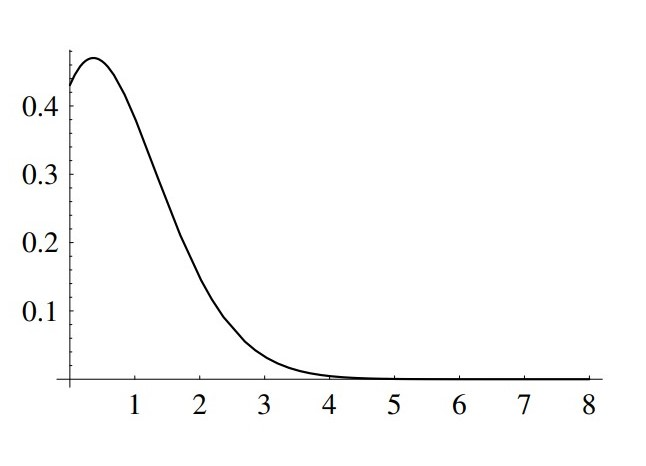
\includegraphics[width=0.6\linewidth]{immagini/img4}
	\caption{Grafico di $\binom{n}{k}p^k (1-p)^{n-k}$ con $n=8$ e $p=0.1$}
\end{figure}

Ma se all'interno del pacchetto avviene un numero pari di errori? Il controllo di parità fallisce in quanto il numero di 1 è pari (numero pari di 1 iniziale + numero pari di errori = numero pari di 1).
Viceversa se il numero di errori è dispari, allora il controllo di parità se ne accorge.

Quanto è la probabilità che il controllo di parità fallisca? In altri termini: quanto è la probabilità che avvenga un numero pari di errori?

Procediamo per passi; recuperiamo la probabilità di commettere un errore dall'equazione (13):

\begin{equation}
p(\text{1 errore}) = \binom{n}{1} p^1 (1-p)^{n-1}
\end{equation}
\begin{equation*}
= np(1-p)^{n-1}
\end{equation*}

Ricordiamo un'approssimazione sfruttando le serie di Taylor:

\begin{equation}
(1+x)^{\alpha} \approx 1 + \alpha x \; \; \; \; \; \; \text{per} \; |x| < 1
\end{equation}

Possiamo considerare \textit{n} come molto minore di $\frac{1}{p}$, quindi scrivere:

\begin{equation}
np(1-p)^{n-1}
\end{equation}
\begin{equation*}
\approx np[1-p(n-1)] 
\end{equation*}
\begin{equation*}
= np[1-p(n-1)]
\end{equation*}
\begin{equation*}
= np[1-np+p]
\end{equation*}
\begin{equation*}
= np[1-np+p]
\end{equation*}
\begin{equation*}
np-n^2p^2+np^2 
\end{equation*}

Ora trascuriamo i termini con $p^2$ in quanto essendo minore di 1, dominerà \textit{p}; quindi

\begin{equation}
p(\text{1 errore})\approx np
\end{equation}
\begin{equation*}
= \binom{n}{1}p
\end{equation*}

Per due errori:

\begin{equation}
p(\text{2 errori})\approx np \binom{n}{2}p^2
\end{equation}
\begin{equation*}
= \binom{n}{2}p^2
\end{equation*}

Generalizzando per \textit{k} errori:

\begin{equation}
p(\text{\textit{k} errori})\approx np \binom{n}{k}p^k
\end{equation}

Quindi, tornando al problema di prima, dobbiamo fare un'osservazione:

\begin{equation}
	\sum_{k=0}^{n} \binom{n}{k} p^k(1-p)^{n-k} = 1
\end{equation}

Se sommo tutte le probabilità, fare zero errori, fare un errore, fare due errori ecc. ovviamente ho come somma 1 (evento stocastico).

Sfrutto questa proprietà:
\begin{equation}
(a+b)^n = \sum_{k=0}^{n} \binom{n}{k} a^kb^{n-k}
\end{equation}

\bigskip
\bigskip

... 
Lezione 02 parte 3 min 33 +-
...

\bigskip
\bigskip
Quindi la probabilità che il controllo di parità fallisca è
\begin{equation}
p(\text{controllo parità fallisce}) = \frac{1 + (1-2p)^n}{2}-(1-p)^n
\end{equation}

\subsection*{Burst di errori}
\addcontentsline{toc}{subsection}{Burst di errori}

Gli errori nella realtà avvengono in maniera non indipendente, di solito avvengono errori su sequenze di bit adiacenti.
Definiamo \textit{L} come lunghezza del \textbf{burst} di errori.

La parola \texttt{ciao} in ASCII è rappresentata in questo modo:
\begin{center}
	\texttt{C} = 1000011\\
	\texttt{I} = 1001001\\
	\texttt{A} = 1000001\\
	\texttt{O} = 1001111
\end{center}

... fine lezione 02 parte 3









\newpage
\section*{Lezione 3}
\addcontentsline{toc}{section}{Lezione 3}

\subsection*{Codici pesati}
\addcontentsline{toc}{subsection}{Codici pesati}
Dato un messaggio da spedire nel canale, si associa ad esso un insieme di valori.
Ad esempio, dato un messaggio $m = m_1 \; m_2 \; ... \; m_n$, codifichiamo ogni $m_i$ nel seguente modo:
\begin{center}
	26 lettere A-Z\\
	1 spazio \textvisiblespace\\
	10 cifre 0-9\\
	$\downarrow$\\
	37 simboli
\end{center}

Successivamente si associa ad ogni messaggio un insieme di valori di \textit{peso}:

\begin{center}
	 msg: $m_1, \; m_2, \; ... \; m_n, \; c$\\
	 pes: $n+1, \; n, ... \; 2, \; 1 $
\end{center}

Facciamo un esempio, mettiamo di voler spedire la parola \texttt{ciao}, utilizzando la codifica mostrata in precedenza.

\begin{table}[h]
	\centering
	\begin{tabular}{llllll}
		& \texttt{C} & \texttt{I} & \texttt{A} & \texttt{O}  & check \\
		\hline
		msg & 2 & 8 & 0 & 14 & check \\
		pes & 5 & 4 & 3 & 2  & 1    
	\end{tabular}
\end{table}

Il mittente pesa ogni carattere molitplicando la codifica per il peso:

\begin{equation*}
	2 \cdot 5 + 8 \cdot 4 + 0 \cdot 3 + 14 \cdot 2 + check \cdot 1
\end{equation*}

Succcessivamente si pone questa espressione uguale a 0 \textit{mod} 37 (questo è il numero totale di caratteri).

\begin{equation*}
2 \cdot 5 + 8 \cdot 4 + 0 \cdot 3 + 14 \cdot 2 + check \cdot 1 = 0 \; mod \; 37
\end{equation*}
\begin{equation*}
70 + check = 0 \; mod \; 36
\end{equation*}
\begin{equation*}
check = 4
\end{equation*}

Successivamente spedisce il messaggio con il vettore dei pesi.\\
Il ricevitore si calcola il peso (usando il valore di \textit{check} spedito dal mittente) e controlla che il peso sia uguale a 0 \textit{mod} 37.

Da notare che 37 è primo, quindi ci va bene perchè lavoriamo in un campo.\\
Ad esempio i conti in modulo 6 hanno i divisori di zero (3 $\cdot$ 2 = 0 mod 6).
Se non è primo piuttosto aumentiamo il numero di caratteri (piuttosto non li usiamo, ma ci semplifica tutto avere un numero primo).

I codici pesati sono utili per individuare errori come ad esempio lo scambio di caratteri, l'inserimento di caratteri da parte del canale ecc...

\medskip

Ad esempio, se all'interno di un messaggio al posto di \texttt{ab} viene inviato \texttt{ba}, allora la differenza fra le somme pesate è (fissato \textit{k+1} come peso di \texttt{a}, \textit{k} come peso di \texttt{b}).

\begin{equation*}
a(k+1)+bk \rightarrow b(k+1)+ak
\end{equation*}
\begin{equation*}
a(k+1)+bk - b(k+1)+ak = 
\end{equation*}
\begin{equation*}
= b(k+1)+ak - a(k+1) -bk
\end{equation*}
\begin{equation*}
= bk +b+ak-ak-a-bk
\end{equation*}
\begin{equation*}
= b-a
\end{equation*}

Quindi il messaggio viene accettato solo se la differenza è uguale a 0, quindi quando $b-a = 0 \; mod \; 37$, ma per essere 0 allora i due caratteri devono essere uguali.
Se due simboli uguali vengono scambiati quindi, il messaggio viene accettato lo stesso.

Vediamo un algoritmo per calcolare i pesi:

\begin{algorithm}
	\begin{algorithmic}[1]
		\Procedure{CalcolaCheckDigit}{}
		\State $\textit{sum} \gets 0$
		\State $\textit{ssum} \gets 0$
		\While{\textit{not} EOF}
		\State read $\textit{symbol}$
		\State $sum \gets sum + \textit{symbol} \; \text{mod} \; 37$
		\State $ssum \gets ssum + \textit{sum} \; \text{mod} \; 37$
		\EndWhile
		\State $temp \gets ssum + sum \; \text{mod} \; 37$
		\State $c \gets 37 - temp \; \text{mod} \; 37$
		\State return $c$
		\EndProcedure
	\end{algorithmic}
\end{algorithm}

Una simulazione dell algoritmo con la parola \texttt{ciao} è la seguente:

\begin{table}[h]
	\centering
	\begin{tabular}{l|l|l}
		msg & sum & ssum   \\
		\hline
		\texttt{C} = 2  & 2   & 2      \\
		\texttt{I} = 8  & 10  & 12     \\
		\texttt{A} = 0  & 10  & 22     \\
		\texttt{O} = 14 & 24  & 46 $\equiv$ 9
	\end{tabular}
\end{table}
\vspace{-5mm}
\begin{equation*}
temp \leftarrow 9 + 24 \equiv 33\\
\end{equation*}
\begin{equation*}
c \gets 37 - 33 = 4 \equiv \texttt{E}
\end{equation*}

\medskip

Quindi il messaggio spedito sarà \texttt{ciaoe}.

\newpage

Il ricevente ricalcolerà la tabella usando il messaggio appena arrivato:

\begin{table}[H]
	\centering
	\begin{tabular}{l|l|l}
		msg & sum & ssum   \\
		\hline
		\texttt{C} = 2   & 2   & 2      \\
		\texttt{I} = 8   & 10  & 12     \\
		\texttt{A} = 0   & 10  & 22     \\
		\texttt{O} = 14   & 24  & 46 $\equiv$ 9 \\
		\texttt{E} = 4  & 28  & 37 $\equiv$ \textbf{0}
	\end{tabular}
\end{table}

La somma delle somme finale è 0, quindi il messaggio è ok. Se non fosse 0, allora il messaggio è stato modificato, ma non posso sapere dove.

Astraiamo il procedimento appena utilizzato:

\begin{table}[H]
	\centering
	\begin{tabular}{l|l|l}
		msg & sum & ssum   \\
		\hline
		\texttt{w}  & $w$   & 2      \\
		\texttt{x}  & $w+x$  & $2w+$x     \\
		\texttt{y}  & $w+x+y$ & $3w+2x+y$    \\
		\texttt{z}  & $w+x+y+z$  & $4w+3x+2y+z$ \\
		\texttt{c}  & $w+x+y+z+c$  & $5w+4x+3y+2z+c \equiv 0 \; mod \; 37$ 
	\end{tabular}
\end{table}

Si noti come la somma delle somme assegna un peso decrescente a tutti i caratteri: 5 a \textit{w}, 4 a \textit{x} e così via...

Il codice ISBN è un esempio di codice pesato su base 11; proviamo a verificare il seguente codice: 1-58488-508-4

\begin{table}[H]
	\centering
	\begin{tabular}{l|l|l}
		msg & sum & ssum   \\
		\hline
		\texttt{1}  & 1   & 1      \\
		\texttt{5}  & 6  & 7     \\
		\texttt{8}  & $14 \equiv 3$ & 10   \\
		\texttt{4}  & $7$  & $17 \equiv 6$ \\
		\texttt{8}  & $15 \equiv 4$  & 10 \\
		\texttt{8}  & $12 \equiv 1$  & $11 \equiv 0$ \\
		\texttt{5}  & $6$  & 6 \\
		\texttt{0}  & $6$  & $12 \equiv 1$ \\
		\texttt{8}  & $14 \equiv 3$  & 4 \\
		\hline
		\texttt{4}  & $7$  & $11 \; mod \; 11 \equiv \textbf{0}$ \\
	\end{tabular}
\end{table}

Quindi il codice è corretto. Nel caso l'ultima cifra fosse un 10 si inserisce una \texttt{x}.

\newpage 
\subsection*{Es. 2.4 - 1, pag.24}
Caso: rumore bianco\\
$p=0.001$ (probabilità errore in ogni posizione)\\
$n=100$ (dimensione pacchetto)\\

Quanto è la probabilità che ci siano 0 errori?

\begin{equation*}
p(\text{0 errori}) = (1-p)^n
\end{equation*}
\begin{equation*}
= (1-\frac{1}{1000})^{100}
\end{equation*}
\begin{equation*}
= e^{100 \cdot ln(1 - \frac{1}{1000})}
\end{equation*}
\begin{equation*}
\approx e^{100 \cdot ln(-\frac{1}{1000})}
\end{equation*}
\begin{equation*}
= e^{-\frac{1}{10}}
\end{equation*}

\subsection*{Es. 2.4 - 2, pag.25}
Caso: rumore bianco\\
$p=0.001$ (probabilità errore in ogni posizione)\\
$n=100$ (dimensione pacchetto)\\

Quanto è la probabilità di non riuscire ad individuare un errore?

Per rispondere a questa domanda, possiamo rispondere a: quanto è la probabilità che il controllo di errore singolo sbagli?

Ricordando l'equazione (23):

\begin{equation*}
p(\text{controllo parità fallisce}) = \frac{1 + (1-2p)^n}{2}-(1-p)^n
\end{equation*}
\begin{equation*}
= \frac{1 + (1-\frac{2}{1000})^{100}}{2}-(1-\frac{1}{1000})^{100}
\end{equation*}
\begin{equation*}
\approx 0.0045
\end{equation*}

\subsection*{Codici a correzione d'errore}
I codici a correzione d'errore, a differenza del controllo di parità, permette al ricevente di rilevare dove è avvenuto un errore ed eventualmente di correggerlo.
Questo ovviamente richiede di aggiungere delle cifre di controllo ulteriori.

\newpage
\subsubsection*{Codici rettangolari - 1 Errore}
Il messaggio inserito nel canale viene rappresentato come un rettangolo (logicamente parlando, non fisicamente).
Rappresentiamo i bit di messaggio in questo modo:
\medskip
\begin{equation*}
\begin{matrix}
\textit{o} & \textit{o} & \textit{o} & ... & \textit{o} & x\\
\textit{o} & \textit{o} & \textit{o} & ... & \textit{o} & x\\
\vdots & \vdots & \vdots & \ddots & \vdots & \vdots\\
\textit{o} & \textit{o} & \textit{o} & ... & \textit{o} & x\\
x & x & x & ... & x & 
\end{matrix}
\end{equation*}
Nell'esempio il carattere \textit{o} rappresenta un bit di messaggio, \textit{x} rappresenta un carattere di controllo.
Ogni cifra di controllo sulle righe codifica la riga corrispondente, quelle sulle colonne codificano la colonna.

In questo modo, se un bit di messaggio viene modificato, posso individuare subito l'errore in quanto verranno sbagliati i bit di controllo sulla relativa riga e colonna.
Ad esempio, se un bit in posizione $i, j$ viene alterato, allora i due controlli di parità sulla riga $i$ e sulla colonna $j$ falliranno, ma il ricevente intuisce subito quale bit ha subito modifiche.\\

Per capire quanto il metodo è efficiente, andiamo a calcolarne la ridondanza:

\begin{equation}
R = \frac{m \cdot n}{(m-1)(n-1)}
\end{equation}
\begin{equation*}
= 1 + \frac{1}{m-1} + \frac{1}{n-1} + \frac{1}{(m-1)(n-1)}
\end{equation*}

Quindi l'eccesso di ridondanza equivale a $\frac{1}{m-1} + \frac{1}{n-1} + \frac{1}{(m-1)(n-1)}$.\\
Quanto è l'eccesso di ridondanza più piccola possibile in questa classe di codici (codici rettangolari)?
L'idea è quella di minimizzare la funzione
\begin{equation*}
\frac{1}{m-1} + \frac{1}{n-1} + \frac{1}{(m-1)(n-1)}
\end{equation*}
Si dovrebbero quindi calcolare le derivate parziali rispetto a \textit{n} e a \textit{m} e vedere quando si annullano, ma è facilmente intuibile che questa quantità è la minore possibile quando $m=n$.

Per cui i più efficienti sono i codici \textbf{quadrati}, ovvero il sottoinsieme di codici rettangolari in cui il numero di righe è uguale al numero di colonne.

La loro ridondanza vale
\begin{equation*}
R = \frac{n^2}{(n-1)^2} = 1 + \frac{2}{n-1} + \frac{1}{(n-1)^2}
\end{equation*}

I peggiori invece, sono i codici con una singola riga (i bit di controllo sono di più dei bit di messaggio!)














\newpage
\section*{Lezione 4}
\addcontentsline{toc}{section}{Lezione 4}

Seguendo l'esempio dei codici rettangolari, proviamo a disporre ora i bit di messaggio in altre forme logiche, in modo da coprire il più gran numero di bit di messaggio con ogni bit di controllo.

\subsection*{Codici triangolari - 1 Errore}
\addcontentsline{toc}{subsection}{Codici triangolari}
Proviamo a creare una forma logica di un codice triangolare:

\begin{equation*}
\begin{matrix}
\textit{o} & \textit{o} & \textit{o} & \textit{o} & x\\
\textit{o} & \textit{o} & \textit{o} & x\\
\textit{o} & \textit{o} & x\\
\textit{o} & x\\
x
\end{matrix}
\end{equation*}

Ovviamente il numero di bit di messaggio deve consentire una costruzione di questo genere (dagli antichi greci: numeri triangolari).

Come prima, ogni bit di controllo copre la relativa colonna e riga.

Quanto vale la ridondanza di questo tipo di codici?

Il numero di bit totali è 
\begin{equation}
\sum_{i=1}^{n}i = \frac{n(n+1)}{2}
\end{equation}
mentre il numero di bit di messaggio è
\begin{equation}
\sum_{i=1}^{n-1}i = \frac{(n-1)(n-1+1)}{2} = \frac{(n-1)n}{2}
\end{equation}

Per cui passiamo a calcolare la ridondanza:

\begin{equation}
R_{triangolare} = \frac{\frac{n(n+1)}{2}}{\frac{(n-1)n}{2}}
\end{equation}
\begin{equation*}
= \frac{\cancel{n}(n+1)}{\cancel{2}} \cdot \frac{\cancel{2}}{(n-1)\cancel{n}}
\end{equation*}
\begin{equation*}
= \frac{(n+1)}{(n-1)}
\end{equation*}
\begin{equation*}
= \frac{(n-1) + 2}{(n-1)}
\end{equation*}
\begin{equation*}
= 1 + \frac{2}{(n-1)}
\end{equation*}

\newpage

Da qui, l'eccesso di ridondanza vale

\begin{equation}
\frac{2}{(n-1)}
\end{equation}

Confrontiamolo con l'eccesso di ridondanza dei codici quadrati:

\begin{equation*}
ecc_{quadrato} = \frac{2}{n-1}+\frac{1}{(n-1)^2}
\end{equation*}
\begin{equation*}
ecc_{triangolo} = \frac{2}{n-1}
\end{equation*}

Si nota ovviamente come i codici triangolari siano sicuramente più efficienti.

\subsection*{Codici cubici - 1 Errore}
\addcontentsline{toc}{subsection}{Codici cubici}

Un'altra disposizione che si può seguire per ordinare i bit di messaggio è a forma cubica.

\begin{figure}[h]
	\centering
	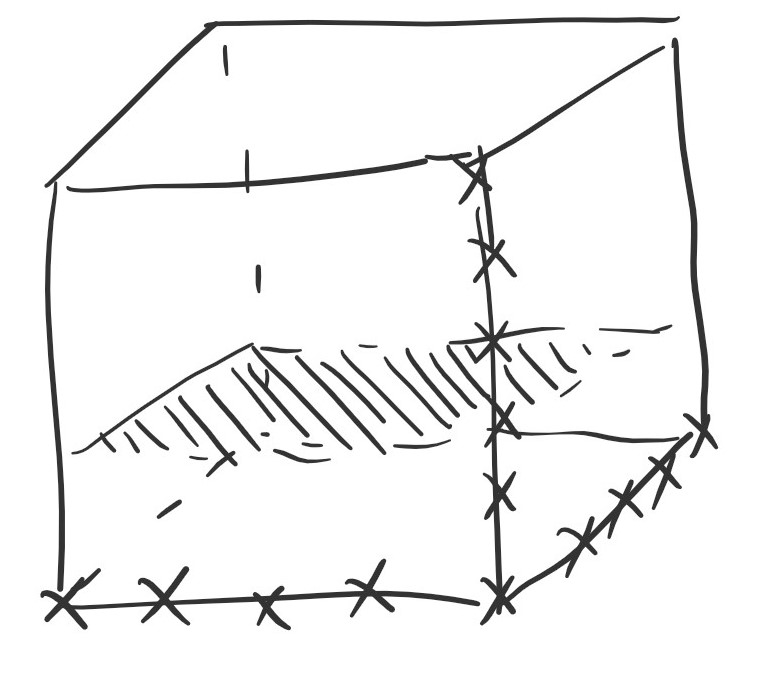
\includegraphics[width=0.6\linewidth]{immagini/img5}
\end{figure}

Facendo dei conti \textit{a spanne}, ci sono $n^3$ posizioni, le cifre di controllo sono $3(n-1) + 1 = 3n-2$.

La ridondanza più o meno quindi vale

\begin{equation}
R = \frac{(n-1)^3+3n-2}{(n-1)^3} \approx 1 + \frac{3}{n^2}
\end{equation}

Seguendo questo ragionamento, potrei pensare di aumentare le dimensioni

\subsection*{Codici ipercubici}
\addcontentsline{toc}{subsection}{Codici ipercubici}

Seguendo il modello dei \textit{conti a spanne}, diciamo più o meno che le cifre di messaggi è $(n-1)^4$, mentre le check digit saranno $4(n-1)+1=4n-3$.

La ridondanza quindi varrà:

\begin{equation}
R = 1 + \frac{4n-3}{(n-1)^4} \approx 1 + \frac{4}{n^3}
\end{equation}

Da qui si nota come si può passare a ragionare in \textit{k} dimensioni, e si possono tirare delle conclusioni:

\begin{equation}
(n-1)^k \; \; \; \text{bit di messaggio}
\end{equation}
\begin{equation*}
k(n-1)+1 = kn-k+1 \; \; \; \text{bit di controllo}
\end{equation*}
\begin{equation*}
R = 1 + \frac{kn-k+1}{(n-1)^k} \approx 1 + \frac{k}{n^{k-1}} \; \; \; \text{ridondanza}
\end{equation*}

\smallskip

Da qui si nota come la ridondanza decresce in maniera polinomiale, possiamo fare di meglio?

\subsection*{Codici di Hamming}
\addcontentsline{toc}{subsection}{Codici di Hamming}

Codici ottimali per individuare e correggere 1 errore (al massimo) in un canale caratterizzato da rumore bianco.
Cosa significa codici ottimali? Il rapporto fra cifre di controllo e cifre di messaggio è esponenziale, meglio di così non si può fare.

Da ora in poi ci riferiremo con \textit{k} alle cifre di messaggio, \textit{m} alle cifre di controllo. \textit{n} sarà la loro somma.

Le combinazioni (configurazioni) di cifre di controllo sono $2^m$.
Da notare come deve sempre valere $2^m \geq n+1$, questo è necessario in quanto ci dev'essere una configurazione per ogni posizione di errore, più uno (configurazione per rappresentare zero errori).
Altrimenti non abbiamo abbastanza configurazioni per rappresentare tutte le situazioni (errore in posizione 3, errore in posizione 8, ecc).\\

Supponiamo di voler mandare un messaggio di 7 bit, ci chiediamo quanti di questi bit possono essere di messaggio e quanti di controllo?

\begin{equation*}
2^m \geq 8 \rightarrow m \geq 3 \rightarrow m=3
\end{equation*}
\begin{equation*}
k = 7 - 3 = 4
\end{equation*}

\newpage

Oppure posso chiedermi: devo inviare 4 cifre di messaggiosul canale, di quante cifre di controllo ho bisogno?

\begin{equation*}
2^m \geq n+1 \rightarrow 2^m \geq m+k+1 \rightarrow 2^m \geq m+5
\end{equation*}

Quando è vero $2^m \geq m+5$? Proviamo ad assegnare dei valori a \textit{m}:

\begin{table}[h]
	\centering
	\begin{tabular}{l|l|l}
		$m$ & $2^m$ & $m+5$ \\
		\hline
		1   & 2     & 6     \\
		2   & 4     & 7     \\
		3   & 8     & 8     \\
		4   & 16    & 9    
	\end{tabular}
\end{table}

Il valore più piccolo che ci va bene è proprio 3, quindi l'ideale è utiliazzare 3 cifre di controllo.

Ciascuna cifra di controllo fa il controllo di parità su diverse cifre di messaggio. Facciamo un esempio:\\
Ho 9 cifre di messaggio, avrò quindi 3 cifre di controllo, come si suddividono le cifre per il calcolo delle parità?


\begin{equation}
c_1 = x_1 \oplus x_2 \oplus x_5 \oplus x_7
\end{equation}
\begin{equation*}
c_2 = x_5 \oplus x_7 \oplus x_8 \oplus x_9
\end{equation*}
\begin{equation*}
c_3 = x_1 \oplus x_2 \oplus x_8 \oplus x_9
\end{equation*}

Ma quanto vale la somma di $c_1$ e $c_2$ (ricordando che $x \oplus 0 = x$)?

\begin{equation*}
c_1 \oplus c_2 = x_1 \oplus x_2 \oplus x_8 \oplus x_9
\end{equation*}

che è esattamente uguale a $c_3$!

Allo stesso modo considerando vettori binari di \textit{n} elementi, una somma in modulo due e un prodotto modulo due, posso effettuare il calcolo in questo modo:

\begin{equation}
v_1 = (1,1,0,0,1,0,1,0,0)
\end{equation}
\begin{equation*}
v_2 = (0,0,0,0,1,0,1,1,1)
\end{equation*}
\begin{equation*}
\downarrow
\end{equation*}
\begin{equation*}
v_1 + v_2 = (1,1,0,0,0,0,0,1,1) \; \; \; \; \; \; \; \, \,
\end{equation*}


Questo insieme, composto da ($\{0,1\}^n, +_2, \cdot$) è uno spazio vettoriale, quindi le tre equazioni di parità considerate sono linearmente dipendenti, e questo ovviamente è da evitare visto che la terza equazione non da informazione in quanto è ricavabile dalle altre due.

\newpage 

Ripendendo l'esempio del pacchetto di 7 bit, scriviamo questa tabella che rappresenta le posizioni:

\begin{table}[h]
	\centering
	\begin{tabular}{l|l}
		pos & pos in binario \\
		\hline
		1   & 001            \\
		2   & 010            \\
		3   & 011            \\
		4   & 100            \\
		5   & 101            \\
		6   & 110            \\
		7   & 111        \\
		0 (nessun errore) & 000    
	\end{tabular}
\end{table}

Da notare come i bit necessari per coprire tutte le posizioni sono 3, esattamente come il numero di bit di controllo.
L'insieme delle posizioni in valore binario assume il nome di \textit{sindrome}.
Se la sindrome vale 101 allora è avvenuto un errore in posizione 5.
Non ci resta che capire come assegnare le posizioni per ogni bit.

Definiamo le cifre di controllo come le colonne della tabella precedente, quindi:

\begin{table}[h]
	\centering
	\begin{tabular}{l|lll}
		\hline
		1   & 0 & 0 & 1            \\
		2   & 0 & 1 & 0            \\
		3   & 0 & 1 & 1            \\
		4   & 1 & 0 & 0            \\
		5   & 1 & 0 & 1            \\
		6   & 1 & 1 & 0            \\
		7   & 1 & 1 & 1        \\
		\hline
		& $c_3$ & $c_2$ & $c_1$    
	\end{tabular}
\end{table}

Supponiamo che sia avvenuto un errore in posizione 5, quindi la terza e la prima cifra di controllo devono 'attivarsi', quindi valere 1, mentre la seconda deve rimanere a 0 (in questo modo il valore è 101 che rappresenta la posizione 5).\\
Quindi il bit numero 5 deve far parte delle equazioni che calcolano $c_3$ e $c_1$, e non deve far parte dell'equazione che calcola $c_2$.
Per calcolare $c_1$ quindi, mi basta vedere su che posizioni ci sono degli 1, nel nostro esempio calcoleremo:
\begin{itemize}
	\item $c_1$ sfruttando le posizioni 1, 3, 5 e 7
	\item $c_2$ sfruttando le posizioni 2, 3, 6 e 7
	\item $c_3$ sfruttando le posizioni 4, 5, 6 e 7
\end{itemize}

Quindi sfruttando queste \textit{c}, se avviene un errore in posizione 5, la tripla varrà 101, visto che la posizione 5 è inclusa in $c_1$ e in $c_3$.

Le equazioni così formate saranno linearmente indipendenti (dimostrazione balza).

In generale le cifre di controllo vengono posizionate seguendo il primo numero che codificano, quindi:

\begin{itemize}
	\item $c_1$ in posizione 1
	\item $c_2$ in posizione 2
	\item $c_3$ in posizione 4
\end{itemize}

Quest'ordine, al crescere delle cifre di messaggio, crescerà seguendo l'ordine di $2^n$ (quindi posizione 1, 2, 4, 8, 16...).\\
Da notare come la distanza fra una cifra di controllo e l'altra cresce in maniera esponenziale, questo a confermare il fatto che i codici di hamming sono ottimali.

Vediamo un esempio:
\begin{itemize}
	\item Messaggio di 4 bit: \texttt{0110}
	\item $k=4$
\end{itemize}
Sfruttando la disequazione $2^m \geq \underset{n}{m+k}+1$, otteniamo che $m=3$, quindi il numero totale di bit sarà 4+3.\\
Ora disponiamo le cifre di controllo, ricordando che la loro posizione vale $2^i$ con $i$ che parte a 0 a $m$.

\begin{equation*}
1 \; \; \; \; 2 \; \; \; \; 3  \; \; \; \; 4  \; \; \; \; 5  \; \; \; \; 6  \; \; \; \; 7
\end{equation*}
\begin{equation*}
c_1 \; \;  \; c_2 \; \; \; \; \;  \; \; \; c_3  \; \; \; \; \; \; \; \; \; \; \; \; \; \; \; \; \; 
\end{equation*}

Quindi le 4 cifre di messaggio verranno distribuite lungo le posizioni rimanenti:

\begin{equation*}
1 \; \; \; \; \; 2 \; \; \; \; \; 3  \; \; \; \; \; 4  \; \; \; \; \; 5  \; \; \; \; \; 6  \; \; \; \; \; 7
\end{equation*}
\begin{equation*}
c_1 \; \; \; c_2 \; \; \; m_1 \; \; \;  c_3  \; \; \; m_2 \; \; \; m_3 \; \; \; m_4
\end{equation*}

A questo punto si passa a calcolare il valore delle varie $c_i$ in questo modo:

\begin{equation*}
c_1 \oplus m_1 \oplus m_2 \oplus m_4 = 0
\end{equation*}
\begin{equation*}
c_2 \oplus m_1 \oplus m_3 \oplus m_4 = 0
\end{equation*}
\begin{equation*}
c_3 \oplus m_2 \oplus m_3 \oplus m_4 = 0
\end{equation*}

In ogni riga il $c_i$ viene calcolato in modo da avere un numero pari di 1.

Il messaggio per ora è uguale a:

\begin{equation*}
c_1 \; c_2 \; 0 \; c_3 \; 1 \; 1 \; 0
\end{equation*}

Quindi passo al calcolo di $c_1$:

\begin{equation*}
\text{parity}(c_1 \; 0 \; 1 \; 0) = 0
\end{equation*}

Per avere parità pari $c_1$ deve valere 1, quindi il messaggio diventa:

\begin{equation*}
1 \; c_2 \; 0 \; c_3 \; 1 \; 1 \; 0
\end{equation*}

E così via per le altre due cifre di controllo:

\begin{equation*}
\text{parity}(c_2 \; 0 \; 1 \; 0) = 0
\end{equation*}
\begin{equation*}
\downarrow
\end{equation*}
\begin{equation*}
c_2 = 1
\end{equation*}
\vspace{5mm}
\begin{equation*}
\text{parity}(c_3 \; 1 \; 1 \; 0) = 0
\end{equation*}
\begin{equation*}
\downarrow
\end{equation*}
\begin{equation*}
c_3 = 0
\end{equation*}
Il messaggio che verrà inviato nel canale sarà quindi:
\begin{equation*}
1100110
\end{equation*}

Quando il mittente riceve il messaggio, dovrà controllare se sono avvenuti degli errori.
Il messaggio, abbiamo detto, è così composto:
\begin{equation*}
c_1 \; c_2 \; 0 \; c_3 \; 1 \; 1 \; 0
\end{equation*}
Il mittente calcolerà il valore della sindrome controllando le parità delle varie posizioni, un trucco per vedere visivamente in che modo vengono effettuati i calcoli è il seguente:

\begin{figure}[h]
	\centering
	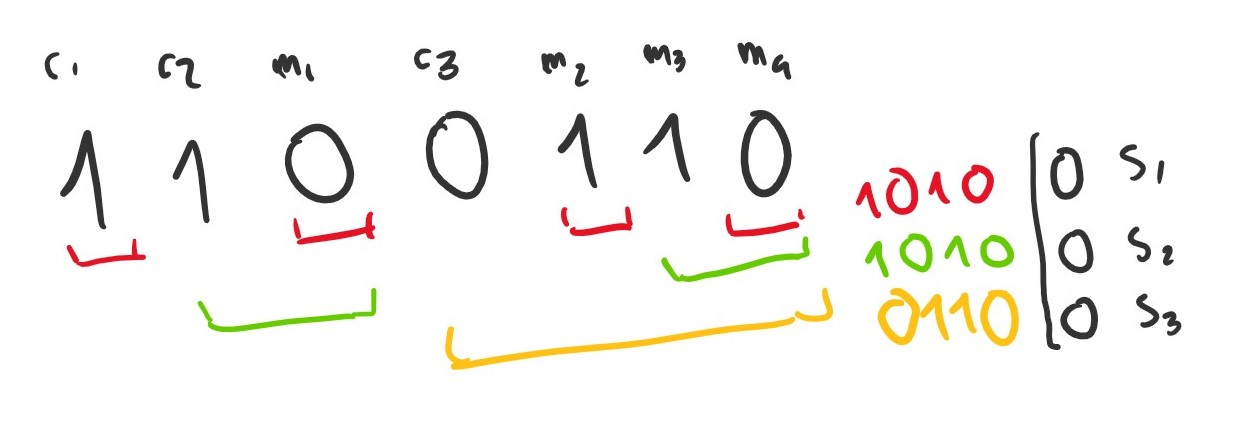
\includegraphics[width=0.7\linewidth]{immagini/img6}
\end{figure}

Quindi partendo dalla fine, il primo bit della sindrome viene calcolando facendo la parità sull'ultima cifra, terz'ultima e così via scalando sempre di 1, il secondo bit invece ne prende due alla volta e scala di due, il terzo ne prende quattro e scala di quattro. Seguendo sempre quindi lo schema di $2^n$.

\newpage

Se capitasse un errore?
Mettiamo che avvenga un errore in posizione 5, il messaggio passa da:

\begin{equation*}
1 \; 1 \; 0 \; 0 \; 1 \; 1 \; 0
\end{equation*}

a

\begin{equation*}
1 \; 1 \; 0 \; 0 \; \textbf{0} \; 1 \; 0
\end{equation*}

La cosa che farà il mittente sarà quindi quello di calcolare la sindrome.

\begin{equation*}
s_1 = \text{parity}(1000) = 1
\end{equation*}
\begin{equation*}
s_2 = \text{parity}(1010) = 0
\end{equation*}
\begin{equation*}
s_3 = \text{parity}(0010) = 1
\end{equation*}

Il valore finale sarà quindi $s_1 \; s_2 \; s_3$ uguale a 101, quindi il mittente riconosce che è avvenuto un errore in posizione 5.

E se la cifra modificata fosse di controllo? Proviamo con la seconda cifra:

\begin{equation*}
1 \; \textbf{0} \; 0 \; 0 \; 1 \; 1 \; 0
\end{equation*}

Calcolo della sindrome:

\begin{equation*}
s_1 = \text{parity}(1010) = 0
\end{equation*}
\begin{equation*}
s_2 = \text{parity}(0010) = 1
\end{equation*}
\begin{equation*}
s_3 = \text{parity}(0110) = 0
\end{equation*}

Quindi questo tipo di codici riconosce errori anche sulle cifre di controllo!
Ma nel caso di due errori nel messaggio? 
Proviamo a modificare due cifre del pacchetto:

\begin{equation*}
1 \; \textbf{0} \; 0 \; 0 \; \textbf{0} \; 1 \; 0
\end{equation*}

Calcolo della sindrome:

\begin{equation*}
s_1 = \text{parity}(1000) = 1
\end{equation*}
\begin{equation*}
s_2 = \text{parity}(0010) = 1
\end{equation*}
\begin{equation*}
s_3 = \text{parity}(0010) = 1
\end{equation*}

Essa dice che è avvenuto un errore in posizione 7, cosa falsa.
Si noti quindi come il codice di Hamming copre un singolo errore, nel caso di errori multipli essi non sono riconoscibili.

\newpage 

Come si gestisce il caso di 4 cifre di controllo?

\begin{equation*}
m=4
\end{equation*}
\begin{equation*}
2^m \geq n+1
\end{equation*}
\begin{equation*}
16 \geq n+1
\end{equation*}
\begin{equation*}
n \leq 15
\end{equation*}
\begin{equation*}
n = 15 \; (\text{ottimale})
\end{equation*}
\begin{equation*}
k=n-m=15-4=11
\end{equation*}

Vediamo come si distribuiscono le cifre di controllo nel messaggio:

\begin{table}[h]
	\centering
	\begin{tabular}{|l|l|l|l|l|l|l|l|l|l|l|l|l|l|l|}
		\hline
		$c_1$ & $c_2$ & $m_1$ & $c_3$ & $m_2$ & $m_3$ & $m_4$ & $c_4$ & $m_5$ & $m_6$ & $m_7$ & $m_8$ & $m_9$ & $m_{10}$ & $m_{11}$ \\
		\hline
		1   & 2   & 3   & 4   & 5   & 6   & 7   & 8   & 9   & 10  & 11  & 12  & 13  & 14   & 15  \\
		\hline
	\end{tabular}
\end{table}

Come si calcolano i bit di controllo? Come prima:

\begin{equation*}
c_1 \oplus m_1 \oplus m_2 \oplus m_4 \oplus m_5 \oplus m_7 \oplus m_9 \oplus m_{11} = 0
\end{equation*}
\begin{equation*}
c_2 \oplus m_1 \oplus m_3 \oplus m_4 \oplus m_6 \oplus m_7 \oplus m_{10} \oplus m_{11} = 0
\end{equation*}
\begin{equation*}
c_3 \oplus m_2 \oplus m_3 \oplus m_4 \oplus m_8 \oplus m_9 \oplus m_{10} \oplus m_{11} = 0
\end{equation*}
\begin{equation*}
c_4 \oplus m_5 \oplus m_6 \oplus m_7 \oplus m_8 \oplus m_9 \oplus m_{10} \oplus m_{11} = 0
\end{equation*}

\subsection*{Codici di Hamming ottimali}
\addcontentsline{toc}{subsection}{Codici di Hamming ottimali}
Come si può dedurre da quello spiegato sopra, i codici di Hamming definiti "ottimali" sono quelli che utilizzano tutte le configurazioni della sindrome sono utilizzate.
Questo equivale a dire che:
\begin{equation}
2^m=n+1
\end{equation}
Isolando la \textit{n}, si ottiene che $n = 2^m-1$. Questo per mostrare che i codici ottimali hanno sempre un numero di bit totali uguale a una potenza di 2 meno uno (3, 7, 15, 31, 63, 127...).
Quando vale la ridondanda dei codici di Hamming ottimali?

\begin{equation}
R = \frac{n}{k}
\end{equation}
\begin{equation*}
R = \frac{k+m}{k}
\end{equation*}
\begin{equation*}
R = 1 + \frac{m}{k}
\end{equation*}

Qual è la relazione fra \textit{k} e \textit{m}? Per i codici quadrati, cubici, ecc abbiamo notato un rapporto polinomiale.

\begin{equation*}
2^m=m+k+1
\end{equation*}
\begin{equation*}
2^m-m-1 = k
\end{equation*}
A sinistra prevale $2^m$, quindi:
\begin{equation*}
2^m \approx k
\end{equation*}

Per cui possiamo riscrivere la ridondanza in questo modo:
\begin{equation*}
R = 1 + \frac{m}{2^m}
\end{equation*}
oppure
\begin{equation*}
R = 1 + \frac{log_2k}{k}
\end{equation*}
Che decresce esponenzialmente.

I casi limite di questo tipo di codici sono $m=2$ (2 cifre di controllo e 1 di messaggio) e $m=1$ (1 cifra di controllo), cosa che deriva dal fatto che le funzioni esponenziali crescono inizialmente in modo lento, e poi esplodono.
Più sono lunghi i pacchetti, più le cifre di controllo sono "dilatate" nel messaggio (all'inizio adiacenti [$2^0 - 1$], poi staccate di 1 [$2^1 - 1$], poi di 3 [$2^2 - 1$], poi di 7 [$2^3 - 1$] e così via).

\subsubsection*{Caso particolare - Codici di Hamming a 2 cifre}
Nonostante possano sembrare molto ridondanti, i codici di Hamming a due cifre di controllo possono avere un'applicazione efficace.
In questo caso la banda del canale viene utilizzata solo a $\frac{1}{3}$ della sua disponibilità in quanto per mandare un bit ne invio un totale di 3, in particolare invio 000 per inviare 0, 111 per inviare 1.

Su uno Space Shuttle, le possibilità di errore sono tante (raggi solari, temperature ecc), tutti i componenti sono triplicati. 
Se un pacchetto arriva con 0 e con 1 (esempio, arriva 001) allora si ragiona in probabilità, come si è visto in precedenza la probabilità che avvengano due errori (nel modello di rumore bianco), è moolto più bassa di quella che avvenga un errore solo. Quindi per decodificare si fa osserva quale bit è più "usato", ad esempio se arriva 101 allora viene decodificato come 1, 001 come 0, 100 come 0 e così via.


\newpage
\section*{Lezione 5}
\addcontentsline{toc}{section}{Lezione 5}

\subsection*{Intepretazione geometrica}
\addcontentsline{toc}{subsection}{Interpretazione geometrica}
\subsubsection*{Cubi}
\addcontentsline{toc}{subsubsection}{Cubi}

Abbiamo detto che l'insieme $<\{0, 1\}^n, +_2, \cdot>$ è uno spazio vettoriale.
Supponiamo di avere $n=3$, quindi dal canale entrano ed escono vettori di 3 bit.
Diciamo che ognuno di questi bit rappresenta un lato di un cubo in tre dimensioni, successivamente "appoggiamo" questo cubo all'interno di uno spazio come ${\rm I\!R^3}$.

\begin{figure}[h]
	\centering
	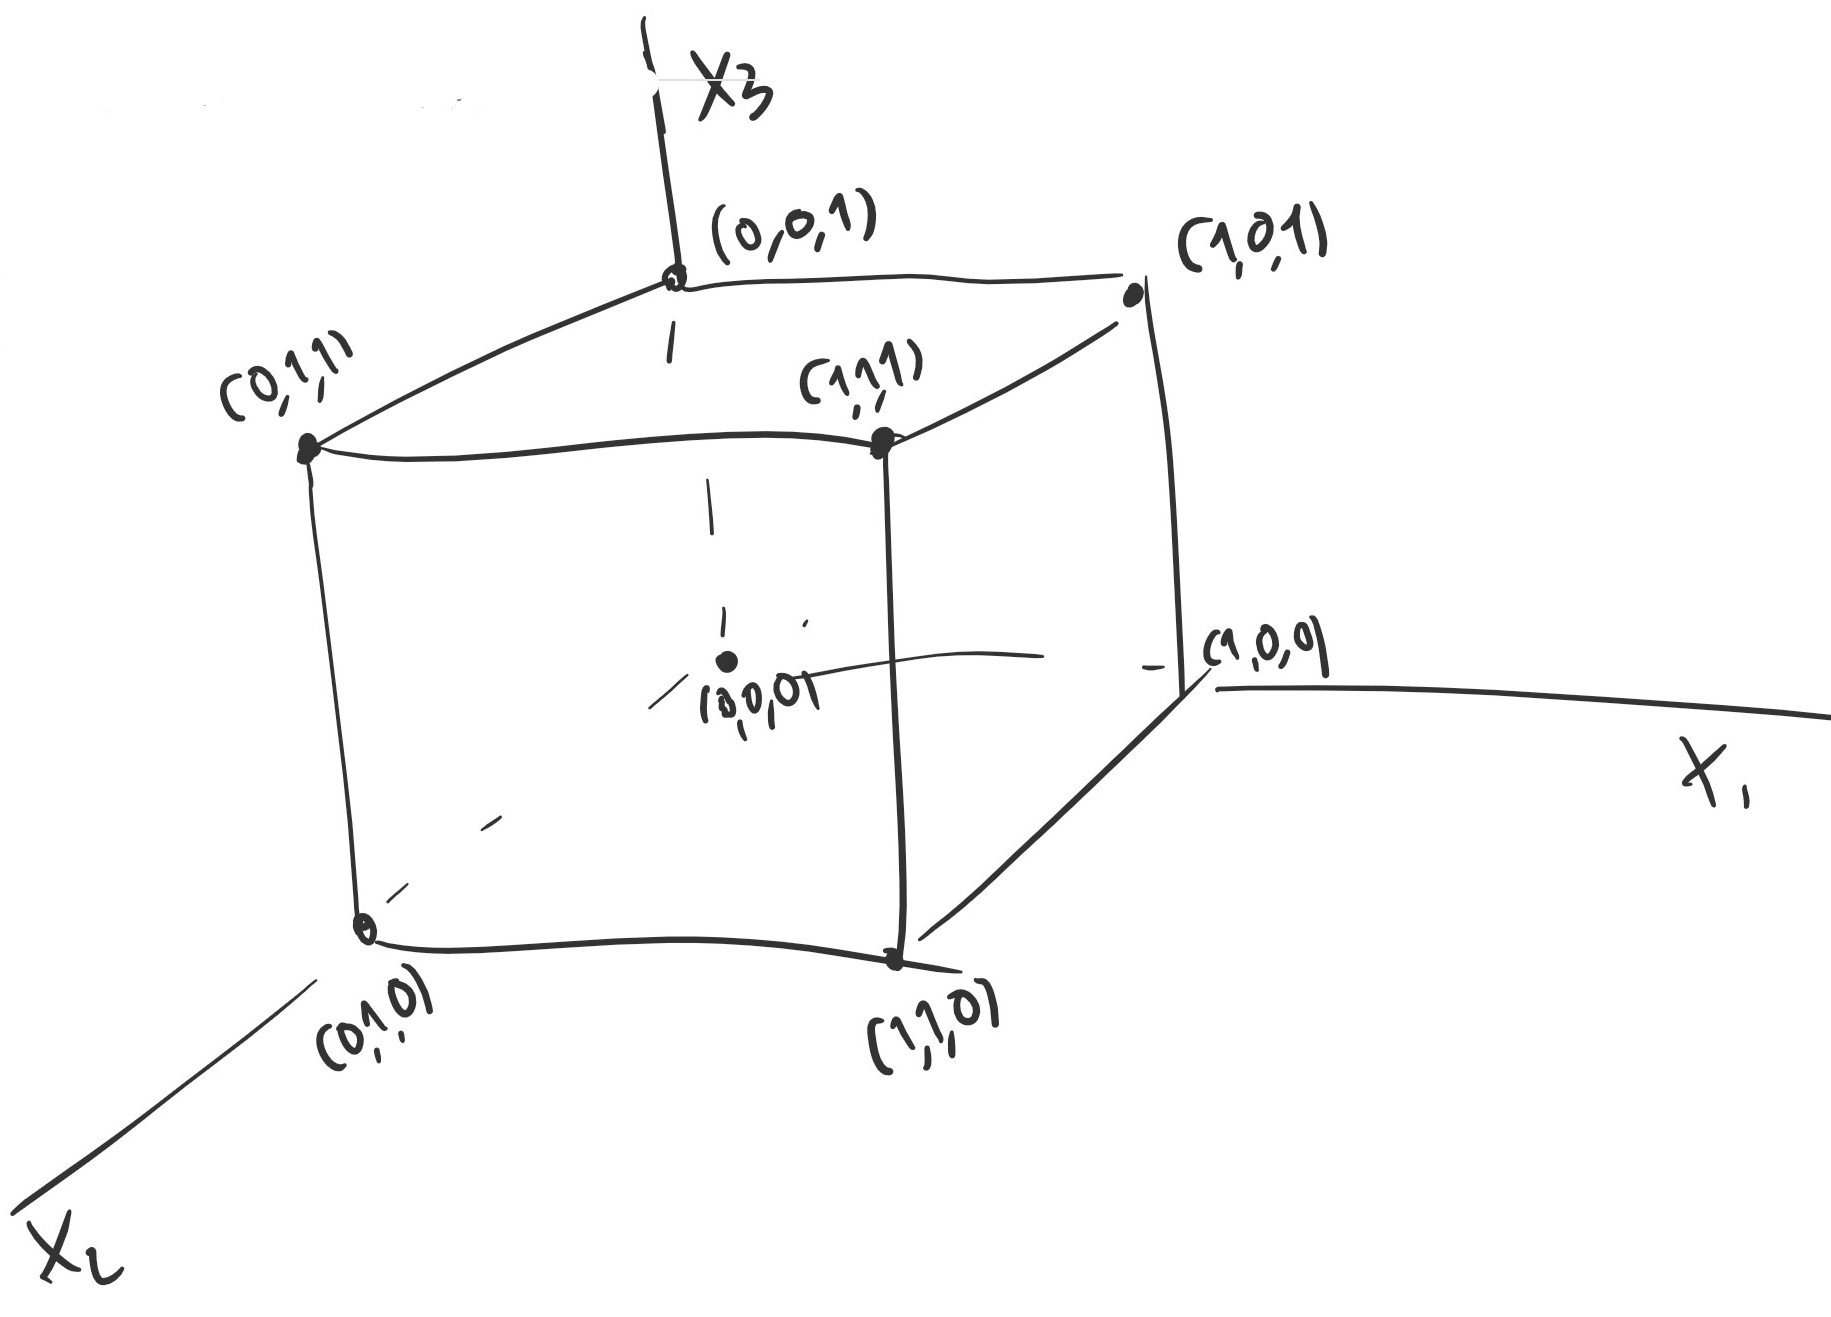
\includegraphics[width=0.7\linewidth]{immagini/img7}
\end{figure}

L'origine corrisponderà al messaggio (0, 0, 0), ogni asse rappresenterà quindi un bit.

L'idea è ovviamente utilizzabile in \textit{n} dimensione, usando quindi dei cubi di \textit{n} dimensioni.

I vertici del cubo rappresentano quindi tutte le possibile sequenze di messaggi. Un sottoinsieme di questi vettori, o vertici, rappresenta i messaggi "validi", quindi senza errore.
Ma cosa vuol dire dal punto di vista geometrico che un messaggio non è valido?
Supponiamo di mandare un messaggio 010, e che il rumore lo trasformi in 011. Un errore significa che ci siamo "mossi" da un vertice ad un altro del cubo. Un errore alla prima posizione ci fa muovere lungo l'asse $x_1$, un errore alla seconda posizione lungo l'asse $x_2$ e così via.

Il mittente e il destinatario devono quindi mettersi d'accordo su quali vertici siano "accettabili".

Mettiamo che i vertici accettabili siano 011 e 111

\begin{figure}[H]
	\centering
	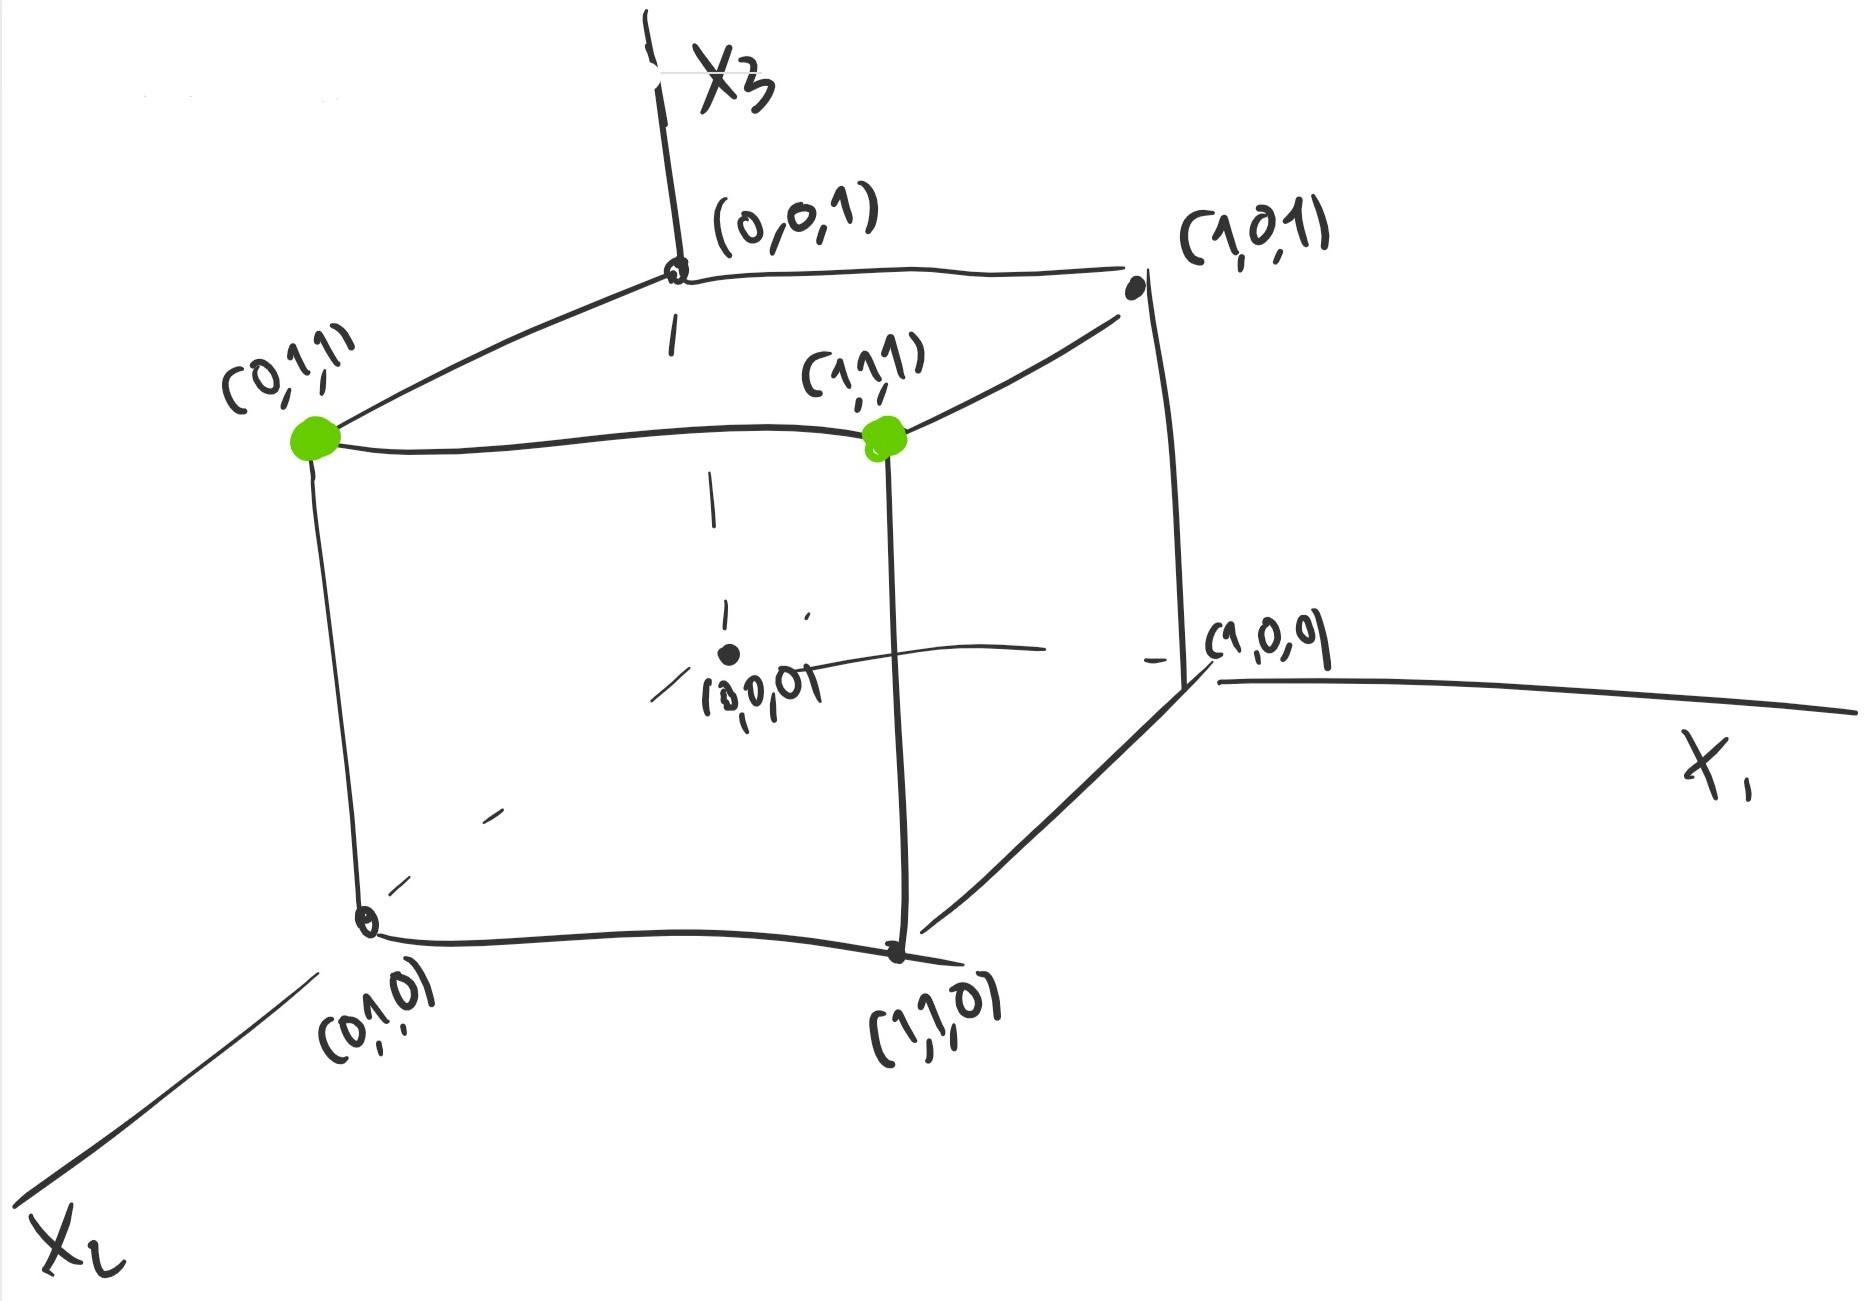
\includegraphics[width=0.7\linewidth]{immagini/img8}
\end{figure}


Ora mettiamo che nel canale il messaggio da 011 si sposti lungo la direzione $x_1$, quindi il messaggio diventa 111. Esso è accettabile però!

Definiamo la distanza di Hamming: dati due vettori \textit{u} e \textit{v} come il numero che bit che bisogna cambiare in \textit{u} per ottenere \textit{v} (e viceversa).

Ad esempio la distanza di Hamming fra 011 e 111 è 1.

Possiamo definire questa distanza anche usando la somma bit a bit.
$(0,1,1) \oplus (1,1,1) = (1,0,0)$
La distanza di Hamming è uguale a:
\begin{equation}
d_H(u)=\sum_{i=1}^{n}u_i
\end{equation}
Che rappresenta il numero di 1 all'interno dello xor bit a bit fra i due vettori.

Tornando al nostro cubo, diciamo che due vertici adiacenti non possono essere entrambi validi visto che, a causa di un errore, ci si sposta da uno all'altro; il mittente non rileverà l'errore!

Se nel mio codice la distanza di Hamming fra codici valdi è uguale a 1, non riuscirò mai a riconoscere errori.

Il numero di "passi" che devo fare da un vertice all'altro del cubo è uguale alla distanza di Hamming che c'è fra i due valori rappresentati dai vertici.

Se selezionassi le parole valide usando distanza di Hamming = 2?
Posso vedere la distanza fra i vertici in questo modo:

\begin{figure}[H]
	\centering
	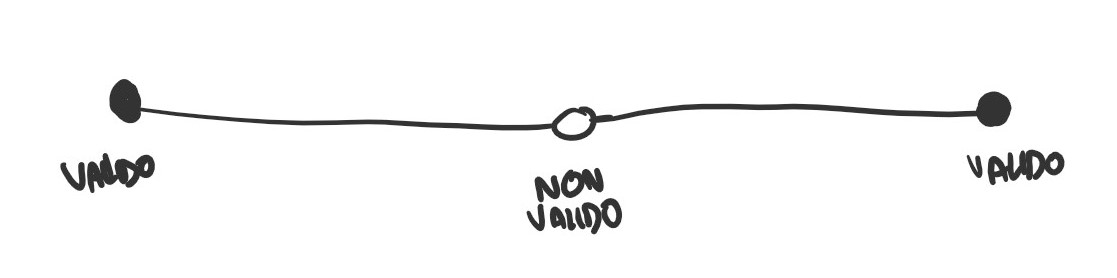
\includegraphics[width=0.7\linewidth]{immagini/img9}
\end{figure}
Nel caso di errore singolo, il messaggio inviato si "sposterebbe" in un vertice adiacente (quindi con distanza di Hamming = 1) che però non verrà accettato dal mittente (visto che i validi sono a distanza 2).

E per quanto riguarda distanza di Hamming = 3?

\begin{figure}[H]
	\centering
	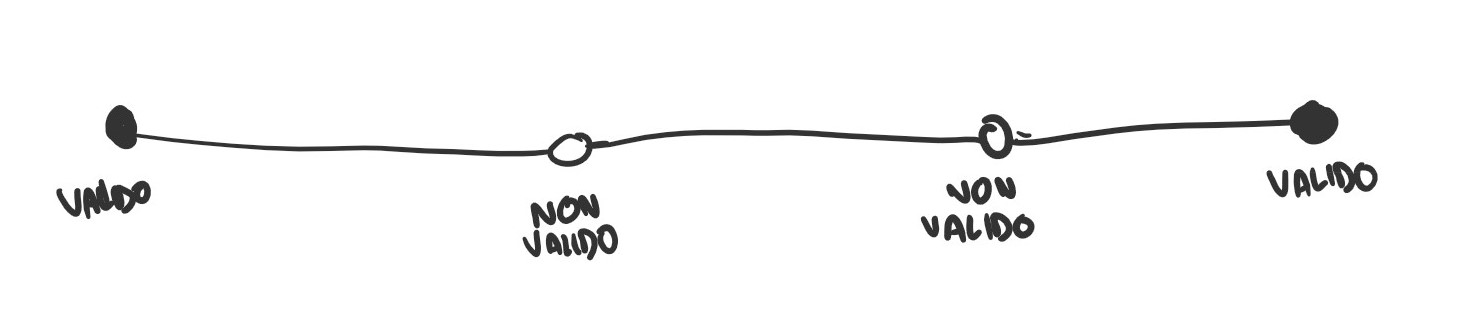
\includegraphics[width=0.7\linewidth]{immagini/img10}
\end{figure}

Nel caso di errore singolo, ci si sposterebbe in questo modo:

\begin{figure}[H]
	\centering
	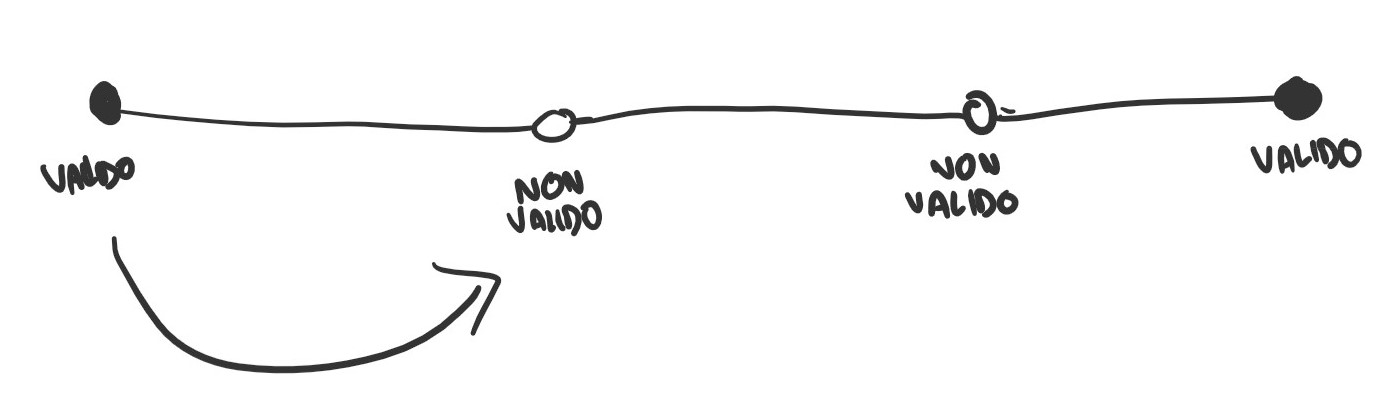
\includegraphics[width=0.7\linewidth]{immagini/img11}
\end{figure}

A questo punto il mittente si chiede: è più probabile che il messaggio arrivi dal vertice a sinistra (con un errore) o dal vertice di destra (con due errori)? Ovviamente è più probabile il vertice sinistro, quindi con questa distanza posso rilevare l'errore e anche correggerlo.
Nel caso di due errori, però, il ricevente sbaglierebbe a correggere l'errore; seguendo l'esempio precedente andrebbe al vertice destro.

Vediamo quindi anche il caso di distanza di Hamming = 4:

\begin{figure}[H]
	\centering
	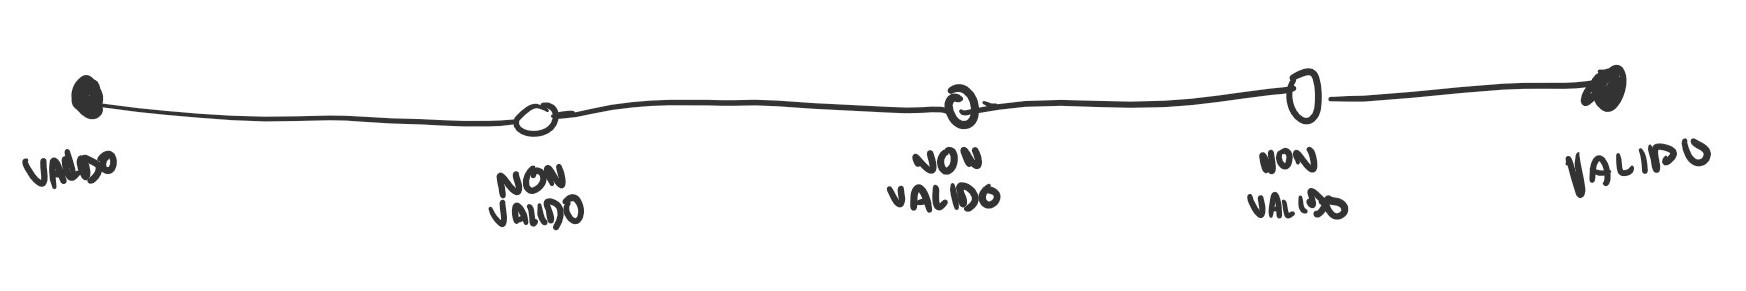
\includegraphics[width=0.7\linewidth]{immagini/img12}
\end{figure}

\'E facile notare come si può correggere facilmente un errore, ma in caso di errore doppio ci si troverà ad un punto equidistante dai due estremi (ovviamente nel caso di tre errori se ne introdurrà un quarto correggendo in maniera sbagliata).

E così via, riassumiamo il tutto con questa tabella:

\begin{table}[h]
	\centering
	\begin{tabular}{l|l|l}
		$d_H$ & errori rilevati & errori corretti \\
		\hline
		1     & 0               & 0               \\
		2     & 1               & 0               \\
		3     & 1               & 1               \\
		4     & 2               & 1               \\
		5     & 2               & 2              \\
		\vdots & \vdots & \vdots
	\end{tabular}
\end{table}

\newpage

\subsubsection*{Sfere}
\addcontentsline{toc}{subsubsection}{Sfere}
Proviamo a cambiare punto di vista, riprendiamo la rappresentazione su segmenti:

%dis

Immaginiamo che il messaggio valido inserito nel canale sia il centro di una sfera.
Se il messaggio che esce fa parte di un unica sfera, lo si può correggere "riportandolo" al centro della sfera. Se invece il messaggio fa parte di più sfere, rilevo l'errore ma non so a quale centro appartenga.

%disegni esempi

Ma come definisco una sfera nello spazio vettoriale? Dico che la sfera \textit{S} è
\begin{equation}
S(x,r) = \{y \in \{0,1\}^n | d_H(x,y) \leq r \}
\end{equation}

Possiamo vedere l'effetto degli errori come una somma xor:

\begin{equation*}
(1,1,0) \oplus (0,1,0) = (1,0,0)
\end{equation*}

In questo caso è avvenuto un posizione 2, quindi è come sommare un vettore con un 1 in posizione 2.

Se capissi qual è il vettore errore mi basterebbe ri-sommarla, per ottenere il messaggio di partenza:

\begin{equation*}
(1,1,0) \oplus (0,1,0) = (1,0,0)
\end{equation*}
\begin{equation*}
(1,0,0) \oplus (0,1,0) = (1,1,0)
\end{equation*}

Riconsideriamo i codici di Hamming con distanza 3, quindi a rilevamento e correzione d'errore singolo.
Ci chiediamo quanto vale il volume della sfera centrata nel vettore che inviamo di raggio 1.

\begin{equation}
V(S(x,1))=1+n
\end{equation}

In generale:

\begin{equation*}
V(S(x,r))=1+n+\binom{n}{2} + \binom{n}{3} + \dots \binom{n}{r}
\end{equation*}
\begin{equation}
V(S(x,r))= \sum_{i=0}^r \binom{n}{i}
\end{equation}

Quanti messaggi validi posso creare in questo modo?
Data distanza di Hamming $d_H=3$, messaggi di \textit{n} bit, quindi uno spazio grande $2^n$ e $n$ sfere grandi $(n+1)$, dico che:

\begin{equation}
\frac{\text{volume spazio}}{\text{volume sfera}} \geq \text{numero massimo di sfere / messaggi}
\end{equation}

\newpage

Applicato al nostro esempio:

\begin{equation*}
\frac{2^n}{n+1} \geq 2^k \; \; \; \; \; \; \; n = k + m
\end{equation*}
\begin{equation*}
2^n \geq 2^k(n+1)
\end{equation*}
\begin{equation*}
\cancel{2^k} 2^m \geq \cancel{2^k}(n+1)
\end{equation*}
\begin{equation*}
2^m \geq n+1
\end{equation*}
Che è la stessa conclusione a cui è arrivato Hamming per i codici ottimali!

\subsection*{Codifica di sorgente}
\addcontentsline{toc}{subsection}{Codifica di sorgente}

L'obiettivo della codifica di sorgente è quello di creare delle codeword ottimali, ad esempio codificando con codeword più piccole i caratteri più utilizzati (codice morse).

Ci sono diversi codici per la codifica di sorgente, distinguibili in due:
\begin{itemize}
	\item Codici a blocchi: tutte le codeword hanno la stessa lunghezza ($\ell_1 = \ell_2 = ... = \ell_q$)
	\begin{itemize}
		\item Vantaggi: il ricevente ha 'vita facile' per decodificare in quanto sa subito quando inizia e quando finisce la codeword (sa già la lunghezza)
		\item Svantaggi: se un simbolo esce con probabilità alta, allora abbiamo un grande spreco (uso gli stessi bit che userei con un simbolo usato raramente)
	\end{itemize}
La lunghezza media delle codeword ($\sum_{i=1}^qp_i = 1$) è ovviamente:
\begin{equation}
L=\sum_{i=1}^q+p_i\ell_i = \sum_{i=1}^qp_i\ell = \ell \sum_{i=1}^qp_i = \ell
\end{equation}
uguale per tutti.
Questo tipo di codice conviene quando la distribuzione delle probabilità per i simboli di uscire è uniforme.
\item Lunghezza variabile: le codeword hanno lunghezze diverse, di solito i caratteri che escono con probabilità $p_i$ maggiori sono codificati in codeword più brevi. 
\begin{itemize}
	\item Vantaggi: C'è meno spreco di spazio, le codeword si adattano alle probabilità dei simboli
	\item Svantaggi: Per il ricevente non è semplice capire quando una codeword finisce.
\end{itemize}
A causa di questo svantaggio si introducono due sottoclassi dei codici a lunghezza variabile:
\begin{itemize}
	\item Univocamente decodificabili: quando il ricevente riceve una sequenza di codeword (es $w_1, w_2 \dots w_k$) di lunghezza diversa, allora esiste un unico modo di spezzare la sequenza di codeword
	\item Non univocamente decodificabili: al contrario, non esiste un unico modo di spezzare la sequenza ricevuta (ad esempio posso spezzare una sequenza sia in $s_1s_1s_2$ che in $s_3s_2$).
\end{itemize}
Nel corso useremo \textbf{solo} codici univocamente decodificabili.
\end{itemize}










\newpage
\section*{Lezione 6}
\addcontentsline{toc}{section}{Lezione 6}

Cominciamo con un esempio: supponiamo di avere una sorgente caratterizzata da quattro simboli, codificati in questo modo:

\begin{equation*}
s_1 \rightarrow 0
\end{equation*}
\begin{equation*}
s_2 \rightarrow 01
\end{equation*}
\begin{equation*}
s_3 \rightarrow 11
\end{equation*}
\begin{equation*}
s_4 \rightarrow 00
\end{equation*}

A questo punto supponiamo che il ricevente riceva la stringa 0011, qual è la sequenza di codeword che ho ricevuto?
Una soluzione potrebbe essere $s_1, s_1, s_3$, ma anche $s_4, s_3$.
Questa codifica e questa sequenza mette in crisi il ricevitore, ed è uno dei casi da evitare (non univocamente decodificabile).


Tra i codici \textbf{univocamente decodificabili} possiamo distinguere due ulteriori sottocasi:
\begin{itemize}
	\item Istantanei: il ricevente appena finito di ricevere una codeword la decodifica senza ambiguità.
	\item Non istantantei: non vale la regola precedente.
\end{itemize}

Vediamo un esempio di codice univocamente decodificabile \underline{non istantaneo}:

\begin{equation*}
s_1 \rightarrow 0
\end{equation*}
\begin{equation*}
s_2 \rightarrow 01
\end{equation*}
\begin{equation*}
s_3 \rightarrow 011
\end{equation*}
\begin{equation*}
s_4 \rightarrow 111
\end{equation*}

Immaginiamo di dover decodificare la sequenza 011111111, all'inizio potrei star leggendo $s_1, s_2, s_3$, dipende da cosa arriva dopo. 
Dopo arriva 1, e anche qui c'è ambiguità fra $s_2$ e $s_3$, e così via.

Partendo dal fondo però, quando la trasmissione è finita, si può decodificare il messaggio partendo dalla fine:
\begin{equation*}
011 \; \; 111 \; \; 111
\end{equation*}
\begin{equation*}
s_3 \; \; s_4 \; \; s_4
\end{equation*}

Il lato negativo è che devo attendere la fine della trasmissione per decodificare il messaggio.
I codici istantanei invece, non sono caratterizzati da questa pecca.
Un codice istantaneo implica che \textbf{nessuna codeword è prefissa di un'altra}.
Nel codice di prima, $s_1$ è prefisso di $s_2$, ecc.

\newpage
Vediamo questo esempio:

\begin{equation*}
s_1 \rightarrow 0
\end{equation*}
\begin{equation*}
s_2 \rightarrow 10
\end{equation*}
\begin{equation*}
s_3 \rightarrow 110
\end{equation*}
\begin{equation*}
s_4 \rightarrow 111
\end{equation*}

E decodifichiamo 1011001110 ($s_2, s_3, s_1, s_4, s_1$) si noti come partendo dall'inizio si può riconoscere immediatamente le codeword, senza attendere il ricevimento della sequenza completa.

\subsection*{Albero di decodifica}
\addcontentsline{toc}{subsection}{Albero di decodifica}

Il lavoro del ricevente per codificare si può rappresentare con un albero di decodifica.
All'inizio egli si trova alla radice dell'albero, poi si sposta all'interno di esso seguendo i simboli sulle freccie:


\begin{figure}[H]
\centering
\vspace{4mm}
\begin{tikzpicture}
[
grow                    = right,
sibling distance        = 6em,
level distance          = 7em,
edge from parent/.style = {draw, -latex},
every node/.style       = {font=\footnotesize},
sloped
]
\node [root] {}
child { node [dummy] {}
		child { node [dummy] {}
			child { node [dummy] {$s_4$}
				edge from parent node [below] {1}}
			child { node [dummy] {$s_3$}
				edge from parent node [above] {0}}
			edge from parent node [below] {1}}
		child { node [dummy] {$s_2$}
			edge from parent node [above] {0}}
	edge from parent node [below] {1}}
child { node [dummy] {$s_1$}
	edge from parent node [above] {0}
	 };
\end{tikzpicture}
\caption{Albero di decodifica per $s_1 \rightarrow 0$, $s_2 \rightarrow 10$, $s_3 \rightarrow 110$, $s_4 \rightarrow 111$}
\end{figure}
Questa rappresentazione è molto utile in quanto si riconosce immediatamente l'istantaneità dei codici istantanei, inoltre è possibile passare dall'albero di decodifica al codice e viceversa.

Un albero è definito vuoto oppure un nodo che punta ad altri alberi (ovviamente in termini ricorsivi).

\newpage

Un'altra cosa da notare è che gli alberi di decodifica sono utilizzabili solo per codici istantanei, cosa succede se non lo sono?
Proviamo con:


\begin{equation*}
s_1 \rightarrow 0
\end{equation*}
\begin{equation*}
s_2 \rightarrow 01
\end{equation*}
\begin{equation*}
s_3 \rightarrow 011
\end{equation*}
\begin{equation*}
s_4 \rightarrow 111
\end{equation*}

\begin{figure}[H]
	\centering
	\vspace{4mm}
	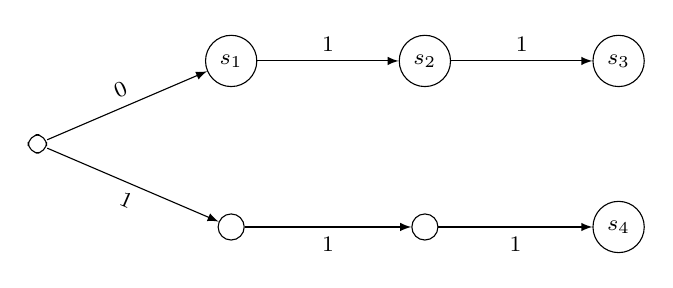
\begin{tikzpicture}
	[
	grow                    = right,
	sibling distance        = 6em,
	level distance          = 7em,
	edge from parent/.style = {draw, -latex},
	every node/.style       = {font=\footnotesize},
	sloped
	]
	\node [root] {}
	child { node [dummy] {}
		child { node [dummy] {}
			child { node [dummy] {$s_4$}
				edge from parent node [below] {1}}
					edge from parent node [below] {1}}
		edge from parent node [below] {1}}
	child { node [dummy] {$s_1$}
		child { node [dummy] {$s_2$}
			child { node [dummy] {$s_3$}
				edge from parent node [above] {1}}
			edge from parent node [above] {1}}
		edge from parent node [above] {0}
	};
	\end{tikzpicture}
	\caption{Albero di decodifica per $s_1 \rightarrow 0$, $s_2 \rightarrow 01$, $s_3 \rightarrow 011$, $s_4 \rightarrow 111$, codice non istantaneo}
\end{figure}

Si nota facilmente come durante il ricevimento non si può stabilire univocamente a che $s_i$ si sta facendo riferimento (una codifica non deterministica, o megllio, lo diventa solo alla fine).

L'esempio di codice istantaneo di prima, $s_1 \rightarrow 0$, $s_2 \rightarrow 10$, $s_3 \rightarrow 110$, $s_4 \rightarrow 111$ è chiamato \textbf{comma code}, in quanto il messaggio termina o quanto arrivano tre 1 oppure quando arriva uno 0. Il relativo albero verrà disegnato "a pettine".

Vediamo un altro esempio di comma code a cinque codeword:

\begin{equation*}
s_1 \rightarrow 0
\end{equation*}
\begin{equation*}
s_2 \rightarrow 10
\end{equation*}
\begin{equation*}
s_3 \rightarrow 110
\end{equation*}
\begin{equation*}
s_4 \rightarrow 1110
\end{equation*}
\begin{equation*}
s_5 \rightarrow 1111
\end{equation*}

\begin{figure}[H]
	\centering
	\vspace{4mm}
	\begin{tikzpicture}
	[
	grow                    = right,
	sibling distance        = 6em,
	level distance          = 7em,
	edge from parent/.style = {draw, -latex},
	every node/.style       = {font=\footnotesize},
	sloped
	]
	\node [root] {}
	child { node [dummy] {}
		child { node [dummy] {}
			child { node [dummy] {}
				child { node [dummy] {$s_5$}
					edge from parent node [below] {1}}
				child { node [dummy] {$s_4$}
					edge from parent node [above] {0}}
				edge from parent node [below] {1}}
			child { node [dummy] {$s_3$}
				edge from parent node [above] {0}}
			edge from parent node [below] {1}}
		child { node [dummy] {$s_2$}
			edge from parent node [above] {0}}
		edge from parent node [below] {1}}
	child { node [dummy] {$s_1$}
		edge from parent node [above] {0}
	};
	\end{tikzpicture}
	\caption{Albero di decodifica per $s_1 \rightarrow 0$, $s_2 \rightarrow 10$, $s_3 \rightarrow 110$, $s_4 \rightarrow 1110$, $s_5 \rightarrow 1111$}
\end{figure}

Vediamo ora un altro esempio (non comma code):

\begin{equation*}
s_1 \rightarrow 00
\end{equation*}
\begin{equation*}
s_2 \rightarrow 01
\end{equation*}
\begin{equation*}
s_3 \rightarrow 10
\end{equation*}
\begin{equation*}
s_4 \rightarrow 110
\end{equation*}
\begin{equation*}
s_5 \rightarrow 111
\end{equation*}

\begin{figure}[H]
	\centering
	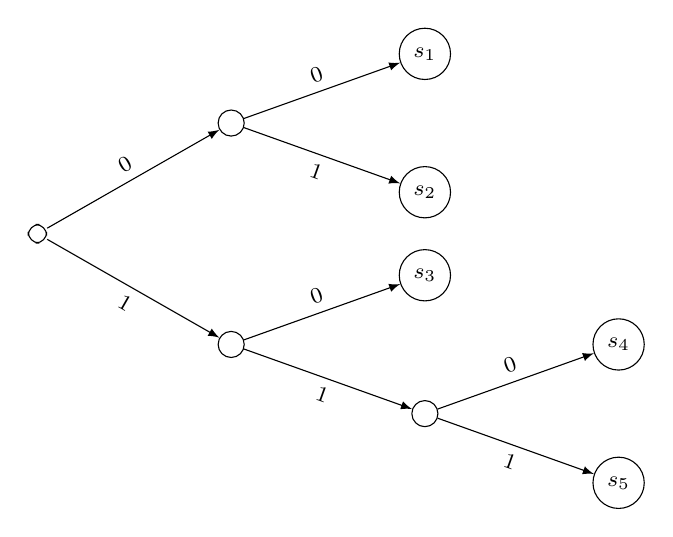
\begin{tikzpicture}
	[
	grow                    = right,
	level 1/.style={sibling distance=8em},
	level 2/.style={sibling distance=5em},
	level distance          = 7em,
	edge from parent/.style = {draw, -latex},
	every node/.style       = {font=\footnotesize},
	sloped
	]
	\node [root] {}
	child { node [dummy] {}
		child { node [dummy] {}
			child { node [dummy] {$s_5$}
				edge from parent node [below] {1}}
			child { node [dummy] {$s_4$}
				edge from parent node [above] {0}}
			edge from parent node [below] {1}}
		child { node [dummy] {$s_3$}
			edge from parent node [above] {0}}
		edge from parent node [below] {1}}
	child { node [dummy] {}
		child { node [dummy] {$s_2$}
			edge from parent node [below] {1}}
		child { node [dummy] {$s_1$}
			edge from parent node [above] {0}}
		edge from parent node [above] {0}
	};
	\end{tikzpicture}
	\caption{Albero di decodifica per $s_1 \rightarrow 00$, $s_2 \rightarrow 01$, $s_3 \rightarrow 10$, $s_4 \rightarrow 110$, $s_5 \rightarrow 111$}
\end{figure}

Dopo aver definito queste due codifiche a cinque simboli, quale sarebbe da preferire?
Il criterio che utilizziamo è la lunghezza media, quindi senza sapere le probabilità dei simboli della sorgente non possiamo decidere a priori qual è più vantaggioso.\\
Supponiamo di avere queste probabilità: $p_1 = 0.9, \; p_2 = p_3 = p_4 = p_5 =  0.025$.
Andiamo quindi a calcolare le due lunghezze medie:
\begin{equation*}
L_{pettine} = 0.9 \cdot 1 + 0.025 \cdot 2 + 0.025 \cdot 3 + 0.025 \cdot 4 + 0.025 \cdot 4 = 1.225\frac{bit}{simbolo}
\end{equation*}

\begin{equation*}
L_{altroalbero} = 0.9 \cdot 2 + 0.025 \cdot 2 + 0.025 \cdot 2 + 0.025 \cdot 3 + 0.025 \cdot 3 = 2.05\frac{bit}{simbolo}
\end{equation*}

Quindi utilizzando questa distribuzione di probabilità il comma code è da preferire.
Usando la distribizione uniforme: $p_1 = p_2 = p_3 = p_4 = p_5 =  0.2$ avremo che:

\begin{equation*}
L_{pettine} = 0.9 \cdot 2 + 0.2 \cdot 2 + 0.2 \cdot 3 + 0.2 \cdot 4 + 0.2 \cdot 4 = 2.4\frac{bit}{simbolo}
\end{equation*}

\begin{equation*}
L_{altroalbero} = 0.2 \cdot 2 + 0.2 \cdot 2 + 0.2 \cdot 2 + 0.2 \cdot 3 + 0.2 \cdot 3 = 2.05\frac{bit}{simbolo}
\end{equation*}

La conclusione è che senza probabilità non possiamo trarre conclusioni sul tipo di albero da preferire per ottimizzare la lunghezza media delle codeword.


\subsection*{Disuguaglianza di Kraft}
\addcontentsline{toc}{subsection}{Disuguaglianza di Kraft}

Una domanda che potremmo porci è: quali sono le condizioni per cui posso costruire un codice istantaneo?

\begin{theorem}
Condizione necessaria e sufficiente affichè esista un codice istantaneo $r$-ario per una sorgente $S$ di $q$ simboli con codeword di lunghezze $\ell_1,\ell_2,...,\ell_q$ è che valga:
\begin{equation}
K = \sum_{i=1}^{q}\frac{1}{r^{\ell_i}} \leq 1
\end{equation}
\end{theorem}

Questo teorema \underline{non dice: questo è un codice istantaneo se e solo se...}, ma invece dice che esiste un codice istantaneo se e solo se...

L'utilità è la seguente: ho una sorgente con $q$ simboli, voglio costruire un codice istantaneo $r$-ario con codeword di lunghezze $\ell_1,\ell_2,...,\ell_q$, posso? Allora calcolo $K$ e vedo se il valore viene $\leq 1$

\newpage
\begin{dimostrazione}
La condizione necessaria e sufficiente richiede di dover dimostrare queste due cose:
\begin{itemize}
	\item Per ogni codice istantaneo $r$-ario per $q$ simboli e codeword di lunghezze $\ell_1,\ell_2,...,\ell_q$ $\rightarrow k\leq 1$
\end{itemize}
\begin{itemize}
	\item $k\leq 1 \rightarrow$ esiste codice istantaneo $r$-ario per $q$ simboli e codeword di lunghezze $\ell_1,\ell_2,...,\ell_q$
\end{itemize}

Partiamo dalla prima:\\
Utilizziamo come valore di $r=2$. Parlare di codici istantanei è uguale al considerare i relativi alberi di decodifica. Possiamo quindi dimostrare per induzione sulla profondità dell'albero.\\
\textbf{Caso base} (albero di decodifica di profondità 1)
I tre casi possibili sono i seguenti:
\begin{figure}[H]
	\centering
	\vspace{4mm}
	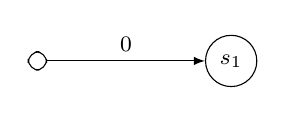
\begin{tikzpicture}
	[
	grow                    = right,
	sibling distance        = 6em,
	level distance          = 7em,
	edge from parent/.style = {draw, -latex},
	every node/.style       = {font=\footnotesize},
	sloped
	]
	\node [root] {}
	child { node [dummy] {$s_1$}
		edge from parent node [above] {0}
	};
	\end{tikzpicture}
\end{figure}
oppure
\begin{figure}[H]
	\centering
	\vspace{4mm}
	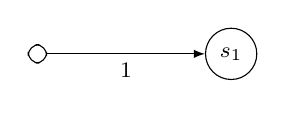
\begin{tikzpicture}
	[
	grow                    = right,
	sibling distance        = 6em,
	level distance          = 7em,
	edge from parent/.style = {draw, -latex},
	every node/.style       = {font=\footnotesize},
	sloped
	]
	\node [root] {}
	child { node [dummy] {$s_1$}
		edge from parent node [below] {1}
	};
	\end{tikzpicture}
\end{figure}
oppure
\begin{figure}[H]
	\centering
	\vspace{4mm}
	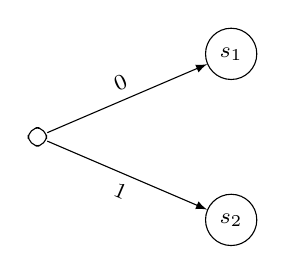
\begin{tikzpicture}
	[
	grow                    = right,
	sibling distance        = 6em,
	level distance          = 7em,
	edge from parent/.style = {draw, -latex},
	every node/.style       = {font=\footnotesize},
	sloped
	]
	\node [root] {}
	child { node [dummy] {$s_2$}
		edge from parent node [below] {1}}
	child { node [dummy] {$s_1$}
		edge from parent node [above] {0}};
	\end{tikzpicture}
\end{figure}

Andiamo quindi a calcolare i $K = \sum_{i=1}^{q}\frac{1}{r^{\ell_i}}$ dei tre alberi appena costruiti:
\begin{enumerate}
	\item $K=\frac{1}{2^1} = \frac{1}{2} \leq 1$
	\item $K=\frac{1}{2^1} = \frac{1}{2} \leq 1$
	\item $K=\frac{1}{2^1} + \frac{1}{2^1} = 1 \leq 1$
\end{enumerate}

Quindi per il passo base abbiamo dimostrato.\\

\newpage
\textbf{Passo induttivo}:\\
Supponiamo che il teorema valga per alberi di profondità $<n$ e dimostriamo che valga per alberi di profondità $n$ (dimostro per $<n$ e non $n-1$ perchè magari il sottoalbero sopra ha profondità 1, l'altro $n-1$, ma deve valere per entrambi).
La situazione è quindi la seguente:
\begin{figure}[h]
\centering
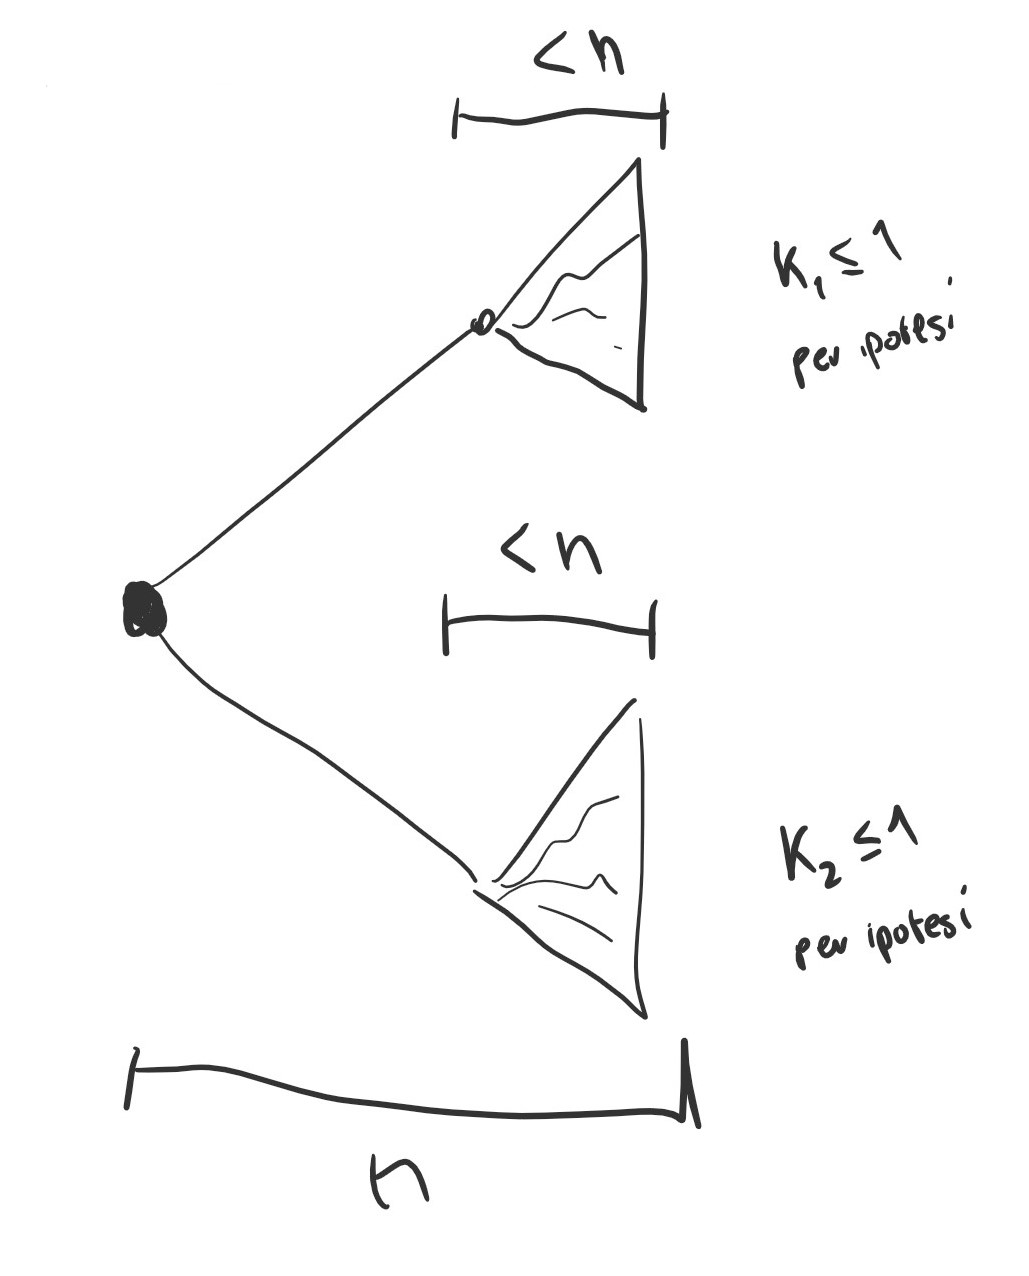
\includegraphics[width=0.45\linewidth]{immagini/img13}
\end{figure}


Quindi per ipotesi i due sottoalberi profondi al massimo $n-1$ hanno $K \leq 1$; supponendo di 'attaccarli' ad un nuovo nodo significa appendere come prefisso di tutte le codeword un altro simbolo.
\begin{figure}[h]
	\centering
	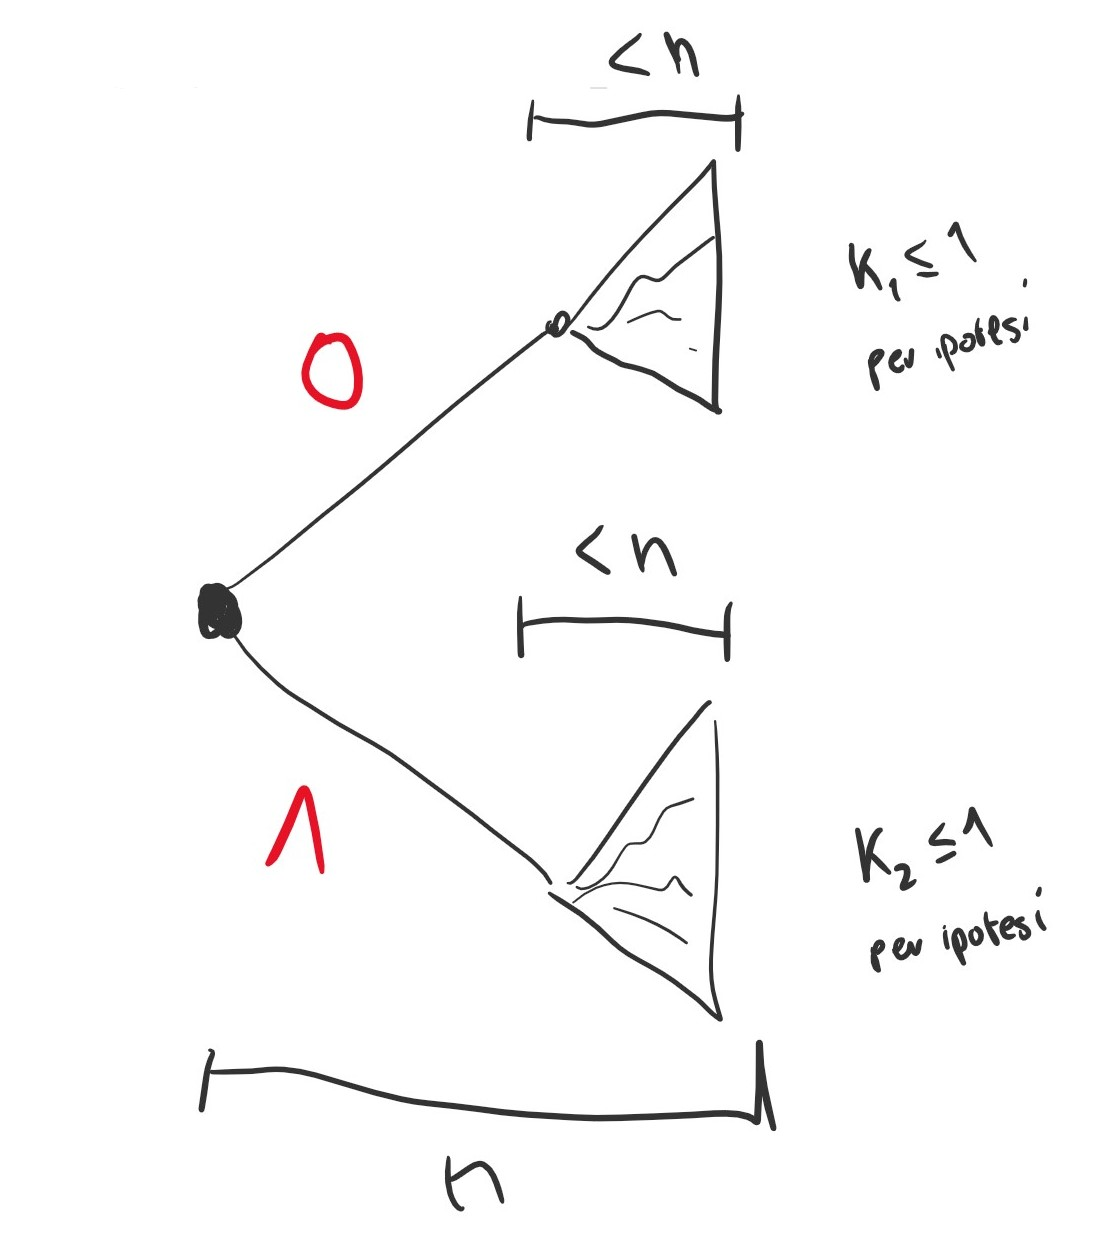
\includegraphics[width=0.45\linewidth]{immagini/img14}
\end{figure}

Come cambiano le $K$ quando allungo di uno le lunghezze delle codeword? Tutte le $\ell_i$ diventano $\ell_i + 1$:
\begin{equation*}
K_1 = \sum_{i=1}^{q}\frac{1}{r^{\ell_i+1}} = \sum_{i=1}^{q}(\frac{1}{r^{\ell_i}}\frac{1}{r}) = \frac{1}{r}\sum_{i=1}^{q}\frac{1}{r^{\ell_i}}
\end{equation*}

Quindi il contributo dato da ognuno dei due sottoalberi al calcolo di $K$ totale è dato da $\frac{1}{2}K_i$ (per $r=2$).
Il $K$ relativo all'albero totale quindi diventa:
\begin{equation*}
K = \frac{1}{2}K_1 + \frac{1}{2}K_2 = \frac{1}{2}(K_1 + K_2)
\end{equation*}
Sappiamo che $K_1 \leq 1$ e che $K_2 \leq 1$, quindi la loro somma sarà sicuramente $\leq 2$. La somma, moltiplicata per $\frac{1}{2}$ è $\leq 1$; quindi possiamo scrivere:
\begin{equation*}
K \leq 1
\end{equation*}
che è quello che volevamo dimostrare.\\

In caso $n$ non fosse $n=2$ bisogna solo creare più alberi di profondità 1 nel caso base:

\begin{figure}[H]
	\centering
	\vspace{4mm}
	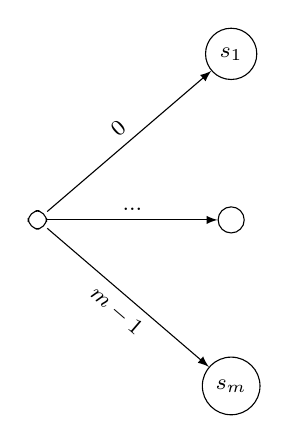
\begin{tikzpicture}
	[
	grow                    = right,
	sibling distance        = 6em,
	level distance          = 7em,
	edge from parent/.style = {draw, -latex},
	every node/.style       = {font=\footnotesize},
	sloped
	]
	\node [root] {}
	child { node [dummy] {$s_m$}
		edge from parent node [below] {$m-1$}}
	child { node [dummy] {}
		edge from parent node [above] {...}}
	child { node [dummy] {$s_1$}
		edge from parent node [above] {0}};
	\end{tikzpicture}
\end{figure}

Dato che $m \leq r$ (delle $r$ foglie possibili ne ha solo $m$)

\begin{equation*}
K=m(\frac{1}{r}) = \frac{m}{r} \leq 1
\end{equation*}

Nel passo induttivo il numero di sottoalberi sarà $m$, e quando attacchiamo i sottoalberi alla nuova radice il nuovo $K$ verrà
\begin{equation*}
K=\frac{1}{r}K_1+\frac{1}{r}K_2+...+\frac{1}{r}K_m
\end{equation*}

\newpage

Dimostriamo ora la seconda parte, ovvero "$k\leq 1 \rightarrow$ esiste codice istantaneo $r$-ario per $q$ simboli e codeword di lunghezze $\ell_1,\ell_2,...,\ell_q$".

Partiamo dall'ipotesi che $K \leq 1$, successivamente definiamo $\ell$ come:
\begin{equation*}
\ell = max\{\ell_1, \ell_2,...,\ell_q\}
\end{equation*}
Inoltre chiamo $t_j$ il numero di codeword di lunghezza $j$.

Riscriviamo $K$ in questo modo:
\begin{equation*}
K = \sum_{i=1}^{q}\frac{1}{r^{\ell_i}} = \sum_{i=1}^{\ell}t_i\cdot\frac{1}{r^i}
\leq 1
\end{equation*}
Posso riscriverlo in questo modo perchè è come se stessi raccogliendo le codeword di lunghezza uguale $t_i$.
Moltiplico per $r^\ell$ entrambi i membri:
\begin{equation*}
\sum_{i=1}^{\ell}t_ir^{\ell-1} \leq r^\ell
\end{equation*}
Questo equivale a:
\begin{equation*}
	t_1r^{\ell-1}+t_2r^{\ell-2}+..+t_{\ell-1}r+t_\ell \leq r^\ell
\end{equation*}
Isolo $t_\ell$:
\begin{equation*}
t_\ell \leq r^{\ell} -t_1r^{\ell-1}-t_2r^{\ell-2}-...-t_{\ell-1}r
\end{equation*}
So che $t_\ell$ è maggiore o uguale a zero (numero di codeword di lunghezza $\ell$)
\begin{equation*}
0 \leq t_\ell \leq r^{\ell} -t_1r^{\ell-1}-t_2r^{\ell-2}-...-t_{\ell-1}r
\end{equation*}
Quindi ho posto un vincolo al numero massimo di codeword di lunghezza $\ell$. Ora considero solo questo pezzo:
\begin{equation*}
0 \leq r^{\ell} -t_1r^{\ell-1}-t_2r^{\ell-2}-...-t_{\ell-1}r
\end{equation*}
Divido tutto per $r$ e porto a sinistra l'ultimo termine $t_{\ell-1}r$:
\begin{equation*}
0 \leq t_{\ell-1} \leq r^{\ell-1} - t_1r^{\ell-2}-t_2r^{\ell-3}-...-t_{\ell-2}r
\end{equation*}
Posso rifarlo per tutti i $t$:
\begin{equation*}
0 \leq t_{\ell-2} \leq ...
\end{equation*}
E mi fermo a 
\begin{equation}
0 \leq t_2 \leq r^2-t_1r
\end{equation}
\begin{equation}
0 \leq t_1 \leq r \; \; \; \; \; \; \; \; \; \; \;
\end{equation}
Quindi sto ponendo dei limiti alle codeword di lunghezza 1, di lunghezza 2, ecc...

A questo punto, partendo dall'ultima equazione, risalgo.\\
Quante codeword di lunghezza 1 posso creare? (Equazione 44) Boh, di sicuro un numero compreso fra 0 e $r$.\\
Poi mi chiedo quante di lunghezza 2 (Equazione 43)? Boh quelle rimaste sono $r-t_1$, da queste posso appendere un carattere qualsiasi, quindi $r$.
Per cui ne posso creare al masssimo $r^2-t_1r$

Proseguendo in questo modo verifico tutte le disuguaglianze, partendo dalla sola ipotesi che $K \leq 1$

\medskip

Appunti "Disugliaglianza di Kraft MacMillan.pdf"
\end{dimostrazione}




\newpage
\section*{Lezione 7}
\addcontentsline{toc}{section}{Lezione 7}

Kraft da condizione necessaria e sufficiente per fare in modo che esista un codice istantaneo $r$-ario di $q$ simboli avente codeword di lunghezza $\ell_1,\ell_2,...\ell_q$.

MacMillan dimostra che lo \textbf{stesso} teorema è estendibile ai codici univocamente decodificabili.

\begin{figure}[h]
	\centering
	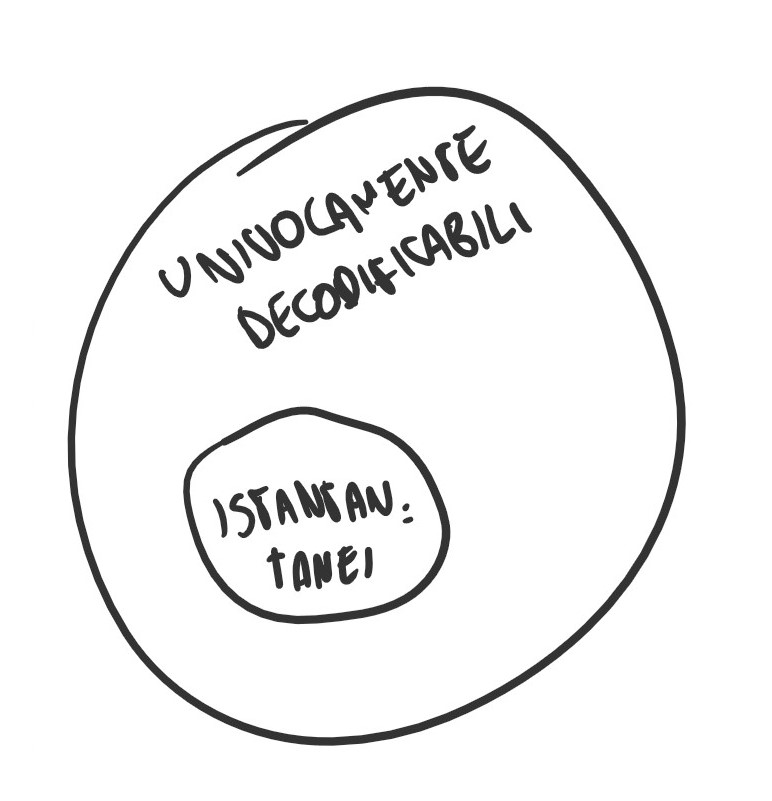
\includegraphics[width=0.5\linewidth]{immagini/img15}
	\caption{I codici istantanei sono un sottoinsieme dei codici univocamente decodificabili}
\end{figure}

\begin{center}
	\large{\textbf{Importante}\\
	$\downarrow$}
\end{center}

\tcbox[tikznode]{Non è vero che \underline{il codice è istantaneo/univocamente decodificabile se $K \leq 1$}\\ ma è vero che \textit{esiste} un codice istantaneo con quelle caratteristiche\\($r$-ario con $q$ caratteri con lunghezze $\ell_1, \ell_2, ... ,\ell_q$) se e solo se $K\leq1$}.

Riprendiamo come esempio questo codice non istantaneo:

\begin{equation*}
s_1 \rightarrow 0
\end{equation*}
\begin{equation*}
s_2 \rightarrow 01
\end{equation*}
\begin{equation*}
s_3 \rightarrow 011
\end{equation*}
\begin{equation*}
s_4 \rightarrow 111
\end{equation*}

Rigirando le cifre codificate:

\begin{equation*}
s_1 \rightarrow 0
\end{equation*}
\begin{equation*}
s_2 \rightarrow 10
\end{equation*}
\begin{equation*}
s_3 \rightarrow 110
\end{equation*}
\begin{equation*}
s_4 \rightarrow 111
\end{equation*}

Otteniamo un codice istantaneo!

Effettivamente la $K$ di Kraft accede solo alle lunghezze delle codeword ($\ell_i$) e il numero di simboli con cui scriviamo le codeword ($r$).\\
Questo per dire che le caratteristiche del codice possono renderlo istantaneo, ma sta poi a chi codifica farlo diventare istantaneo.

\subsection*{Disuguaglianza di McMillan}
\addcontentsline{toc}{subsection}{Disuguaglianza di McMillan}

\begin{theorem}
Condizione necessaria e sufficiente affinchè \textbf{esista} un codice univocamente decodificabile $r$-ario per una sorgente di $q$ simboli con codeword di lunghezze $\ell_1, \ell_2, ... , \ell_q$ è che valga:
\begin{equation}
K=\sum_{i=1}^q\frac{1}{r^{\ell_i}}\leq 1
\end{equation}
\end{theorem}

\begin{enumerate}
	\item Per ogni codice univocamente decodificabile $r$-ario per una sorgente di $q$ simboli con codeword di lunghezze $\ell_1, \ell_2,...,\ell_q$ $\rightarrow K \leq 1$.
	\item Se $K \leq 1$ allora esiste un codice univocamente decodificabile $r$-ario con lunghezze $\ell_1,\ell_2,...,\ell_q$.
\end{enumerate}

\begin{dimostrazione}
Dividiamo l'enunciato del teorema nelle due considerazioni fatte sopra.


\vspace{2mm}
\textbf{Parte 2}:\\
Se $K \leq 1 \rightarrow$ (per Kraft) esiste un codice istantaneo $r$-ario con lunghezze $\ell_1,\ell_2,...,\ell_q$.
Lo stesso codice è univocamente decodificabile (istantaei sono un sottoinsieme di univocamente decodificabili).\\


\vspace{2mm}
\textbf{Parte 1}:\\
Eleviamo $K^n$, dove $n>1$ intero. Quindi avremo che:
\begin{equation*}
K^n=[\sum_{i=1}^{q}\frac{1}{r^{\ell_i}}]^n
\end{equation*}
Definiamo $\ell=max\{\ell_1,\ell_2,...,\ell_q\}$, quindi riscriviamo la sommatoria come:
\begin{equation*}
K^n=\sum_{t=n}^{n\ell}\frac{Nt}{r^{t}}
\end{equation*}
\begin{center}
	N.B. passaggio simile a quello effettuato nella dimostazione della seconda parte di Kraft
\end{center}
Da qui noto che il numeratore $Nt$ è il numero di codeword di lunghezza $t$, ma questo numero non può essere maggiore di $r^t$ visto che rappresenta tutti i possibili vettori lunghi $t$ dove ogni elemento è un carattere dell'alfabeto $r$-ario.
\begin{equation*}
Nt \leq r^t
\end{equation*}
Quindi posso maggiorare la sommatoria:
\begin{equation*}
K^n \leq \sum_{t=n}^{n\ell}\frac{Nt}{r^{t}} = \sum_{t=n}^{n\ell}1 = n\ell-n+1= n\ell-(n-1)
\end{equation*}
$(n-1)$ è negativo visto che per ipotesi $n > 0$, quindi:
\begin{equation*}
K^n \leq n\ell
\end{equation*}
Analizziamo quindi i diversi casi:
\begin{figure}[h]
	\centering
	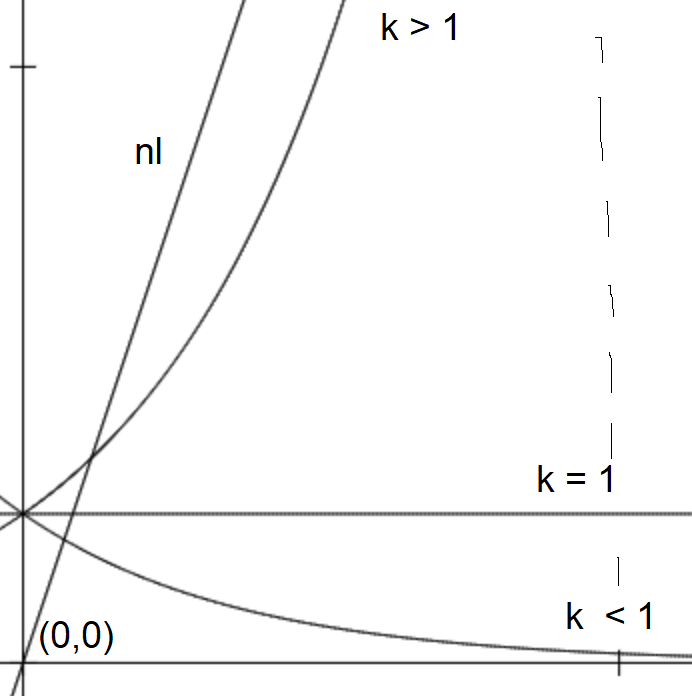
\includegraphics[width=0.5\linewidth]{immagini/img16}
\end{figure}


In maniera asintotica la disuguaglianza è rispettata solo da $k=1$ e $k<1$, quindi questo conclude la dimostazione.
\end{dimostrazione}

Una domanda che potrebbe sorgere è: ha senso utilizzare codici univocamente decodificabili ma non istantanei? No perchè lo sforzo per trovarli è uguali, quindi inutile perderere tempo su codici non istantanei.

Date le probabilità dei simboli qual è il modo più veloce per creare un codice istantaneo che minimizzi $L=\sum_{i=1}^qp_i\ell_i$?

\newpage
\subsection*{Codici a blocchi accorciati}
\addcontentsline{toc}{subsection}{Codici a blocchi accorciati}
Si parte da codeword di lunghezza uguale per poi accorciare.Facciamo un esempio:\\
$r$ = 2\\
$q=5$\\
Per rappresentare 5 simboli ci servono 3 bit; tutte le possibili combinazioni sono:
\begin{center}
	000\\001\\010\\011\\100\\101\\110\\111
\end{center}
Dobbiamo utilizzarne solo 5, quindi scartiamone 3
\begin{center}
	000 $s_1$\\$\cancel{001}$\\010 $s_2$\\$\cancel{011}$\\100 $s_3$\\$\cancel{101}$\\110 $s_4$\\111 $s_5$
\end{center}

A questo punto creiamo un albero di decodifica:

\begin{figure}[H]
	\centering
	\vspace{4mm}
	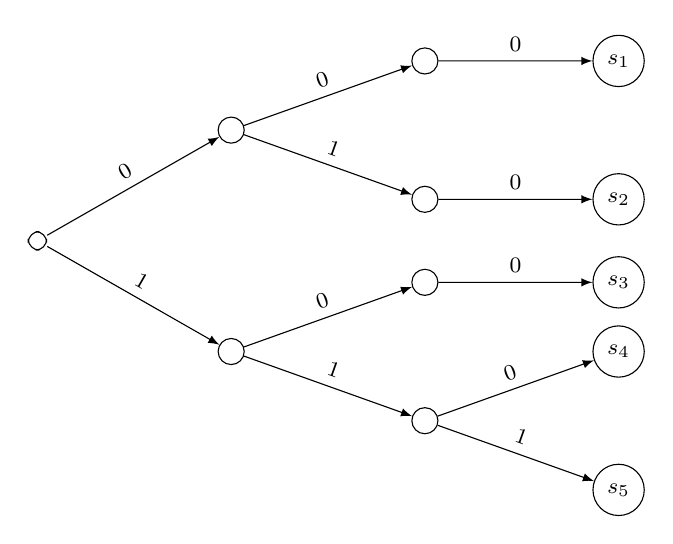
\begin{tikzpicture}
	[
	grow                    = right,
	level 1/.style={sibling distance=8em},
	level 2/.style={sibling distance=5em},
	level distance          = 7em,
	edge from parent/.style = {draw, -latex},
	every node/.style       = {font=\footnotesize},
	sloped
	]
	\node [root] {}
		child { node [dummy] {}
				child { node [dummy] {}
					child { node [dummy] {$s_5$}
						edge from parent node [above] {1}}
					child { node [dummy] {$s_4$}
						edge from parent node [above] {0}}
					edge from parent node [above] {1}}
				child { node [dummy] {}
					child { node [dummy] {$s_3$}
						edge from parent node [above] {0}}
					edge from parent node [above] {0}}
				edge from parent node [above] {1}}
		child { node [dummy] {}
			child { node [dummy] {}
				child { node [dummy] {$s_2$}
					edge from parent node [above] {0}}
			edge from parent node [above] {1}}
			child { node [dummy] {}
				child { node [dummy] {$s_1$}
					edge from parent node [above] {0}}
				edge from parent node [above] {0}}
			edge from parent node [above] {0}}
	;
	\end{tikzpicture}
	\caption{Albero di decodifica codice a blocchi}
\end{figure}

Partendo dall'albero di questo codice a blocchi, posso effettuare un processo di "sfoltimento" sui nodi di decisione con solo un figlio:

\begin{figure}[H]
	\centering
	\vspace{4mm}
	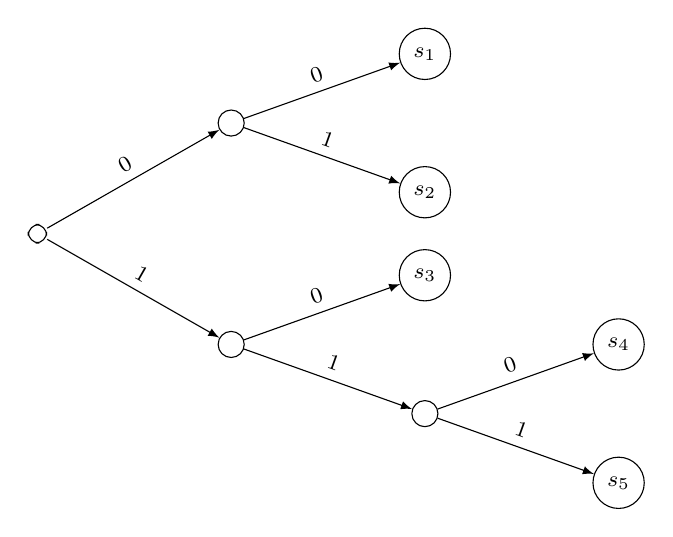
\begin{tikzpicture}
	[
	grow                    = right,
	level 1/.style={sibling distance=8em},
	level 2/.style={sibling distance=5em},
	level distance          = 7em,
	edge from parent/.style = {draw, -latex},
	every node/.style       = {font=\footnotesize},
	sloped
	]
	\node [root] {}
	child { node [dummy] {}
		child { node [dummy] {}
			child { node [dummy] {$s_5$}
				edge from parent node [above] {1}}
			child { node [dummy] {$s_4$}
				edge from parent node [above] {0}}
			edge from parent node [above] {1}}
		child { node [dummy] {$s_3$}
			edge from parent node [above] {0}}
		edge from parent node [above] {1}}
	child { node [dummy] {}
		child { node [dummy] {$s_2$}
			edge from parent node [above] {1}}
		child { node [dummy] {$s_1$}
			edge from parent node [above] {0}}
		edge from parent node [above] {0}}
	;
	\end{tikzpicture}
	\caption{Albero sfoltito a partire dal precedente}
\end{figure}

Ma come facciamo ad assicurarci che questa sia la migliore codifica per questo problema?

\subsection*{Codici di Huffman}
\addcontentsline{toc}{subsection}{Codici di Huffman}

I codici restituiti dall'algoritmo di Huffman sono \textbf{ottimali}, quindi il valore di $L=\sum_{i=1}^qp_i\ell_i$ è minimo.

Ordiniamo le probabilità dalla più grande alla più piccola (ordine non crescente):

\begin{equation*}
p_1 \geq p_2 \geq ... \geq p_q
\end{equation*}

allora un codice ottimale deve associare queste probabilità alle lunghezze poste in ordine crescente:

\begin{equation*}
\ell_1 \leq \ell_2 \leq ... \leq \ell_q
\end{equation*}

Se questo non è verificato allora il codice non è ottimale.

\begin{dimostrazione}
Assumiamo che le probabiltà siano ordinate in ordine non crescente.\\
Esistono due indici $m$ e $n$ con $m<n$ tali per cui $p_m > p_n$ e $\ell_m > \ell_n$ (quindi viola la regola di prima).
Se questo è vero, posso scambiare le codeword e ottenere una lunghezza media più piccola, quindi il codice iniziale da cui siamo partiti non era ottimale.
Il contributo nella $L$ prima dello scambio era $p_m\ell_m + p_n\ell_n$, questo contributo diventerà $p_m\ell_n+p_n\ell_m$.
La differenza fra queste quantità vale
\begin{equation*}
p_m\ell_n+p_n\ell_m-p_m\ell_m+p_n\ell_n
\end{equation*}
\begin{equation*}
= p_m(\ell_n-\ell_m)-p_n(\ell_n-\ell_m)
\end{equation*}
\begin{equation*}
= (p_m-p_n)(\ell_n-\ell_m)
\end{equation*}
Queste due quantità sono rispettivamente $>0$ e $<0$, quindi la differenza è negativa, quindi scambiando le codeword avrò una lunghezza media minore.
Quindi questo dimostra che sono partito da un codice non ottimale in quanto le lunghezze delle codeword non sono in ordine non decrescente.
\end{dimostrazione}

Ora riconsideriamo

\begin{equation*}
p_1 \geq p_2 \geq ... \geq p_{q-1} \geq p_q
\end{equation*}
\begin{equation*}
\ell_1 \leq \ell_2 \leq ... \leq \ell_{q-1} \leq \ell_q
\end{equation*}

I due simboli meno probabili avranno codeword di uguale lunghezza, per costruzione dell'albero (si apre sempre in due, quindi $\downarrow$)

\begin{figure}[h]
	\centering
	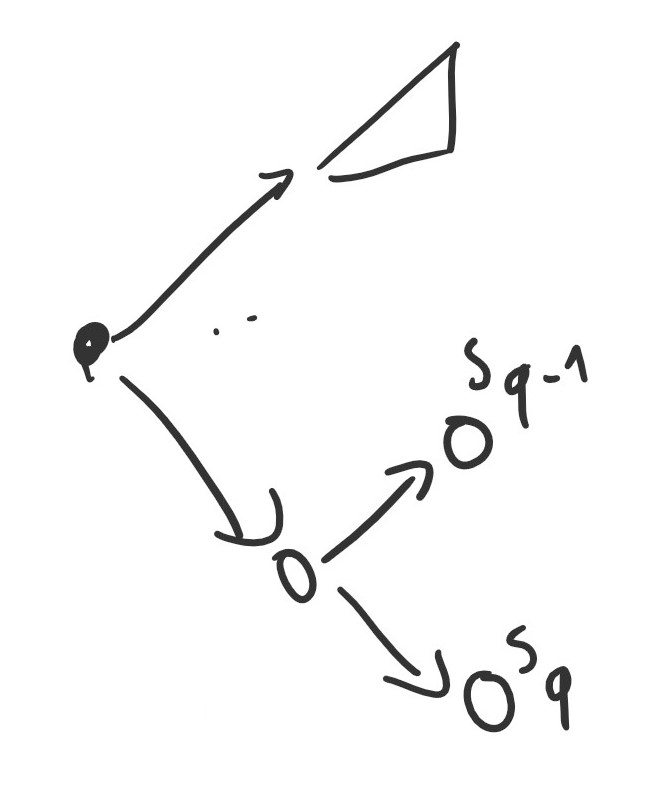
\includegraphics[width=0.3\linewidth]{immagini/img17}
\end{figure}

Quindi per concludere: se le probabilità e le lunghezze seguono la regola precedente e questa regola appena spiegata è rispettata, allora il codice è ottimale.
Ma come creo un codice ottimale?
\newpage
Facciamo un esempio di esecuzione di Algoritmo di Huffman.\\
$r=2$, Abbiamo cinque simboli che escono con le seguenti probabilità:
\begin{center}
	$p_1 = 0.4$\\
	$p_2 = 0.2$\\
	$p_3 = 0.2$\\
	$p_4 = 0.1$\\
	$p_5 = 0.1$
\end{center}
L'algoritmo di Huffman ha un esecuzione di tipo greedy e funziona così:
\begin{enumerate}
\item Prendo i due simboli meno probabili e creo un simbolo 'virtuale' combinandoli, quindi dall'esempio prima otterrò:
\begin{center}
	$p_1 = 0.4$\\
	$p_2 = 0.2$\\
	$p_3 = 0.2$\\
	\hspace{20mm}$p_{4,5} = 0.1 + 0.1=0.2$
\end{center}
\item Itero il passaggio precedente mantenendo traccia delle varie unioni:
\begin{multicols}{3}
	\begin{center}
		$p_1 = 0.4$\\
		$p_2 = 0.2$\\
		$p_3 = 0.2$\\
		$p_{4,5} = 0.2$
	\end{center}
	
	\columnbreak
	
	\begin{center}
		$p_1 = 0.4$\\
		$p_{3,4,5} = 0.4$\\
		$p_2 = 0.2$
	\end{center}  

	\columnbreak
	
	\begin{center}
		$p_1 = 0.4$\\
		$p_{2,3,4,5} = 0.6$
	\end{center}
\end{multicols}
\item Mi fermo quando ottengo $r$ probabilità e assegno un carattere ciascuno:
\begin{center}
	$p_1 = 0.4 \rightarrow \texttt{0}$\\
	$p_{2,3,4,5} = 0.6 \rightarrow \texttt{1}$
\end{center}
\item Ora itero all'indietro, appendendo un carattere alla volta nelle probabilità virtuali (appendo alla fine, se no creo prefissi e il codice non è più istantaneo), quando una virtuale ha lunghezza uguale a un altro simbolo la metto sotto.
\small{
\begin{multicols}{4}
	\begin{center}
		$p_{2,3,4,5} = 0.6 \rightarrow \texttt{0}$
		$p_1 = 0.4 \rightarrow \texttt{1}$\\
	\end{center}
	
	\columnbreak
	
	\begin{center}
		$p_1 = 0.4 \rightarrow \texttt{1}$\\
		$p_{3,4,5} = 0.4 \rightarrow \texttt{00}$
		$p_{2} = 0.2 \rightarrow \texttt{01}$
	\end{center}  
	
	\columnbreak
	
	\begin{center}
		$p_1 = 0.4 \rightarrow \texttt{1}$\\
		$p_{2} = 0.2 \rightarrow \texttt{01}$
		$p_{3} = 0.2 \rightarrow \texttt{000}$
		$p_{4,5} = 0.2 \rightarrow \texttt{001}$
	\end{center}

\columnbreak

\begin{center}
	$p_1 = 0.4 \rightarrow \texttt{1}$\\
	$p_{2} = 0.2 \rightarrow \texttt{01}$
	$p_{3} = 0.2 \rightarrow \texttt{000}$
	$p_{4} = 0.1 \rightarrow \texttt{0010}$
	$p_{5} = 0.1 \rightarrow \texttt{0011}$
\end{center}

\end{multicols}
}
\footnotesize{
Si noti come la regola delle probabilità in ordine inverso rispetto alle lunghezze sia rispettata in tutti i passaggi.
}

\end{enumerate}
Quanto vale la lunghezza media del codice appena calcolato?
\begin{equation*}
L = \sum_{i=1}^qp_i\ell_i = 0.4 \cdot 1 + 0.2 (2+3) + 0.1 \cdot (4+4) = 
\end{equation*}
\begin{equation*}
= 0.4 + 0.2 \cdot 5 + 0.1 \cdot 8 = 0.4 +1+0.8 = 2.2\frac{bit}{simbolo}
\end{equation*}

Proviamo a effettuare un altra esecuzione variando una regola, nel caso due simboli abbiano stessa probabilità, metto sopra quello virtuale (prima era il contrario):
\small{
	\begin{multicols}{4}
		\begin{center}
			$p_1 = 0.4 \rightarrow \texttt{00}$\\
			$p_{2} = 0.2 \rightarrow \texttt{10}$
			$p_{3} = 0.2 \rightarrow \texttt{11}$
			$p_{4} = 0.1 \rightarrow \texttt{010}$
			$p_{5} = 0.1 \rightarrow \texttt{011}$
		\end{center}
		
		\begin{center}
			$p_1 = 0.4 \rightarrow \texttt{00}$\\
			$p_{4,5} = 0.2 \rightarrow \texttt{01}$\\
			$p_{2} = 0.2 \rightarrow \texttt{10}$\\
			$p_{3} = 0.2 \rightarrow \texttt{11}$	
		\end{center}
	
		
		\columnbreak
		
		\begin{center}
			$p_{2,3} = 0.4 \rightarrow \texttt{1}$
			$p_1 = 0.4 \rightarrow \texttt{00}$\\
			$p_{4,5} = 0.2 \rightarrow \texttt{01}$
		\end{center}  
	
		\columnbreak
		
		\begin{center}
			$p_{1,4,5} = 0.6 \rightarrow \texttt{0}$
			$p_{2,3} = 0.4 \rightarrow \texttt{1}$\\
		\end{center}
		
		\columnbreak
	\end{multicols}
}
\normalsize

Le codeword ottenute sono ovviamente diverse, ma la lunghezza media rimarrà uguale:

\begin{equation*}
L = \sum_{i=1}^qp_i\ell_i = 0.4 \cdot 2 + 0.2 (2+2) + 0.1 \cdot (3+3) = 
\end{equation*}
\begin{equation*}
= 0.8 + 0.2 \cdot 4 + 0.1 \cdot 6 = 0.8 +0.8+0.6 = 2.2\frac{bit}{simbolo}
\end{equation*}

Quello che cambia sarà la varianza.






\newpage
\section*{Lezione 8}
\addcontentsline{toc}{section}{Lezione 8}



\newpage
\section*{Lezione 9}
\addcontentsline{toc}{section}{Lezione 9}

\subsection*{Teoria dell'informazione - Entropia}
\addcontentsline{toc}{subsection}{Teoria dell'informazione - Entropia}

Prendiamo una sorgente $S = {s_1, s_2, ..., s_q}$ caratterizzato dalle probabilità $p_1, p_2, ... , p_q$.
Definiamo una funzione $I(s_i) / I(p_i)$ come la quantità di informazione data da un simbolo.
La quantità di informazione è proporzionale alla "sorpresa" che abbiamo nel leggere il simbolo.

Dominio:
\begin{equation*}
I:S\rightarrow {\rm I\!R}
\end{equation*} 

Inversamente proporzionale alla probabilità:
\begin{equation*}
I(p_i) = \frac{1}{p_i}
\end{equation*}

Abbiamo bisogno inoltre della proprietà additiva: l'informazione di due eventi stocastici indipendenti si sommano:
\begin{equation*}
I(p_i) + I(p_j) = \frac{1}{p_i} + \frac{1}{p_j} = \frac{p_j+p_i}{p_ip_j}
\end{equation*}

Ma quello che accade nella realtà è che la probabilità che avvengano due eventi è

\begin{equation*}
I(p_ip_j) = \frac{1}{p_ip_j}
\end{equation*}

Quindi la funzione $I=\frac{1}{p_i}$ non gode della proprietà additiva, quindi la scartiamo.

Cerchiamo di capire come si comporta la funzione che stiamo cercando:
\begin{enumerate}
	\item $I(p) \geq 0 \; \; \; \; \; (positivita)$
	\item $I(p_1p_2) = I(p_1) + I(p_2) \; \; \; \; \; (additivita)$\\
	se gli eventi sono indipendenti
	\item $I \; \text{è una funzione continua di p}$
\end{enumerate}

Notiamo che $I(p^n) = nI(p)$

\textbf{Base induzione:}\\
$I(p) = I(p)$\\
\textbf{Passo induttivo:}\\
Supponiamo che valga $I(p^{n-1}) = (n-1)I(p)$,\\
$I(p^n) = I(pp^{n-1}) = I(p) + I(p^{n-1}) = I(p) + (n-1)I(p) = nI(p)$

\newpage
Ora definiamo $y=p^n$, da cui ricaviamo che $p=y^{\frac{1}{n}}$.
Poi calcoliamo $I(y)=I(p^n)=nI(p)=nI(y^{\frac{1}{n}})$.
\begin{equation*}
I(y^{\frac{1}{n}}) = \frac{1}{n}I(Y) \; \; \; \; \; \; \forall n \in N
\end{equation*}
Ora estendiamo per tutti i numeri razionali:

\begin{equation*}
I(y^{\frac{m}{n}}) = I((y^{\frac{1}{n}})^m) = mI(y^{\frac{1}{n}}) = \frac{m}{n}I(y)
\end{equation*}

Osserviamo queste proprietà, c'è una funzione che le rispetta tutte: il logaritmo.

\begin{equation*}
I(p) = k\cdot \log p
\end{equation*}
per $k=-1$ ottengo:

\begin{empheq}[box=\tcbhighmath]{equation*}
I(p) = \log \frac{1}{p}
\end{empheq}

La proprietà di additività è rispettata:
\begin{equation*}
I(p_1) + I(p_2) = \log \frac{1}{p_1} + \log \frac{1}{p_2} = \log \frac{1}{p_1p_2} = I(p_1p_2)
\end{equation*}

Quale base utilizziamo per il logaritmo? Essa ci fornisce l'unità di misura con cui calcoliamo la quantità di informazione.
La base più utilizzata in natura è $e$, mentre nel mondo digitale si utilizza molto la base 2.


Quanto si calcola in $ln$ l'unità di misura dell'informazione è \textit{nat}, in base 2 l'unità di misura è il \textit{bit}, in base 10 si misura in \textit{Hartley}. In ogni caso posso cambiare base velocemente moltiplicando per una costante $C$.



Ma il logaritmo è l'unica funzione che va bene per rappresentare la funzione $I$?

\begin{dimostrazione}
Fissiamo $I(p)=\log_2\frac{1}{p}$.\\
Abbiamo già visto questa proprietà:
\begin{equation*}
I(p^n)=nI(p)
\end{equation*}
Supponiamo che esista una funzione $g$ per cui $g(p^n)=ng(p)$ che sia continua, e che restituisca valori $\geq 0$.

Proviamo a calcolare la differenza fra il logaritmo e questa ipotetica funzione:

\begin{equation*}
g(p^n) - C \log_2\frac{1}{p^n} = n[g(p)-C\log_2 \frac{1}{p}]
\end{equation*}
Poniamo $C=\frac{g(p_0)}{\log_2\frac{1}{p_0}}$, con $p_0 \neq 0, 1$, quindi diverso dagli estremi. In questo modo la differenza fra le due diventa zero.
\newpage
Ora possono succedere due cose:
\begin{itemize}
	\item Due funzioni completamente diverse:
	\begin{figure}[H]
		\centering
		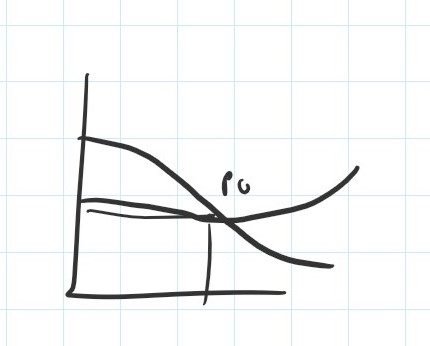
\includegraphics[width=0.3\linewidth]{immagini/img23}
	\end{figure}
		
	\item Due funzioni che sembrano diverse ma sono la stessa funzione:
	\begin{figure}[H]
		\centering
		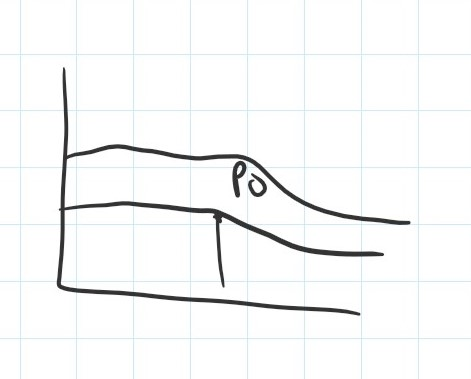
\includegraphics[width=0.3\linewidth]{immagini/img24}
	\end{figure}
\end{itemize}

Sfrutto una proprietà dall'analisi matematica per cui ogni numero reale può essere scritto come:

\begin{equation*}
\forall \; z \; \exists \; n \; \; | \; \; z=p_0^n
\end{equation*}

Quindi per $p=p_0$ posso scrivere:

\begin{equation*}
g(z) - C \; log_2\frac{1}{z} = 0
\end{equation*}
Uguale a 0 in quanto $C=\frac{g(p_0)}{\log_2\frac{1}{p_0}}$ annulla l'equazione sopra
\begin{equation*}
g(z) = C \; log_2\frac{1}{z}
\end{equation*}
Quindi questa funzione si dimostra essere un logaritmo
\end{dimostrazione}  

Quindi abbiamo definito l'unica funzione possibile per definire la quantità di informazione per un evento.


Consideriamo una sorgente $S$ che emette $q$ simboli con $p_1, p_2, ..., p_q$.
Abbiamo quindi detto che:
\begin{equation*}
I(s_i)=I(p_i)=log_r\frac{1}{p_i}
\end{equation*}

Quanto è la quantità di informazione media data una sorgente? Chiamo questo valore come $H(s)$.
Per calcolare questo valore peso ogni quantità di informazione:

\begin{equation*}
H(s) = p_1I(s_1) + p_2I(s_2) + ... + p_qI(s_q)
\end{equation*}

Riscriviamo in forma compatta:

\begin{equation*}
H(s) = \sum_{i=1}^qp_iI(s_i)
\end{equation*}

\begin{equation*}
H(s) = \sum_{i=1}^qp_i\log\frac{1}{p_i}
\end{equation*}
oppure scritto come
\begin{equation*}
H(s) = -\sum_{i=1}^qp_i\log{p_i}
\end{equation*}

Questa formula appena scritta è l'\textbf{entropia} di una sorgente ed è definita come:

\begin{empheq}[box=\tcbhighmath]{equation*}
H_r(s) = \sum_{i=1}^qp_i\log_r\frac{1}{p_i}
\end{empheq}

L'unità di misura dell'entropia è data dalla base del logaritmo,
\begin{equation*}
H_r(s) = H_2(s)\log_r2
\end{equation*}
Ma posso cambiare velocemente base tramite una costante.

Se una sorgente fa uscire messaggi lunghi $N$ con simboli $s_q$, mi aspetterò di avere
\begin{itemize}
	\item $N \cdot p_1$ occorrenze di $s_1$
	\item $N \cdot p_2$ occorrenze di $s_2$
	\item ..
	\item $N \cdot p_q$ occorrenze di $s_q$
\end{itemize}

La probabilità $P$ di avere un messaggio fatto in questo modo sarà:
\begin{equation*}
P = p_1^{Np_1} \cdot p_2^{Np_2} \cdot ... \cdot p_q^{Np_q} = [p_1^{p_1}p_2^{p_2}...p_q^{p_q}]^N
\end{equation*}

\newpage 

Quando esce questo messaggio, la quantità di informazione che otteniamo è $\log\frac{1}{p}$, che è quindi:

\begin{equation*}
\log\frac{1}{p} = \log\frac{1}{[p_1^{p_1}p_2^{p_2}...p_q^{p_q}]^N} = \log[\frac{1}{p_1^{p_1}p_2^{p_2}...p_q^{p_q}}]^N = N\log[\frac{1}{p_1^{p_1}} \cdot \frac{1}{p_2^{p_2}} \cdot ... \cdot \frac{1}{p_q^{p_q}}]
\end{equation*}


\begin{equation*}
= N \sum_{i=1}^q\log[\frac{1}{p_i}]^{p_i} = N \sum_{i=1}^qp_i\log\frac{1}{p_i}
\end{equation*}

Quindi l'entropia possiamo vederla come la quantità di informazione mediamente emessa dalla sorgente:

\begin{equation*}
H(s) = \frac{\log\frac{1}{p}}{N}
\end{equation*}

Vediamo ora come è fatta questa funzione entropia:

\begin{figure}[h]
	\centering
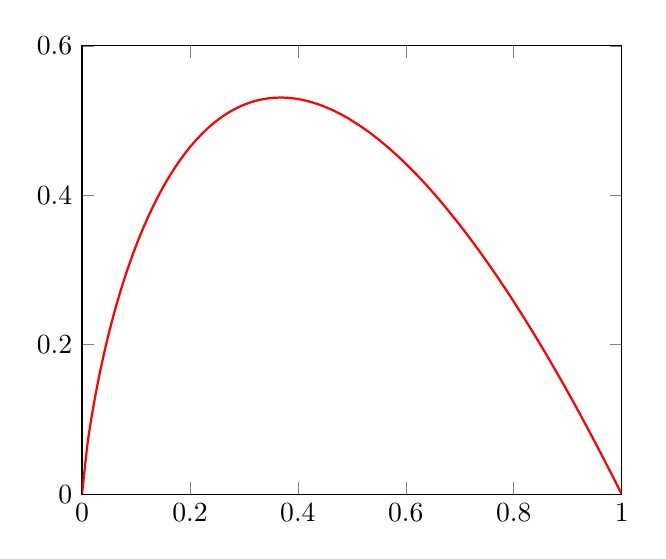
\begin{tikzpicture}
\begin{axis}[
xmin = 0, xmax = 1,
ymin = 0, ymax = 0.6,
]
\addplot[
domain = 0:1,
samples = 100,
smooth,
thick,
red,
] {x*log2(1/x)};
\end{axis}
\end{tikzpicture}
\caption{Grafico funzione $H_2(s)$}
\end{figure}

In $p=0$ abbiamo un punto di discontinuità a cui ci si avvicina con pendenza infinita, quindi definiamo formalmente un'altra funzione per cui se $p=0$ allora la funzione vale 0 (un evento impossibile non ci da informazione).

Il punto massimo vale $\frac{1}{e}$.

L'entropia $H(s)$ è sempre un valore $\geq 0$.\\
Quando vale 0? Essendo una somma di termini $\geq 0$, allora essa si annulla solo se tutti i termini sono uguali a 0, che è il caso in cui la sorgente ha come probabilità $p_1 = 1, p_2 = 0, p_3 = 0, ... p_q = 0$, quindi quando esce sempre lo stesso simbolo.


\newpage
\section*{Lezione 10}
\addcontentsline{toc}{section}{Lezione 10}

\subsection*{Sorgente Bernoulliana}
\addcontentsline{toc}{subsection}{Sorgente Bernoulliana}

Data una sorgente $S=\{s_1, s_2\}$ in cui $s_1$ ha probabilità $p$ e $s_2$ ha probabilità $1-p$, la sua entropia vale

\begin{equation*}
H_2(p) = p\log_2\frac{1}{p} + (1-p)log_2\frac{1}{1-p}
\end{equation*}

Questa è una funzione a una variabile (e non due). In generale $H_r(p_1, p_2, ..., p_q)$ è una funzione a $q-1$ variabili.
Proviamo a disegnare la funzione entropia della sorgente Bernoulliana:


\begin{figure}[h]
	\centering
	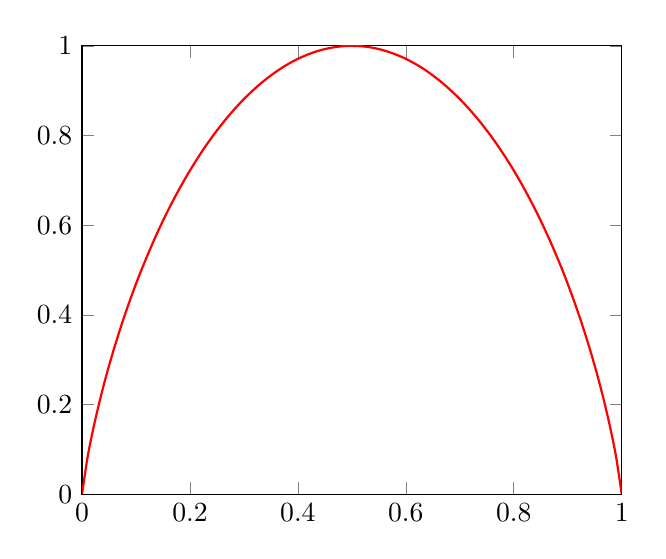
\begin{tikzpicture}
	\begin{axis}[
	xmin = 0, xmax = 1,
	ymin = 0, ymax = 1,
	]
	\addplot[
	domain = 0:1,
	samples = 100,
	smooth,
	thick,
	red,
	] {x*log2(1/x) + (1-x)*log2(1/(1-x))};
	\end{axis}
	\end{tikzpicture}
	\caption{Grafico sorgente Bernoulliana}
\end{figure}

Sembra una parabola ma non lo è (in 0 la derivata ha pendenza infinita).
Il valore massimo (1) si ottiene per $p=\frac{1}{2}$, il minimo (0) quando $p=0 \lor p=1$.
Dove si trova invece il valore massimo per il caso generale $H_r(p_1, p_2, ..., p_q)$?

\newpage

\subsection*{Disuguaglianza di Gibbs}
\addcontentsline{toc}{subsection}{Disuguaglianza di Gibbs}

\begin{figure}[h]
	\centering
	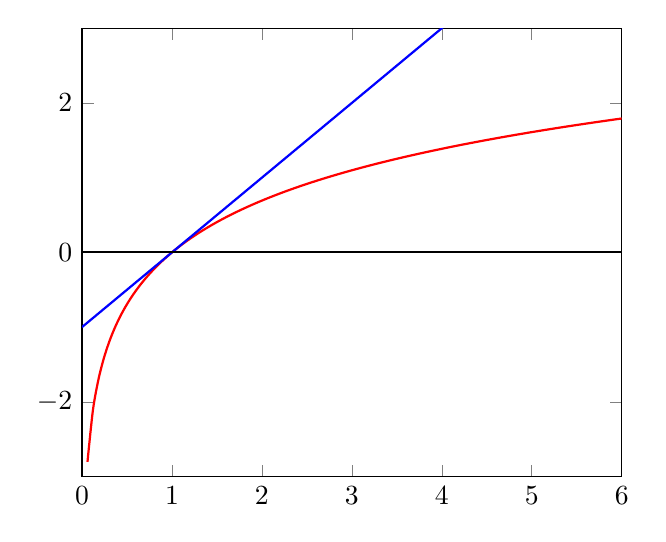
\begin{tikzpicture}
	\begin{axis}[
	xmin = 0, xmax = 6,
	ymin = -3, ymax = 3,
	]
	\addplot[
	domain = 0:6,
	samples = 100,
	smooth,
	thick,
	red,
	] {ln(x)};
		\addplot[
	domain = 0:6,
	samples = 100,
	smooth,
	thick,
	blue,
	] {x-1};
	] {ln(x)};
	\addplot[
	domain = 0:6,
	samples = 2,
	smooth,
	thick,
	black,
	] {0};
	\end{axis}
	\end{tikzpicture}
	\caption{Grafico $y=x-1$ (in blu) e $y=ln(x)$ (in rosso)}
\end{figure}

Notiamo che $ln(x) <= x - 1 \; \; \forall x > 0$ e vale $ln(x) = x$ se $x = 1$.

Prendiamo due distribuzioni di probabilità
\begin{equation*}
x_1, x_2, ... , x_q
\end{equation*}
\begin{equation*}
y_1, y_2, ... , y_q
\end{equation*}
La disuguaglianza di Gibbs ci dice che:
\begin{empheq}[box=\tcbhighmath]{equation*}
\sum_{i=1}^qx_i\log_2(\frac{y_i}{x_i}) \leq 0
\end{empheq}

\textbf{Dimostrazione non richiesta all'orale}, però la scrivo dai

\begin{dimostrazione}
	Partiamo da:
	\begin{equation*}
	\sum_{i=1}^qx_i\log_2(\frac{y_i}{x_i}) = \frac{1}{\ln2}\sum_{i=1}^qx_i\ln(\frac{y_i}{x_i})
	\end{equation*}
	Ora sfruttiamo la maggiorazione di prima:
	\begin{equation*}
    \frac{1}{\ln2}\sum_{i=1}^qx_i\ln(\frac{y_i}{x_i}) \leq \frac{1}{\ln2}\sum_{i=1}^qx_i(\frac{y_i}{x_i} - 1)
	\end{equation*}
		\begin{equation*}
	\frac{1}{\ln2}\sum_{i=1}^qx_i\ln(\frac{y_i}{x_i}) \leq \frac{1}{\ln2}\sum_{i=1}^q(y_i-x_i)
	\end{equation*}
		\begin{equation*}
	\frac{1}{\ln2}\sum_{i=1}^qx_i\ln(\frac{y_i}{x_i}) \leq \frac{1}{\ln2}[\sum_{i=1}^qy_i-\sum_{i=1}^qx_i]
	\end{equation*}
	Ma essendo le due sommatorie $\sum_{i=1}^qy_i-\sum_{i=1}^qx_i$ e $\sum_{i=1}^qy_i-\sum_{i=1}^qx_i$ sono uguali a 1, allora:
			\begin{equation*}
	\frac{1}{\ln2}\sum_{i=1}^qx_i\ln(\frac{y_i}{x_i}) \leq \frac{1}{\ln2}[0-0]
	\end{equation*}
	\begin{equation*}
	\sum_{i=1}^qx_i\ln(\frac{y_i}{x_i}) \leq 0
	\end{equation*}
	Questo funziona solo se $x_i = y_i$ per tutte le $i$, quindi se e solo se le due distribuzioni di probabilità sono uguali.
\end{dimostrazione}

Ora possiamo usare la disuguaglianza per trovare il valore massimo dell'entropia.

Calcoliamo

\begin{equation*}
H_2(S)-\log_2q = \sum_{i=1}^qp_ilog_2\frac{1}{p_i} - (log_2q)\sum_{i=1}^qp_i
\end{equation*}
\begin{equation*}
= \sum_{i=1}^qp_i[\log_2\frac{1}{p_i} - \log_2q] = \sum_{i=1}^qp_i\log_2\frac{1}{p_iq} = \sum_{i=1}^qp_i\log_2\frac{\frac{1}{q}}{p_i}
\end{equation*}
Applico Gibbs e scopro che:
\begin{equation*}
 \sum_{i=1}^qp_i\log_2\frac{\frac{1}{q}}{p_i} \leq 0
\end{equation*}
E quindi:
\begin{equation*}
H_2(S) \leq \log_2q
\end{equation*}
e l'entropia raggiunge il valore massimo (quindi $\log_2q$) solo quando i valori di probabilità sono uguali, quindi quando la distribuzione è uniforme.

Quindi l'entropia $H_2(S)$:
\begin{itemize}
	\item \'E sempre maggiore o uguale di zero, in particolare è $=0$ quando la distribuzione di probabilità assegna ad una $p_i$ valore 1 e al resto valore 0
	\item \' E sempre minore o uguale a $\log_2q$, e raggiunge questo valore massimo quando la distribuzione di probabilità è uniforme.
\end{itemize}

Ora supponiamo di avere una sorgente $S=\{s_1, s_2, ..., s_q\}$ che codifica un codice istantaneo $r$-ario con codeword di lunghezza $\ell_1, \ell_2, ..., \ell_q$.
Proviamo a mettere in relazione la lunghezza media con l'entropia della sorgente.
Essendo il codice istantaneo vale la disuguaglianza di Kraft:
\begin{equation*}
\sum_{i=1}^q\frac{1}{r^{\ell_i}} \leq 1
\end{equation*}

Ora definiamo per $i=1,2,...q$ 
\begin{equation*}
Q_i = \frac{r^{-\ell_i}}{K}
\end{equation*}

che sarebbe uno dei termini della somma fratto la somma totale

\begin{equation*}
0 \leq Q_i = \frac{r^{-\ell_i}}{K} \leq 1
\end{equation*}

Posso dire che

\begin{equation*}
\{Q_1, Q_2, ..., Q_q\}
\end{equation*}
è una distribuzione di probabilità, e vale $\sum_{i=1}^qQ_i = 1$.
(P.S. questo conto qua non serve orale)

Ora uso queste due distribuzioni per scrivere la disuguaglianza di Gibbs

\begin{equation*}
\sum_{i=0}^qp_i\log_2\frac{Q_i}{p_i} \leq 0
\end{equation*}

Ora lavoriamoci su:

\begin{equation*}
\sum_{i=0}^qp_i\log_2\frac{Q_i}{p_i} =
\end{equation*}
\begin{equation*}
= \highlight{\sum_{i=0}^qp_i[\log_2\frac{1}{p_i}} - \log_2\frac{1}{Q_i}]
\end{equation*}
\begin{equation*}
= H_2(S) - \sum_{i=0}^qp_i\log_2\frac{1}{Q_i} \leq 0
\end{equation*}
\begin{equation*}
= H_2(S) \leq \sum_{i=0}^qp_i\log_2\frac{1}{Q_i}
\end{equation*}
\begin{equation*}
= H_2(S) \leq \sum_{i=0}^qp_i\log_2\frac{K}{r^{-\ell_i}}
\end{equation*}
\begin{equation*}
= H_2(S) \leq \sum_{i=0}^qp_i[\log_2K - \log_2{r^{-\ell_i}}]
\end{equation*}
\begin{equation*}
= H_2(S) \leq \log_2K \sum_{i=0}^qp_i + \log_2{r^{-\ell_i}}
\end{equation*}
\begin{equation*}
= H_2(S) \leq \log_2K \sum_{i=0}^qp_i + \log_2r\sum_{i=1}^qp_i\ell_i
\end{equation*}
\begin{equation*}
= H_2(S) \leq \log_2K + \log_2r \cdot L
\end{equation*}

Noto che $K \leq 1$, quindi il logaritmo di un valore minore di 1 è $\leq 0$, quindi posso minorare ulteriormente

\begin{equation*}
= H_2(S) \leq \log_2r \cdot L
\end{equation*}

Riscrivo tutto come:

\begin{equation*}
\frac{1}{\log_2r} \cdot H_2(S) \leq L
\end{equation*}
La quantità $\frac{1}{\log_2r}$ fa un cambio di base nel logaritmo dell'entropia, quindi:

\begin{empheq}[box=\tcbhighmath]{equation*}
H_r(S) \leq L
\end{empheq}

Questa disuguaglianza mi dice che data una sorgente $S$ istantanea con una lunghezza media $L$, essa non può essere più piccola dell'entropia misurata in base $r$.
Quindi la lunghezza media non può essere più piccola dell'entropia.\\
Quando rappresento in maniera compatta è come se le stessi comprimendo delle sequenze, se scendo sotto una certa soglia vuol dire che sto perdendo informazione. Quindi l'entropia rappresenta anche una soglia minima per quanto riguarda la lunghezza media delle codeword.\\
In pratica più mi avvicino all'entropia più sto comprimendo la lunghezza media.

\medskip
La seguente disuguaglianza vale anche per i codici univocamente decodificabili (thanks McMillan) visto che la regola sulla $K$ vale anche su di essi.

\medskip

Quando però questa disuguaglianza diventa una uguaglianza (quindi ottengo la compressione massima)?

Nel passaggio da:

\begin{equation*}
= H_2(S) \leq \log_2K + \log_2r \cdot L
\end{equation*}

a

\begin{equation*}
= H_2(S) \leq \log_2r \cdot L
\end{equation*}

Dobbiamo fare in modo che $\log_2K$ sia uguale a 0, ovvero quando $K=1$. 

\subsection*{Codifica di Shannon-Fano}
\addcontentsline{toc}{subsection}{Codifica di Shannon-Fano}

Shannon e Fano partono da:

\begin{equation*}
H_r(S) \leq  L
\end{equation*}

che è un confronto fra medie (somma pesata vs somma pesata), ma vale la stessa cosa anche singolarmente?

\begin{equation*}
log_r\frac{1}{p_i} \leq \ell_i
\end{equation*}

Se fosse vero allora posso conoscere la lunghezza di una codeword a partire da $p_i$. Possiamo anche dire che $\ell_i$ è l'unico intero compreso in questo intervallo:

\begin{equation*}
log_r\frac{1}{p_i} \leq \ell_i < log_r\frac{1}{p_i} + 1
\end{equation*}

Chiamo queste lunghezze $\ell_i$ \textit{lunghezze di Shannon-Fano}.
Ma che tipo di codici ottengo con queste lunghezze? Codici istantanei; per dimostrarlo parto dalla disuguaglianza sopra (orale chiede):

\begin{equation*}
log_r\frac{1}{p_i} \leq \ell_i < log_r\frac{1}{p_i} + 1
\end{equation*}
\begin{equation*}
r^{log_r\frac{1}{p_i}} \leq r^{\ell_i} < r^{log_r\frac{1}{p_i} + 1}
\end{equation*}
\begin{equation*}
\frac{1}{p_i} \leq r^{\ell_i} < \frac{r}{p_i}
\end{equation*}
\begin{equation*}
p_i \geq \frac{1}{r^{\ell_i}} > \frac{p_i}{r}
\end{equation*}

Ora sommo tutte le $i$:
\begin{equation*}
\sum_{i=0}^qp_i \geq \sum_{i=0}^q\frac{1}{r^{\ell_i}} > \sum_{i=0}^qp_i\frac{1}{r}
\end{equation*}
\begin{equation*}
1\geq K > \frac{1}{r}
\end{equation*}

Quindi con queste lunghezze vale Kraft, quindi sono in grado di costruire un codice istantaneo.
La codifica di Shannon-Fano ci dice date le probabilità come sono definite le lunghezze, ma come trovo poi le codeword? Con l'albero di decodifica.

Ma allora perchè studiare Huffman? Esso ritorna un codice ottimale, vale anche per Shannon-Fano?

Siamo sicuri che 

\begin{equation*}
L_{\text{Huffman}} \leq L_{\text{Shannon-Fano}}
\end{equation*}

Andiamo a calcolare la lunghezza media di un codice creato tramite Shannon-Fano:

\begin{equation*}
log_r\frac{1}{p_i} \leq \ell_i < log_r\frac{1}{p_i} + 1
\end{equation*}
\begin{equation*}
p_i\log_r\frac{1}{p_i} \leq p_i\ell_i < p_i\log_r\frac{1}{p_i} + p_i
\end{equation*}
\begin{equation*}
\sum_{i=0}^qp_i\log_r\frac{1}{p_i} \leq \sum_{i=0}^qp_i\ell_i < \sum_{i=0}^qp_i\log_r\frac{1}{p_i} + \sum_{i=0}^qp_i
\end{equation*}
\begin{equation*}
H_r(S) \leq L_{Shannon-Fano} \leq H_r(S) + 1
\end{equation*}
E questo lo abbiamo già visto prima, però ci dice anche che non saranno mai più grandi di 1 dall'ottimo.
In pratica magari non saranno sempre ottimali, però nel caso non lo fossero non sono così tanto peggiori dell'ottimale.
In conclusione Huffman è più lento ma ottimale, Shannon Fano più veloce ma non sempre ottimale (ma non così male).

Vediamo un esempio di applicazione della codifica.

Sorgente con 6 simboli: $p_1 = p_2 = \frac{1}{4}$ $p_3 = p_4 = p_5 = p_6 = \frac{1}{8}$ con $r=2$.
Dobbiamo trovare il più piccolo $\ell_1$ tale per cui $log_2\frac{1}{p_i} \leq \ell_i$.

\begin{equation*}
\log_2\frac{1}{\frac{1}{4}} \leq \ell_1
\end{equation*}
\begin{equation*}
\log_24 \leq \ell_1
\end{equation*}
\begin{equation*}
2 \leq \ell_1
\end{equation*}
\begin{equation*}
\ell_1 = 2
\end{equation*}
\begin{equation*}
\ell_2 = 2
\end{equation*}

Quindi ho trovato le prime due.

\begin{equation*}
\log_2\frac{1}{\frac{1}{8}} \leq \ell_3
\end{equation*}
\begin{equation*}
\log_28 \leq \ell_3
\end{equation*}
\begin{equation*}
\ell_3 = 3
\end{equation*}
\begin{equation*}
\ell_4 = 3
\end{equation*}
\begin{equation*}
\ell_5 = 3
\end{equation*}
\begin{equation*}
\ell_6 = 3
\end{equation*}

Quindi costruisco l'albero a partire dalle lunghezze trovate:

\begin{figure}[H]
	\centering
	\vspace{4mm}
	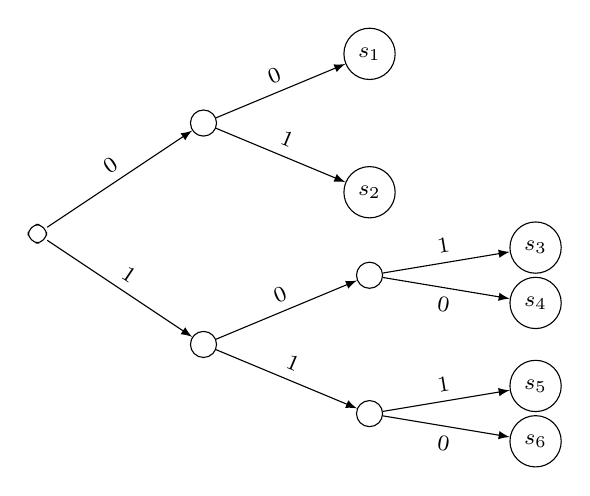
\begin{tikzpicture}
	[
	grow                    = right,
	level 1/.style={sibling distance=8em},
	level 2/.style={sibling distance=5em},
	level 3/.style={sibling distance=2em},
	level distance          = 6em,
	edge from parent/.style = {draw, -latex},
	every node/.style       = {font=\footnotesize},
	sloped
	]
	\node [root] {}
	child { node [dummy] {}
		child { node [dummy] {}
			child { node [dummy] {$s_6$}
				edge from parent node [below] {0}}
			child { node [dummy] {$s_5$}
				edge from parent node [above] {1}}
			edge from parent node [above] {1}}
		child { node [dummy] {}
			child { node [dummy] {$s_4$}
				edge from parent node [below] {0}}
			child { node [dummy] {$s_3$}
				edge from parent node [above] {1}}
			edge from parent node [above] {0}}
		edge from parent node [above] {1}}
	child { node [dummy] {}
		child { node [dummy] {$s_2$}
			edge from parent node [above] {1}}
		child { node [dummy] {$s_1$}
			edge from parent node [above] {0}}
		edge from parent node [above] {0}}
	;
	\end{tikzpicture}
\end{figure}

\newpage
Vediamo ora un altro esempio basato su una sorgente Bernoulliana:

\begin{equation*}
p_1 = 1 - \frac{1}{2^k} \; \; \; \; \; \; \; (\text{n.b. k non è quella di kraft è un generico numero intero} > 1)
\end{equation*}

\begin{equation*}
p_2 = \frac{1}{2^k}
\end{equation*}

Huffman assegnerebbe 0 al primo simbolo e 1 al secondo simbolo, quindi $L_{\text{Huffman}} = 1$.

Vediamo ora la $L_{\text{Shannon-Fano}}$, quindi calcoliamo le lunghezze singole:

\begin{equation*}
\log_2\frac{1}{p_1} \leq \ell_1
\end{equation*}
Posso vedere $\frac{1}{p_1} = \frac{2^k}{2^k-1} = 1 + \frac{1}{2^k-1} \leq 2$
\begin{equation*}
\log_2\frac{1}{p_1} \leq \log_22
\end{equation*}
\begin{equation*}
\log_2\frac{1}{p_1} \leq 1 \leq \ell_1
\end{equation*}
\begin{equation*}
\ell_1 = 1
\end{equation*}

Ora la seconda:

\begin{equation*}
\log_2\frac{1}{p_2} = \log_22^k = k \leq \ell_2
\end{equation*}
\begin{equation*}
\ell_2 = k
\end{equation*}
\begin{equation*}
\ell_2 \geq 2
\end{equation*}
 
Ma se $k=1000$ allora ho la seconda codeword lunga 1000, vale ancora:
\begin{equation*}
H_r(S) \leq L_{Shannon-Fano} \leq H_r(S) + 1
\end{equation*}
\begin{center}
?
\end{center}
Sì certo perchè è una media pesata, quindi la seconda codeword la moltiplico per $\frac{1}{2^{1000}}$


\subsection*{Estensione di una sorgente}
\addcontentsline{toc}{subsection}{Estensione di una sorgente}

Ho una sorgente $S$ che emette i simboli $s_1, s_2, ..., s_q$ con probabilità $p_1, p_2, ..., p_q$.
Scelgo un numero $n \geq 1$ intero e definisco una nuova sorgente $S^n$ che chiamo $n$-sima estensione della sorgente $S$.\\
$S^n = S \times S ... \times S$\\
Gli elementi della sorgente $S^n$ sono quindi i simboli dell alfabeto, verranno chiamati $\sigma$ e $\sigma_i$ è l'$i$-esimo simbolo della sorgente $S^n$ è un vettore di $n$ elementi di $S$.
\begin{equation*}
\sigma_i=(S_{i1}, S_{i2}, ..., S_{in})
\end{equation*}
Dove per ogni componente ho $q$ possibilità. $q^n$ possibili simboli.
Quanto è la probabilità che esca $\sigma_i1$?
\begin{equation*}
p(\sigma_i) = p_{i1} \cdot p_{i2} \cdot ... \cdot p_{in}
\end{equation*}
Caso particolare è $n=1$, quindi vettori composti da un solo elemento ($\sigma_i = (s_1)$) e $q^1$ simboli.

\subsection*{Entropia in sorgenti estese}
\addcontentsline{toc}{subsection}{Entropia in sorgenti estese}
Quanto vale l'entropia di una sorgente $S^n$?
Chiamiamo $Q_i = p(\sigma_i) = p_{i1} \cdot p_{i2} \cdot ... \cdot p_{in}$.\\
Allora diciamo che:
\begin{equation*}
H_r(S^n) = \sum_{i=1}^{q^n}Q_i\log_r(\frac{1}{Q_i}) = \sum_{i=1}^{q^n}Q_i\log_r(\frac{1}{p_{i1} \cdot p_{i2} \cdot... \cdot p_{in}})
\end{equation*}
\begin{equation*}
= \sum_{i=1}^{q^n}Q_i\sum_{k=1}^n\log_r\frac{1}{p_{ik}}
\end{equation*}
\begin{equation*}
= \sum_{k=1}^{n}\sum_{i=1}^{q^k}(p_{i1} \cdot p_{i2} \cdot ... \cdot p_{in})\log_r\frac{1}{p_{ik}}
\end{equation*}
\begin{equation*}
...
\end{equation*}
\begin{equation*}
H_r(S^n) = n \cdot H_r(S)
\end{equation*}
L'ennesima estensione dell'entropia può essere vista come $n$ copie della sorgente che lavorano in parallelo:
\begin{figure}[h]
	\centering
	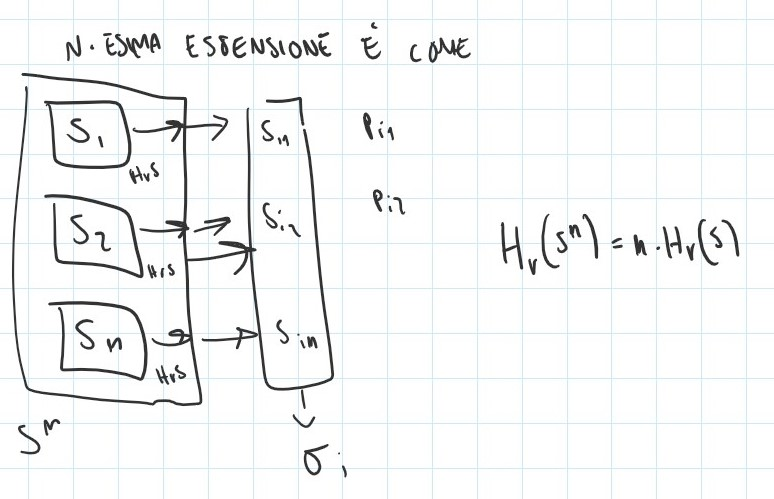
\includegraphics[width=0.72\linewidth]{immagini/img25}
\end{figure}












\newpage
\section*{Lezione 11}
\addcontentsline{toc}{section}{Lezione 11}

Riprendiamo dalla seguente disuguaglianza:

\begin{equation*}
H_r(S) \leq L_{sf} < H_r(S) + 1
\end{equation*}

\subsection*{Primo teorema di Shannon-Fano}
\addcontentsline{toc}{subsection}{Primo teorema di Shannon-Fano}

Proviamo ad applicarla all'$n$-esima estensione della sorgente:
(P.S. la $L$ è relativa a Shannon-Fano, $L_n$ è la lunghezza media delle codeword che codificano i simboli di $S^n$)

\begin{equation*}
H_r(S^n) \leq L_{n} < H_r(S^n) + 1
\end{equation*}

Da prima però sappiamo quanto vale $H_r(S^n)$:

\begin{equation*}
n \cdot H_r(S) \leq L_{n} < n \cdot H_r(S^n) + 1
\end{equation*}

\begin{equation*}
H_r(S) \leq \frac{L_{n}}{n} < H_r(S^n) + \frac{1}{n}
\end{equation*}

Quest'ultima disuguaglianza è uguale a quella iniziale con $n=1$, aumentando la $n$ l'intervallo si riduce linearmente, "si schiaccia" verso l'ottimo (teorema dei carabinieri).\\

La $L_n$ è il numero medio di bit che mi servono per rappresentare $\sigma_i$; ma diamo un'occhiata a $\sigma_i$:

\begin{equation*}
\sigma_i= (s_{i1}, s_{i2}, ... , s_{in})
\end{equation*}

Se per rappresentare $\sigma_i$ serve $L_n$, per rappresentare ogni $s_{ij}$ mi servono $\frac{L_n}{n}$ lunghezze di codeword.

Quindi le lunghezze di Shannon-Fano hanno il vantaggio di avere codeword più vicine all'ottimo al crescere di $n$, ovviamente però non posso creare estensioni troppo grandi perchè dovrei rappresentare un numero enorme di simboli.

Bello dal punto di vista teorico, ma praticamente è un disastro.
Questo risultato è il primo teorema di Shannon-Fano chiamato \textit{Noiseless coding theorem}\\
Fine codifica di sorgente

\newpage

\subsection*{Canali di comunicazione}
\addcontentsline{toc}{subsection}{Canali di comunicazione}

Un canale di comunicazione l'acqua, un filo elettrico, il tempo, ecc...
Una definizione di un modello astratto semplice da gestire ma complicato per poterlo analizzare:
\begin{figure}[h]
	\centering
	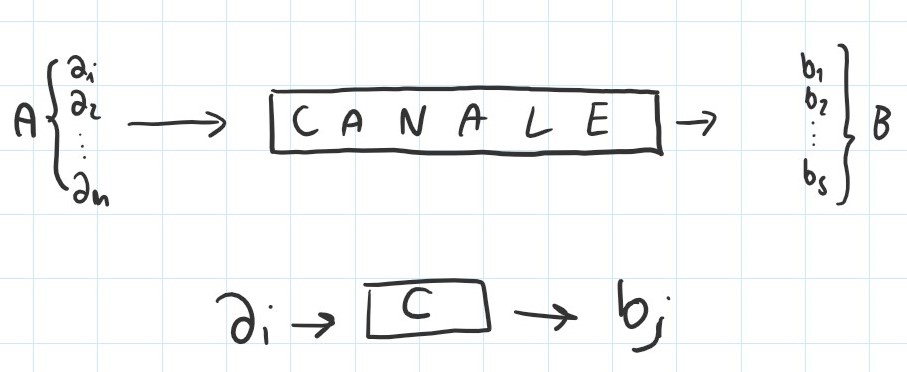
\includegraphics[width=0.8\linewidth]{immagini/img26}
\end{figure}
Esso è costituito da:
\begin{itemize}
	\item Simboli in input
	\item Simboli in output
	\item Probabilità condizionate
\end{itemize}
Ogni volta che inserisco un simbolo $a_i$ appartenente all'alfabeto $A$, il canale restituisce un simbolo $b_j$ appartenente all'alfabeto $B$.
Il rumore agisce sul simbolo $a_i$, facendo uscire un simbolo a seconda delle probabilità:
\begin{equation*}
P(b_j|a_i)
\end{equation*}
Per rappresentare tutte le probabilità condizionate uso una matrice di canale:

\begin{figure}[h]
	\centering
	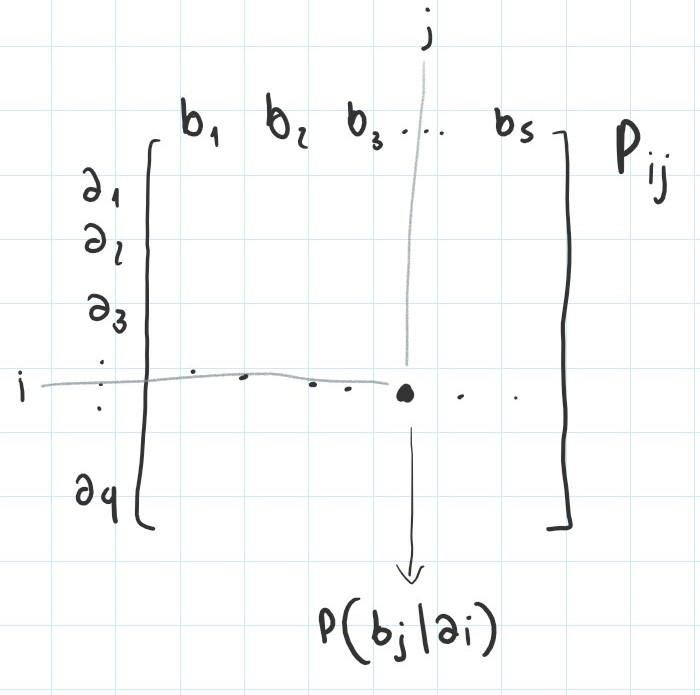
\includegraphics[width=0.57\linewidth]{immagini/img27}
\end{figure}

Quindi inserito un simbolo $a_i$ uscirà un simbolo $b$ in output basato sulle probabilità della riga $i$. Ovviamente dato un simbolo ne uscirà un altro sicuramente, quindi:
\begin{equation*}
\sum_{j=1}^sp(b_j|a_i)=\sum_{j=1}^sp_{ij} = 1
\end{equation*}
In altre parole ogni riga contiene una distribuzione discreta di probabilità, quindi la matrice è definita stocastica.

Se una riga ha tutti 0 e un 1 allora sappiamo che il simbolo su quella riga avrà sempre lo stesso simbolo in output (magari il canale è costruito in un certo modo, boh).

$p(a_i)$ è la probabilità con cui scegliamo il simbolo $a_i$ da inserire all'interno del canale. Quindi diciamo che l'utente inserisce nel canale il simbolo $a_i$ con questa probabilità.
Ci chiediamo quanto è la probabilità che esca $b_j$ (con $j=1,2,...s$).
Definiamo l'equazione di canale:
\begin{equation*}
p(b_j) =\sum_{i=1}^qp(b_j|a_i)p(a_i)
\end{equation*}
Quindi la probabilità di $b_j$ è la somma di più probabilità, in particolare ogni termine è la probabilità che esca $b_j$ dato che è stato inserito in ingresso $a_1$ oppure $a_2$ oppure $a_3$...
Il concetto viene più chiaro tramite questo grafo:
\begin{figure}[h]
	\centering
	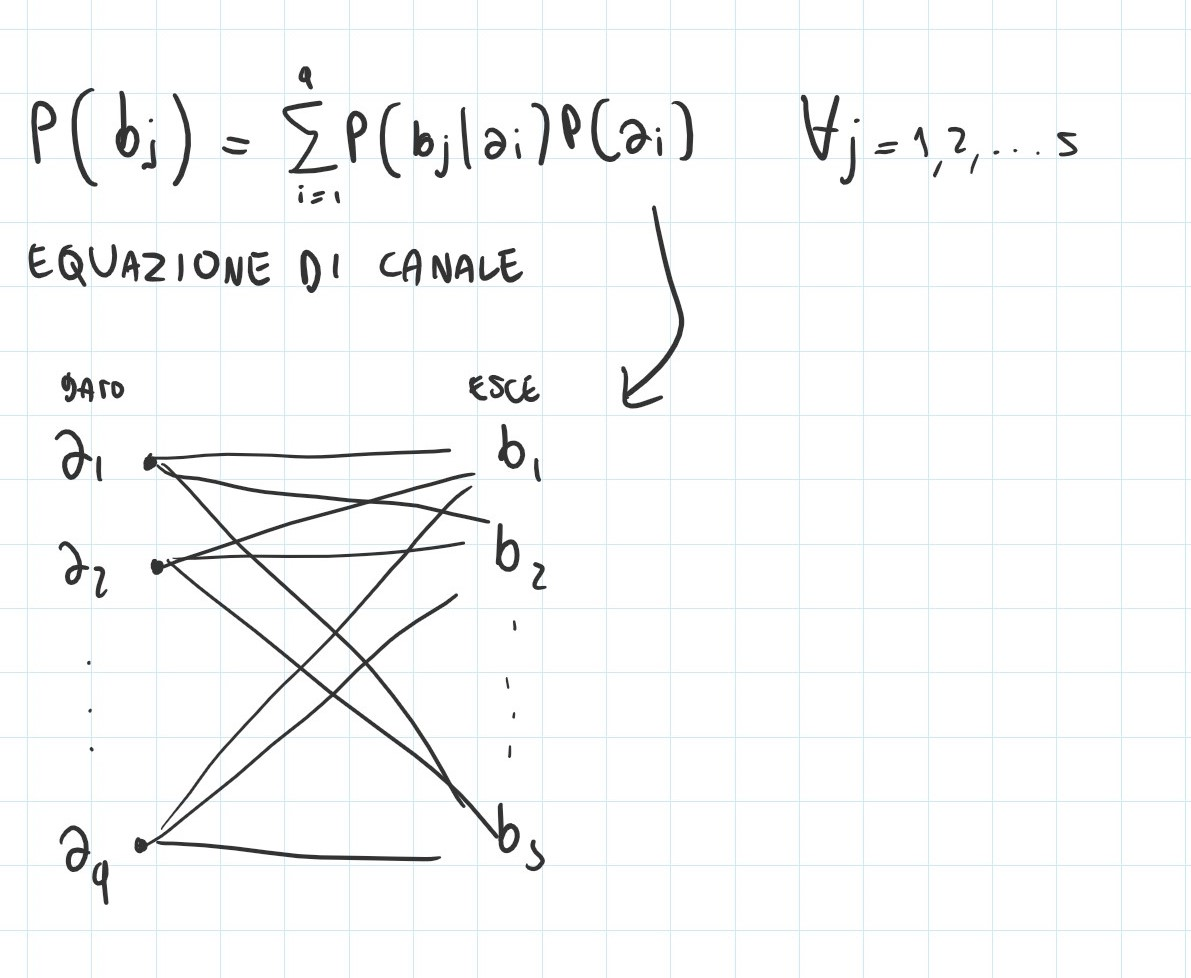
\includegraphics[width=0.85\linewidth]{immagini/img28}
\end{figure}

Vediamo ora due casi particolari (estremi, nella pratica non dovrebbero mai accadere):

\begin{itemize}
	\item Canale con assenza di rumore:\\
	Ogni volta che inserisco $a_i$ ho probabilità 1 che esca un certo $b_j$. Quindi la matrice di canale avrà tutte righe composte da 0 e 1.
	L'equazione di canale diventa:
	\begin{equation*}
	p(b_j) =\sum_{i=1}^qp(b_j|a_i)p(a_i) = 1 + 0 + ... + 0 = 1
	\end{equation*}
	\item Canale completamente rumoroso:\\
	Ogni simbolo inserito in input è completamente ignorato e l'output è totalmente casuale.
	In pratica le $b_j$ hanno una distribuzione di probabilità che dipende dal rumore e non da $a_i$.
	L'equazione di canale è:
	\begin{equation*}
	p(b_j) =\frac{1}{s} \; \; \; \; \forall j
	\end{equation*}
\end{itemize}

\subsection*{Probabilità condizionate all'indietro}
\addcontentsline{toc}{subsection}{Probabilità all'indietro}
Quando inserisco un simbolo in input $a_i$ sappiamo che la probabilità che esca $b_j$ è $p(b_j|a_i)$, ma quanto è la probabilità 'al contrario'? Ovvero, quanto è la probabilità che sia stato inviato $a_i$, visto che mi è arrivato $b_j$? Teorema di Bayes:
\begin{equation*}
p(a_i|b_j) = \frac{p(b_j|a_i)p(a_i)}{p(b_j)}
\end{equation*}
E usando l'equazione di canale:
\begin{equation*}
= \frac{p(b_j|a_i)p(a_i)}{\sum_{i=1}^qp(b_j|a_i)p(a_i)}
\end{equation*}
Consideriamo il canale più semplice (canale binario):
\begin{figure}[H]
	\centering
	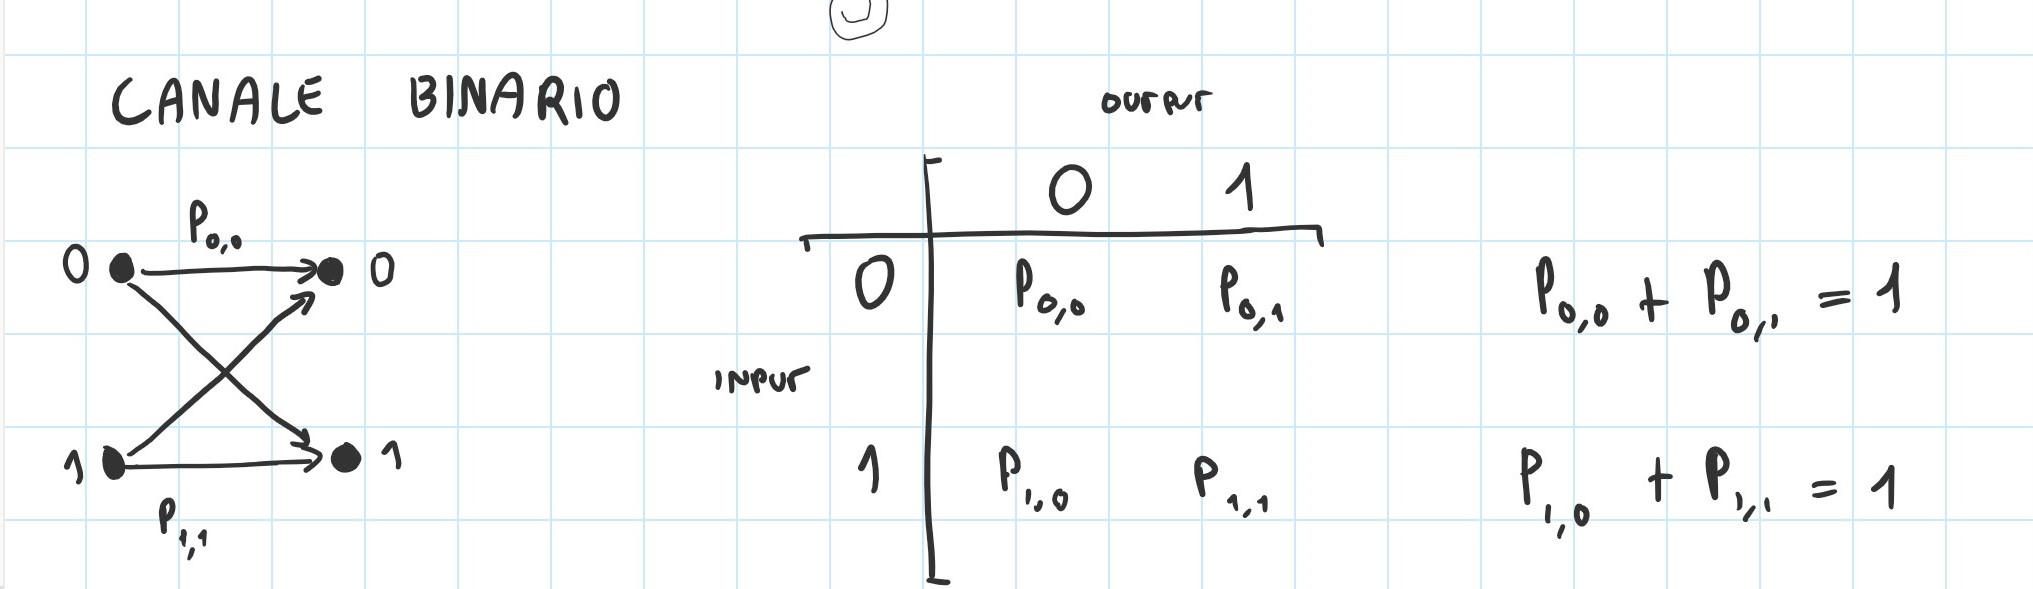
\includegraphics[width=\linewidth]{immagini/img29}
\end{figure}
La probabilità $p_{0,0} = p_{1,1}$ viene chiamata $P$, essa rappresenta la probabilità che inserito un bit dal canale esca lo stesso bit.
Chiamo $Q = 1-P$ la probabilità che la trasmissione sia errata.

La matrice di canale diventa:
\begin{equation*}
\begin{pmatrix}
P & Q\\
Q & P 
\end{pmatrix}
\end{equation*}

Questo tipo di canale è chiamato \textit{canale binario simmetrico} (CBS) in quanto la matrice che lo definisce è simmetrica.

Usando tanti canali CBS, voglio inviare un messaggio lungo $n$ bit, qual è la probabilità che il primo bit arrivi a destinazione sbagliato?\\
$Q$.\\
E che il secondo sbagli? $Q$. E così via.
I canali sono paralleli quindi gli eventi sono indipendenti (se uno sbaglia gli altri non vengono influenzati).
Questa descrizione è già stata vista: è il rumore bianco.
L'ennesima estensione della CBS ($\text{CBS}^n$) è il canale che rappresenta il rumore bianco.

Chiamo $a$ l'input del CBS e $b$ l'output. Chiamo inoltre $p$ la probabilità di scegliere $a=0$; $p(a=0)$.
Quindi $1-p$ è $p(a=1)$.
Chiamiamo $x$ la $p(b=0)$ e $1-x = p(b=1)$.
Le equazioni di canale ci dicono che:
\begin{equation*}
p(b=0) = pP + (1-p)Q
\end{equation*}
\begin{equation*}
p(b=1) = (1-p)P + pQ
\end{equation*}

Le probabilità all'indietro sono:

\begin{equation*}
p(a=0|b=0) = \frac{pP}{pP+(1-p)Q}
\end{equation*}



\newpage
\section*{Lezione 12}
\addcontentsline{toc}{section}{Lezione 12}

Riprendendo le probabilità all'indietro di prima:

\begin{equation*}
p(a=0|b=0) = \frac{pP}{pP+Q(1-p)}
\end{equation*}
\begin{equation*}
p(a=1|b=1) = \frac{P(1-p)}{pQ+P(1-p)}
\end{equation*}
\begin{equation*}
p(a=1|b=0) = \frac{Q(1-p)}{pP+Q(1-p)}
\end{equation*}
\begin{equation*}
p(a=0|b=1) = \frac{pQ}{pQ+P(1-p)}
\end{equation*}

Vediamo un esempio: $P=\frac{9}{10}$, $Q = 1-P = \frac{1}{10}$. L'utente digita con probabilità $\frac{19}{20}$ il bit 0, mentre con $\frac{1}{20}$ il bit 1.
Quindi:
\begin{equation*}
p(a=0) = \frac{19}{20}
\end{equation*}
\begin{equation*}
p(a=1) = \frac{1}{20}
\end{equation*}

Vediamo le probabilità all'indietro, quindi come il ricevente deve interpretare il messaggio:

\begin{equation*}
p(a=0\,|\,b=0) = \frac{171}{172}
\end{equation*}
\begin{equation*}
p(a=1\,|\,b=1) = \frac{9}{28}
\end{equation*}
\begin{equation*}
p(a=1\,|\,b=0) = \frac{1}{172}
\end{equation*}
\begin{equation*}
p(a=0\,|\,b=1) = \frac{19}{28}
\end{equation*}

Quindi se il ricevente ha inviato 0 confronta le probabilità che il mittente abbia inviato effettivamente 0 oppure 1:

\begin{equation*}
p(a=0\,|\,b=0) = \frac{171}{172} \; \; \; vs \; \; \; p(a=1\,|\,b=0) = \frac{1}{172}
\end{equation*}

Domina la probabilità che abbia inviato 0, quindi leggo il messaggio proprio come 0.\\
Ora mettiamo che arrivi un 1:

\begin{equation*}
p(a=0\,|\,b=1) = \frac{19}{28} \; \; \; vs \; \; \; p(a=1\,|\,b=1) = \frac{9}{28}
\end{equation*}

La probabilità che abbia inviato 0 è ancora più alta! Quindi il mittente leggerà sempre 0!\\
Come mai succede questo?\\
Il problema è che

\begin{equation*}
\begin{cases}
p(a=0\,|\,b=0) > p(a=1\,|\,b=1)\\
p(a=0\,|\,b=1) > p(a=1\,|\,b=0)\\
\end{cases}
\end{equation*}
\begin{equation*}
\begin{cases}
Pp > Q(1-p)\\
Qp > P(1-p)
\end{cases}
\end{equation*}
\begin{equation*}
\begin{cases}
Pp > (1-P)(1-p)\\
Qp > P(1-p)
\end{cases}
\end{equation*}
\begin{equation*}
\begin{cases}
\cancel{Pp} > 1 - P + \cancel{Pp} - p\\
Qp > P(1-p)
\end{cases}
\end{equation*}
\begin{equation*}
\begin{cases}
0 > 1 - P - p\\
Qp > P(1-p)
\end{cases}
\end{equation*}
\begin{equation*}
\begin{cases}
0 > 1 - P - p\\
\cancel{(1-p)}p > P\cancel{(1-p)}
\end{cases}
\end{equation*}
\begin{equation*}
\begin{cases}
p > 1 - P\\
p > P
\end{cases}
\end{equation*}
\begin{equation*}
\begin{cases}
p > Q\\
p > P
\end{cases}
\end{equation*}

Il problema qui è che l'utente ha utilizzato una distribuzione di probabilità per i simboli molto diversa dalla distribuzione uniforme.

\subsection*{Entropia congiunta}
\addcontentsline{toc}{subsection}{Entropia congiunta}

Possiamo vedere l'uscita del canale come se fosse una sorgente, quindi posso chiedermi quanto vale la quantità di informazione relativa a $b_j$ e rispetto a $a_i$, e quale rapporto c'è fra le due?\\ 
Ci sono quindi tre punti di vista: vedo solo $A$, vedo solo $B$ o le vedo entrambe e mi chiedo in che rapporto sono.

\smallskip
Partendo da $A$:

\begin{equation*}
H_r(A) = \sum_{i=1}^qp(a_i)\log_r\frac{1}{p(a_i)}
\end{equation*}

possiamo quindi scrivere anche $B$:

\begin{equation*}
H_r(B) = \sum_{j=1}^sp(b_j)\log_r\frac{1}{p(b_j)}
\end{equation*}

Dunque si può anche scrivere una entropia condizionata: un entropia sui simboli di $A$ dato che dal canale è uscito un simbolo $b_j$.

\begin{equation*}
H_r(A|b_j) = \sum_{i=1}^qp(a_i\,|\,b_j)\log_r\frac{1}{p(a_i\,|\,b_j)}
\end{equation*}

Allo stesso modo posso anche calcolare $H_r(A|B)$, che rappresenta la quantità di informazione che mediamente è uscita dal canale dato che ho visto uscire uno qualsiasi dei simboli di $B$

\begin{equation*}
H_r(A|B) = \sum_{j=1}^sp(b_j)H_r(A\,|\,b_j)
\end{equation*}

\begin{empheq}[box=\tcbhighmath]{equation*}
H_r(A|B) = \sum_{j=1}^s\sum_{i=1}^qp(a_i,b_j)\log_r\frac{1}{p(a_i\,|\,b_j)}
\end{empheq}

Questa quantità viene detta \textbf{equivocazione}.

Ora vediamo dall'altro verso, posso quindi considerare $H(B\,|\,a_i)$ quindi una quantità di informazione media su $B$ dato che so che è stato inserito un simbolo $a_i$ nel canale.

\begin{equation*}
H_r(B|a_i) = \sum_{j=1}^sp(b_j\,|\,a_i)\log_r\frac{1}{p(b_j\,|\,a_i)}
\end{equation*}

Quindi ora come prima facciamo una media pesata (questa volta sugli $a_i$):

\begin{empheq}[box=\tcbhighmath]{equation*}
H_r(B|A) = \sum_{i=1}^q\sum_{j=1}^sp(a_i,b_j)\log_r\frac{1}{p(b_j\,|\,a_i)}
\end{empheq}

L'ultima entropia da definire è l'entropia congiunta:

\begin{empheq}[box=\tcbhighmath]{equation*}
H_r(A,B) = \sum_{i=1}^q\sum_{j=1}^sp(a_i,b_j)\log_r\frac{1}{p(a_i,b_j)}
\end{empheq}

Vediamo ora diversi casi sulle probabilità:

\begin{itemize}
	\item $p(a_i,b_j)=p(a_i)p(b_j)$   $\forall i, j$\\
	Questo accade solo quando le due probabilità sono indipendenti, quindi quando inserire $a_i$ non influenza l'uscita di $b_j$, cosa che avviene solo nei canali completamente rumorosi.\\
	In questo caso l'entropia congiunta diventa:
	\begin{equation*}
	H_r(A,B) = \sum_{i=1}^q\sum_{j=1}^sp(a_i)p(b_j)\log_r\frac{1}{p(a_i)p(b_j)}
	\end{equation*}
	\begin{equation*}
	H_r(A,B) = \sum_{i=1}^q\sum_{j=1}^sp(a_i)p(b_j)[\log_r\frac{1}{p(a_i)} +  \log_r\frac{1}{p(b_j)}]
	\end{equation*}
	\begin{equation*}
	H_r(A,B) = \sum_{j=1}^sp(b_j)\sum_{i=1}^qp(a_i)\log_r\frac{1}{p(a_i)} +
	\sum_{i=1}^qp(a_i)\sum_{j=1}^sp(b_j)\log_r\frac{1}{p(b_j)}
	\end{equation*}
	\begin{equation*}
	H_r(A,B) = 1 \cdot H_r(A) +
	1 \cdot H_r(B)
	\end{equation*}
	Quindi nel caso di canale completamente rumoroso ho che l'entropia congiunta $H_r(A,B)$ che è la quantità di informazione media che ottengo guardando contemporaneamente la sorgente $A$ e la sorgente $B$ (terzo punto di vista di prima).
	
    \item $p(a_i, b_j)=p(a_i)p(b_j\,|\,a_i)$   $\forall i, j$\\
    Questo è il caso 'normale', quindi c'è rumore bianco:
    \begin{equation*}
	H_r(A,B) = \sum_{i=1}^q\sum_{j=1}^sp(a_i,b_j)\log_r\frac{1}{p(a_i)}+\sum_{i=1}^q\sum_{j=1}^sp(a_i,b_j)\log_r\frac{1}{p(b_j|a_i)}
    \end{equation*}
    Ora sfruttiamo una proprietà statistica per cui:
    \begin{equation*}
    \sum_{j=1}^sp(a_i, b_j) = p(a_i)
    \end{equation*}
    Questa proprietà si chiama \textit{marginale} di $a_i$.
    Quindi proseguo in questo modo:
    \begin{center}
    	... conti ...
	    \end{center}
	\begin{empheq}[box=\tcbhighmath]{equation*}
	H_r(A,B) = H_r(A) + H_r(B|A)
	\end{empheq}
	Quindi la somma della quantità di informazione effettivamente inserita nel canale più l'equivocazione. Quest'ultima agisce come rumore.
	Se non ci fosse rumore l'entropia $H_r(A,B) = H_r(A)$.
\end{itemize}
C'è una simmetria in tutte queste formule fra $A$ e $B$, scambiandoli i risultati non cambiano, infatti possiamo esprimere l'entropia congiunta anche in questo modo:
\begin{equation*}
H_r(A,B) = H_r(B) + H_r(A|B)
\end{equation*}

\subsection*{Mutua informazione}
\addcontentsline{toc}{subsection}{Mutua informazione}
Quanto è la quantità di informazione che viene trasmessa all'interno del canale? Quella che viene trasmessa dall'inizio alla fine del canale. In altre parole la quantità di informazione massima che un canale può trasportare.
Questa caratteristica non dipende da come l'utente usa il canale ma è una caratteristica intrinseca dello stesso. Essa però non potrà mai superare la capacità del canale.
\begin{equation*}
I(a_i;b_j) = \log_r\frac{1}{p(a_i)} - \log_r\frac{1}{p(a_i\,|\,b_j)} = \log_r\frac{p(a_i\,|\,b_j)}{p(a_i)}
\end{equation*}

\begin{equation*}
= \log_r\frac{p(a_i\,|\,b_j)\cdotp(b_j))}{p(a_i)\cdot p(b_j)} =  \log_r\frac{p(a_i,b_j)}{p(a_i)\cdot p(b_j)} 
\end{equation*}

Inoltre 

\begin{equation*}
= I(a_i;b_j) \leq I(a_i) = \log_r\frac{1}{p(a_i)}
\end{equation*}

Questo perchè

\begin{equation*}
= I(a_i;b_j) = log_r\frac{p(a_i\,|\,b_j)}{p(a_i)} = log_rp(a_i\,|\,b_j) + I(a_i)
\end{equation*}

$p(a_i\,|\,b_j) \leq 1 $ e il logaritmo di un valore $\leq 1$ è negativo, quindi sto riducendo il valore.

Se le distribuzioni di probabilità di $a_i$ e $b_j$ sono indipendenti, allora $I(a_i;b_j) = 0$ visto che nelle equazioni di prima questo termine:

\begin{equation*}
\log_r\frac{p(a_i\,|\,b_j)}{p(a_i)\cdot p(b_j)}
\end{equation*}

si annulla






 
\newpage
\section*{Lezione 13}
\addcontentsline{toc}{section}{Lezione 13}

Abbiamo detto che la capacità è difficile da calcolare perchè dipende dalla distribuzione dei simboli di ingresso e di uscita (che poi dipendono da quelli in entrata).\\
Quindi abbiamo detto magari ci sono dei canali in cui questi conti sono più semplici: i canali uniformi.\\
La matrice di questi canali contiene righe che sono l'una la permutazione dell'altra, ad esempio il canale binario simmetrico:
\begin{equation*}
\begin{pmatrix}
P & Q\\
Q & P
\end{pmatrix}
\end{equation*}
Perchè il canale uniforme ci semplifica il conto? Perchè la mutua informazione del sistema può essere scritta come:
\begin{equation*}
I(A;B)= H_r(B)-H_r(B\,|\,A) = H_r(B) - \sum_{A}\sum_{B}P(a,b)\log_r\frac{1}{P(B\,|\,A)}
\end{equation*}
\begin{equation*}
= H_r(B) - \sum_{A}p(a)\underbrace{\sum_{B}P(b\,|\,a)\log_r\frac{1}{P(b\,|\,a)}}_{\text{*}}
\end{equation*}

Andiamo a considerare la sommatoria (*), noi stiamo considerando la matrice di canale (dove ogni cella è $p(b\,|\,a)$), quindi il primo termine della somma, ci stiamo muovendo su una riga fissata (quella $a_i$).\\
Dato che il canale è uniforme, il risultato su ogni riga è uguale in quanto ogni riga è una permutazione dell'altra (li sommo solo in ordine differente).
Diciamo che:
\begin{equation*}
w = \sum_{B}P(b\,|\,a)\log_r\frac{1}{P(b\,|\,a)} = H_r(B\,|\,a)
\end{equation*}
Quindi $w$ ha un valore fissato che è uguale per tutte le righe e non dipende da $a$, quindi ottengo:
\begin{equation*}
= H_r(B) - w \sum_{A}p(a)
\end{equation*}
\begin{equation*}
= H_r(B) - w = I(A;B)
\end{equation*}

e questo è più è semplice da calcolare rispetto a $H_r(B)-H_r(B\,|\,A)$.

Facciamo un esempio con un canale binario simmetrico. 
\begin{equation*}
\begin{pmatrix}
P & Q\\
Q & P
\end{pmatrix}
\end{equation*}
La capacità è uguale a $H_2(B) - w$ dove
\begin{equation*}
w = P\log_2\frac1P+Qlog_2\frac1Q = 
\end{equation*}
\begin{equation*}
= P\log_2\frac1P+(1-P)log_2\frac{1}{1-P} = H_2(P)
\end{equation*}
\begin{equation*}
= Q\log_2\frac{1}{1-Q}+Qlog_2\frac{1}{Q} = H_2(Q)
\end{equation*}

Entrambi i valori sono uguali all'entropia di una bernoulliana.
\begin{equation*}
I(A;B)=H_2(B) - H_2(P)=H_2(B) - H_2(Q)
\end{equation*}
Ricordiamo che
\begin{equation*}
C=max(H_2(B)-H_2(P))
\end{equation*}
Siccome $H_2(P)$ è una costante, occupiamoci sono di massimizzare $H_2(B)$. Abbiamo già visto che questa funzione ha valore massimo 1 quanto $x=\frac12$. Quanto è però il valore di $p$ tale per cui $H_2(B)$ ha come $x=\frac12$?
\begin{equation*}
x = \frac12 = pP + (1-p)Q
\end{equation*}
\'E quindi la probabilità che venga mandato un 0 e arrivi uno 0 più la probabilità che venga mandato 1 e arrivi 0.
\begin{equation*}
= pP + (1-P)-p(1-P)
\end{equation*}
\begin{equation*}
 = 1-P-p + 2pP
\end{equation*}
\begin{equation*}
= 1 - P - p(1 - 2P)
\end{equation*}
\begin{equation*}
\downarrow
\end{equation*}
\begin{equation*}
p(1-2P) = \frac12 - P
\end{equation*}
\begin{equation*}
p\cancel{(1-2P)} = \frac{\cancel{1-2P}}{2}
\end{equation*}
Posso semplificare in quanto $(1-2P) = 0$ solo in caso di $P=\frac12$ e quindi di canale totalmente rumoroso.
\begin{equation*}
p = \frac{1}{2}
\end{equation*}

Quindi esiste un valore di $p$ che mi consente di ottenere $x=\frac12$ per cui $H_2(B)$ ottiene valore massimo, quindi ho che:

\begin{equation*}
C = 1 - H_2(P)
\end{equation*}
\begin{equation*}
C = 1 - H_2(Q)
\end{equation*}

\newpage
\subsection*{Secondo teorema di Shannon}
\addcontentsline{toc}{subsection}{Secondo teorema di Shannon}
Questo teorema mette insieme tutto quello che abbiamo detto, cioè raccoglie cosa vuol dire fare trasmissioni all'interno di un canale rumoroso applicando codici a correzione d'errore e cercando di sfruttare il canale al miglior modo possibile, quindi cercando di avvicinarsi al più possibile alla capacità di canale.

\begin{theorem}
	Dato un canale rumoroso è sempre possibile avvicinarsi in maniera arbitraria alla capacità del canale mantenendo contemporaneamente arbitrariamente bassa la probabilità d'errore.
\end{theorem}

Quindi abbiamo un canale rumoroso, e questo canale ha una certa capacità (il massimo al variare delle $p(a)$ della mutua informazione del sistema).\\
Questo teorema dice che è possibile avvicinarsi arbitrariamente al valore della capacità (tipo asintoto). Avvicinarsi vuol dire trovare delle codeword, o una codifica, per cui ci si avvicina.
\medskip
Avvicinandomi alla capacità del canale inserisco sempre più informazione, e mandandone sempre di più ovviamente sbaglia sempre di più, e sbagliando di più si aumenta la probabilità che il ricevente sbagli a correggere una codeword (due errori e si corregge male).

La \textbf{5} si riferisce alla probabilità che il ricevente \textit{corregga male} una codeword.

\subsection*{Dimostrazione - Secondo teorema di Shannon}
\addcontentsline{toc}{subsection}{Dimostrazione - Secondo teorema di Shannon}
\subsubsection*{Preliminari matematici:}
\addcontentsline{toc}{subsubsection}{Preliminari matematici}
\begin{itemize}
	\item \begin{equation*}
	\sum_{k=0}^{\lambda n}\binom{n}{k} \leq 2^{nH(\lambda)} \; \; \; \;\; \text{per } 0 < \lambda < 1 \; \; \; \; \text{e } \lambda n \text{ intero}
	\end{equation*}
	
	Dove $H(\lambda)$ è l'entropia di una sorgente bernoulliana con due simboli di probabilità $\lambda$ e $1-\lambda$.
	
	\item Legge debole dei grandi numeri:\\
	Supponiamo di avere $n$ variabili casuali indipendenti fra loro ($x_1, x_2, ..., x_n$) tutte con la stessa distribuzione di probabilità caratterizzata da media $\mu$ e varianza $\sigma^2$.\\
	Allora abbiamo che per ogni $\epsilon > 0$ e per ogni $\delta> 0$ esiste un interno $n_0$ tale che per ogni $n\geq n_0$ vale che:
	\begin{equation*}
	P(|\frac1n\sum_{i=1}^nX_i-\mu| \leq \epsilon) \geq 1 - \delta
	\end{equation*}
	oppure in maniera equivalente:
	\begin{equation*}
	P(|\frac1n\sum_{i=1}^nX_i-\mu| > \epsilon) < \delta
	\end{equation*}
	
	Notiamo che $\frac1n\sum_{i=1}^nX_i$ è la media campionaria dei miei $n$ esperimenti, mentre $\mu$ è la media teorica.
	Quindi sottraendoli in valore assoluto mi chiedo quanto sono distanti (teoria e pratica).\\
	La probabilità che questa distanza superi un valore $\epsilon$ piccolo a piacere può essere resa piccola a piacere $\delta$.\\
	Nel nostro caso ogni esperimento sarà l'invio di un bit all'interno di un canale binario simmetrico.\\
	Metto $n$ copie del canale binario simmetrico ($n$-esima estensione) indipendenti fra loro, quindi la probabilità teorica di ottenere errori è $Qn$ ($\mu$).
	\smallskip
	
	In pratica inviare pacchetti tramite $n$-esima estensione CDS ($\text{CDS}^n$) equivale a trasmettere pacchetti di $n$ bit col modello del rumore bianco.\\
	
	Assumeremo che $Q < \frac12$ (se fosse maggiore metto una porta \texttt{not}, se uguale ho canale completamente rumoroso).
	
	\item Regola di decisione: essa è la regola/funzione che il ricevente applica per cercare di capire quale secondo lui è il simbolo che è stato spedito. Esempio (probabilita all'indietro $P(a_i\,|\,b_j)$):

	\[
	\kbordermatrix{
		& b_1 & b_2 & b_3 \\
		a_1 & 0.6 & 0.5 & 0.4 \\
		a_2 & 0.4 & 0.5 & 0.6
	}
	\]
	
	Assumiamo che la distribuzione delle $a_i$ sia uniforme, quindi $p(a_1) = p(a_2) = \frac12$.\\
	
	La funzione di decisione di massima verosimiglianza $d:B\rightarrow A$ è definita in queto modo:
	\begin{itemize}
		\item $d(b_1) = a_1$
		\item $d(b_3) = a_2$
		\item $d(b_2) = a_1 \lor d(b_2) = a_2$		
	\end{itemize} 

	Da notare come questa regola non abbia un unico risultato ($b_2$).
	La regola di verosimiglianza funzione in questo modo:
	\begin{equation*}
	d(b_j) = a^* \;\;\; \text{t.c.} \;\;\; P(a^*\,|\,b_j) \geq P(a_i\,|\,b_j) \; \; \forall i
	\end{equation*}
	Applicando Bayes sto dicendo che:
	\begin{equation*}
	\frac{p(b_j\,|\,a^*)p(a^*)}{\cancel{p(b_j)}} \geq \frac{p(b_j\,|\,a_i)p(a_i)}{\cancel{p(b_j)}}
	\end{equation*}
	Abbiamo detto che, non sapendo a priorio la distribuzione dei simboli di ingresso, assumo che sia uniforme; quindi:
	\begin{equation*}
	p(b_j\,|\,a^*)\cancel{\frac1q} \geq p(b_j\,|\,a_i)\cancel{\frac1q}
	\end{equation*}
	\begin{equation*}
	p(b_j\,|\, a^*) \geq p(b_j\,|\,a_i)
	\end{equation*}
	
	\item Capacità di un $\text{CBS}^n$: $n \times C$, dove $C=n(1-H_2(P)) = n(1-H_2(Q))$
\end{itemize}

\subsubsection*{Dimostrazione:}
\addcontentsline{toc}{subsubsection}{Dimostrazione}
N.B. $a_i$ e $b_j$ sono pacchetti di $n$ bit.\\
I messaggi validi fra tutte le $n$-ple di bit di A è $|A|=M\leq 2^n$. Diciamo inoltre che sono equiprobabili, quindi $p(a_i) = \frac1M$, quindi la quantità di informazione $I(a_i) = \log_2\frac{1}{\frac1M} = \log_2M$.\\
Il nostro obiettivo è quello di avvicinarci alla capacità del canale, che è:
\begin{equation*}
\text{Capacità CBS}^n = n \times C
\end{equation*}
Scelgo un $\epsilon_1 > 0$ piccolo a piacere, e chiedo che la quantità di informazione si avvicini per meno di una quantità proporzionale a $\epsilon_1$ alla capacità, quindi:
\begin{equation*}
I(a_i)=nC - \epsilon_1
\end{equation*}
Anche se in realtà questa $\epsilon_1$ dovrebbe funzionare (è più \textit{fair}) in relazione al numero di estensioni $n$, quindi:
\begin{equation*}
I(a_i)=n(C - \epsilon_1)
\end{equation*}
Da questa relazione possiamo ricavare $M$:
\begin{equation*}
M = 2^{n(C-\epsilon_1)} = \frac{2^{nC}}{2^{n\epsilon_1}}
\end{equation*}

Ora mettiamoci nei panni del ricevente: una volta ricevuto $b_j$ si costruisce una iper-sfera centrata in $b_j$ e avrà un raggio lungo $nQ$ in quanto mi aspetto $nQ$ errori.
Ora osservo che $b_j$ non sia un codice valido, quindi devo scegliere il messaggio più vicino a $b_j$ all'interno della sfera.

\begin{figure}[h]
	\centering
	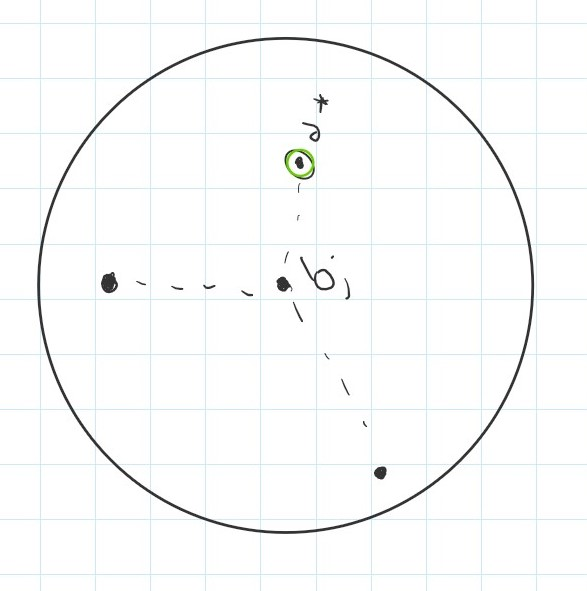
\includegraphics[width=0.45\linewidth]{immagini/img30}
\end{figure}

Quindi, data la distanza D fra $b_j$ e $a^*$ la probabilità
\begin{equation*}
p(b_j\,|\,a^*) = Q^D(1-Q)^{n-D}
\end{equation*}
per $Q < \frac12$ è decrescente al crescere di $D$, quindi la probabilità che ottenga questo $b_j$ da $a_i$ è tanto più bassa quanto sono lontani $a_i$ e $b_j$, quindi la distanza non è solo topologica.\\
In altre parole scelgo una $a^*$ che mi minimizza questa quantità: $Q^D(1-Q)^{n-D}$.\\
Il problema è che può essere complicato trovare quello più vicino e che può esserci una $a^*$ che ha la stessa distanza fra due $b_j$ (le regole di massima verosimiglianza non sono uniche).






\end{document}
